\documentclass[hidelinks,a4paper, 11pt]{article}

\usepackage[utf8]{inputenc}
\usepackage{amsmath,amsthm,verbatim,amssymb,amsfonts}
\usepackage{mathtools}
\usepackage{graphicx}
\usepackage{titlesec}
\usepackage{marvosym}
\usepackage[toc,titletoc,title]{appendix}
\usepackage{hyperref}
\usepackage{framed}
\usepackage{enumitem}
\usepackage{parskip}
\usepackage[a4paper]{geometry}
\usepackage{adjustbox} % Used to constrain images to a maximum size 
\usepackage{physics}
\usepackage{hyperref}
\usepackage{array}

\usepackage{xcolor}
\hypersetup{
	colorlinks,
	linkcolor={red!50!black},
	citecolor={red!50!black},
	urlcolor={red!50!black}
}



% change spacing around theorems
\makeatletter
\def\thm@space@setup{%
	\thm@preskip=7mm
	\thm@postskip=\thm@preskip % or whatever, if you don't want them to be equal
}
\makeatother

% bold title for optional title in theorems
\makeatletter
\def\th@plain{%
	\thm@notefont{}% same as heading font
	\itshape % body font
}
\def\th@definition{%
	\thm@notefont{}% same as heading font
	\normalfont % body font
}
\makeatother

\theoremstyle{plain}
\newtheorem{theorem}{Theorem}
\newtheorem{lemma}[theorem]{Lemma}
\newtheorem{collorary}[theorem]{Collorary}
\newtheorem{behauptung}{Behauptung}
\newtheorem{corollary}{Corollary}
\newtheorem{proposition}{Proposition}
\newtheorem*{surfacecor}{Corollary 1}
\newtheorem*{frage}{Frage}


\newtheoremstyle{break}% name
	{}%         Space above, empty = `usual value'
	{}%         Space below
	{}% Body font
	{}%         Indent amount (empty = no indent, \parindent = para indent)
	{\bfseries}% Thm head font
	{.}%        Punctuation after thm head
	{\newline}% Space after thm head: \newline = linebreak
	{}%         Thm head spec

\theoremstyle{break}


\theoremstyle{plain}
\newtheorem{definition}[theorem]{Definition}

\theoremstyle{definition}
\newtheorem*{example}{Example}
\newtheorem*{bem}{Bemerkungen} 
\newtheorem*{remark}{Remark}

\newcommand{\rom}[1]{\uppercase\expandafter{\romannumeral #1\relax}}
\newcommand{\R}{\mathbb R}
\newcommand{\vbreak}{\vspace{8mm}}

% Notizbox
\setlength{\marginparsep}{6mm}
\setlength{\marginparwidth}{18mm}



\begin{document}

\title{3236 L 125: Mathematical Physics I\\ \large{Dynamical Systems and Classical Mechanics} }
\author{Lecture by Yuri B. Suris \\ Technical University Berlin \\ Winter term 2018}
\date{ Notes by Viet Duc Nguyen}

\maketitle
\tableofcontents

\setcounter{section}{-1}
\section{About the notes}
These are \emph{personal} lecture notes for the course \emph{Mathematical Physics I: Dynamical Systems and Classical Mechanics}, which is a undergraduate and graduate course of the Berlin Mathematical School held at the Technical University Berlin. The lecture was held by Professor Yuri B. Suris in the winter term 2018. As pointed out, these lecture notes are \emph{personal} notes written by me for the course; thus it may contain mistakes!

Letters in bold typefaces usually refer to vectors in $\mathbb R^n$, e.g. $\mathbf x = (x_1,...,x_n)^T$.

\textit{Literature recommendations by Professor Suris: V. Arnold, Mathematical Methods of Classical Mechanics; V. Arnold, Ordinary differential equations; A. Knauf, Mathematische Physik: Klassische Mechanik}

\section{Introduction: Basic Principles of Dynamical Systems}

\marginpar{\textbf{Week 01}\\ Tue, 16.10}
States of a dynamical system are denoted by the \emph{phase space} $X$. The phase space $X$ is a vector space in $\mathbb R^n$ or a manifold. The evolution of states is described either by continuous time or discrete time. The entire future and past of a dynamical system is completely determined by one state $\mathbf x_0$ at any fixed moment of time $t_0 = 0$. If the world were purely described by dynamical systems, we would live in a completely deterministic world!

The one parameter family of maps $\Phi^t: X \to X, \mathbf x_0 \mapsto \mathbf x(t,\mathbf x_0)$ describes the evolution of any state $\mathbf x_0$ for time $t$. $\Phi^t$ is called a phase flow. It can be continuous $(\Phi^t)_{t \in \mathbb R}$ or discrete $(\Phi^t)_{t \in \mathbb Z}$.

We collect some properties of phase flows:
\begin{itemize}
	\item $\mathbf x(0, \mathbf x_0) = \mathbf x_0$ for all $\mathbf x_0 \in X$ if and only if $\Phi^{0} = \mathrm{id}_X$
	\item $\mathbf x(t+s, \mathbf x_0) = \mathbf x(t, \mathbf x(s, \mathbf x_0))$ for all $\mathbf x_0 \in X$ and for all $t,s \in \mathbb R$
	\item $\Phi^t \circ \Phi^{-t} = \Phi^{t-t} = \Phi^0 = \mathrm{id}_X \iff \Phi^{-t} = (\Phi^t)^{-1}$ for all $t \in\mathbb R$
\end{itemize}

A $1$-parameter family of maps $(\Phi^t)_{t \in G}$ ($G$ is an abelian group written additively, e.g. $G = \mathbb R$ or $G = \mathbb Z$) with properties $\Phi^0 = \mathrm{id}_X$ and $\Phi^{t+s} = \Phi^t \circ \Phi^s = \Phi^{s+t}$ is called an action of $G$ on $X$ of a dynamical system with phase space $X$ and time $G$.  

\section[Ordinary differential equations]{Existence and uniqueness of solutions of  ordinary differential equations}

\marginpar{\textbf{Week 01}\\Thu, 18.10}

Consider the system of \emph{first-order ordinary\footnote{First-order means that only a derivative of rank one occurs. Ordinary means that one derives only after one variable, i.e. there are no partial derivatives.}} differential equations:
\begin{gather*}
	\mathbf{\dot x} = f(t, \mathbf x), \quad \mathbf x = \begin{pmatrix}
		x_1 \\ \vdots \\ x_n
	\end{pmatrix}, \quad \text{and}\quad  f= \begin{pmatrix}
		f_1 \\ \vdots \\ f_n
	\end{pmatrix}.
\end{gather*}

We can rewrite the system of ODEs (ordinary differential equations) as
\[
	\begin{cases} 
	\dot x_1 = f_1(t,x_1,...,x_n) \\
	\quad \quad \vdots \\
	\dot x_n = f_n(t,x_1,...,x_n).
	\end{cases}.
\]

The question is: When is a function $x: I \to U\footnote{$I \subset \mathbb R$ and $U \subset \mathbb R^n$}$ a solution of the ODE? And especially: \underline{When is a solution unique?}


\begin{definition}[Lipschitz continuous]
	Let $f$ be a function. $f$ is locally Lipschitz continuous with respect to $x$ if and only if $\forall (t_0,x_0) \in \Omega, \exists \text{ neighborhood } \Omega_0 \subset \Omega \text{ of } (t_0,x_0) \text{ and } L > 0 \text{ such that: }$
	\[
		||f(t,x_1) - f(t,x_2)|| \leq L ||x_1-x_2||, \quad \forall (t,x_1), (t,x_2) \in \Omega_0.
	\]
\end{definition}


\begin{definition}[Solution of differential equations]
	Let $I \subset \R$ be an \underline{interval} and $f: \Omega \to \mathbb R^n$. A function $x: I \to \R^n$ is called a solution of an ODE $\dot x = f(t,x)$ if
	\begin{itemize}
		\item $x$ is differentiable on $I$,
		\item $(t,x(t)) \in \Omega$ for all $t \in I$,
		\item $\dot x(t) = f(t,x(t))$ for all $t \in I$.
	\end{itemize}
\end{definition}


\subsection{Existence of solutions}

\begin{theorem}[Local existence after Picard-Lindelöf]
	Let $f: \Omega \to \R^n$ be locally Lipschitz continuous. Consider $(t_0,x_0) \in \Omega$. Then, there exists one $\delta >0$ such that the initial value problem
	\begin{align}\label{chap2:IVP}
		\begin{cases}
			\dot x = f(t,x) \\x(t_0) = x_0
		\end{cases} 
	\end{align}
	has a solution on $I = (t_0-\delta, t_0 + \delta)$.
\end{theorem}

\begin{proof}
	We only provide a sketch of proof.
	\begin{enumerate}
		\item Reformulate the IVP \eqref{chap2:IVP} as integral equation
		\[
			x(t) = x_0 + \int^t_{t_0} f(s,x(s)) ds.
		\]
		Note that the integral exists since $f$ is continuous.
		
		\item Choose a compact neighborhood $$K=\underbrace{[t_0 - a, t_0 + a]}_{\coloneqq I \subset \mathbb R} \times \underbrace{\{ x : ||x-x_0|| \leq b\}}_{\coloneqq U \subset \R^{n}} \subset \Omega.$$
		Let $M \coloneqq \max_{(t,x) \in K} || f(t,x) ||$ ($M$ exists because $K$ is compact) and consider the function space $\mathcal M$ with:
		\begin{gather*}
			\mathcal M = \mathcal M_{a,b} = \{ \gamma \in C^0(I, \R^n) \, \vert \, \forall t \in I: ||\gamma(t) - x_0|| \leq b \}.
		\end{gather*}
		
		$\mathcal M$ is a complete, metric space (Banach space) of continuous functions with a metric given by: $$d(\gamma_1, \gamma_2) = \max_{t \in I}{||\gamma_1(t)-\gamma_2(t)||}.$$
		
		Define an operator $P: \mathcal M_{a,b} \to \mathcal M_{a,b}$ that takes a function $y$ and maps it to another function $P_y$:
		\[
			(P_y)(t) = x_0 + \int^t_{t_0}f(s,y(s)) ds.
		\]
		
		Is $P_y \in \mathcal M_{a,b}$? Indeed:
		\[
			|| P_y(t) - x_0 || = ||x_0 +  \int^t_{t_0}f(s,y(s)) ds -x_0 || = || \int^t_{t_0}f(s,y(s)) ds || \overset{(*)}{\leq} Ma \leq b.
		\]
		We get the inequality $(*)$ by the mean value theorem. If $Ma > b$, we can adjust $a$ such that $a \leq \frac{b}{M}$.
		
		\item We construct the Picard-iterations:
		\[
			y^{(0)}(t) \coloneqq x_0, \quad y^{(n+1)}(t) \coloneqq P_{y^{(n)}}(t), \quad t \in I.
		\]
		We claim that $P_{y^{(n)}} \to y^{*}$ for $n \to \infty$ with $P_{y^*} = y^*$. In other words: $y^*$ is a fixed point of $P$ and we found a solution for the ODE \eqref{chap2:IVP}.
		
		We will only show that the iterations converge but we do not show that it actually converges to the fixed point of $P$. We could prove the converge to the fixed point by showing that $P$ is a contraction but instead, observe that:
		\begin{align*}
			y^{(n)}(t) &= y^{(0)}(t) + (y^{(n)}(t) - y^{(n-1)}(t)) + (y^{(n-1)}(t) - y^{(n-2)}(t))+... \\
			&= y^{(0)}(t) + \sum^n_{k=1}y^{(k)}(t) - y^{(k-1)}(t)
		\end{align*}
		So convergence of $\big(y^{(n)}(t)\big)^{\infty}_{n=0}$ is equivalent to convergence of the series $\sum^{\infty}_{k=1}y^{(k)}(t) -y^{(k-1)}(t)$. Let $L$ be the Lipschitz constant of $f$. We will show that
		\[
			\Vert y^{(n+1)}(t) - y^{(n)}(t) \Vert \leq \frac{M}{L} \left( \frac{(L |t-t_0|)^{n+1}}{(n+1)!} \right).
		\]
		This is done by induction. Induction base for $n=0$:
		\[
			\Vert y^{(1)}(t) - y^{(0)}(t) \Vert = \Vert \int^t_{t_0} f(s,x_0) ds \Vert \leq M |t-t_0|.
		\]
		$n \leadsto n+1$:
		\begin{align*}
			\Vert y^{(n+1)}(t) - y^{(n)}(t) \Vert &= \Vert \int^t_{t_0} \left(f\big(s,y^{(n)}(s)\big) - f\big(s,y^{(n-1)}(s)\big)\right) ds \Vert && \text{Lipschitz continuous} \\
			&\leq L \int^t_{t_0}  \Vert y^{(n)}(s) - y^{(n-1)}(s) \Vert ds&& \text{induction basis} \\
			& \leq L \int^t_{t_0} \frac{M}{L}\left(\frac{(L |s-t_0|)^n}{n!}\right) ds && \text{integrate} \\
			&= \frac{M}{L}\frac{(L|t-t_0|)^{n+1}}{(n+1)!}
		\end{align*}
		We showed the convergence of the Picard iterations.
	\end{enumerate}
\end{proof}

\subsection{Uniqueness of solutions}

\marginpar{\textbf{Week 02}\\Tue, 23.10}


Remember: $\dot x = f(t,x), \quad (t,x) \in I \times U = \Omega \subset \mathbb R^{n+1}, I \subset \mathbb R, U \subset \mathbb R^n,$ where $I$ is the time space and $U$ is the phase space.

\begin{theorem}[Uniqueness theorem]
	Let $f: \Omega \to \mathbb R^n$ be locally Lipschitz continuous with respect to $x$. If $x^{(1)}: I \to \mathbb R, x^{(2)}: I \to \mathbb R$ are two solutions of $\dot x = f(t,x)$ with $x^{(1)}(t_0) = x^{(2)}(t_0)$ for some $t_0 \in I$, then $$x^{(1)}(t) = x^{(2)}(t), \quad \forall t \in I.$$
\end{theorem}

This follows from the  \emph{Lemma of Gronwall}. So we will show this lemma first, and then use it to prove the theorem of uniqueness.

\begin{theorem}[Lemma of Gronwall]
	Let $a,b,w: [t_0, t_0 +c] \to \mathbb R_{\geq 0}$ be three non-negative functions satisfying 
	\[
		w(t) \leq a(t) + \int^t_{t_0} b(s)w(s) ds, \quad \forall t \in [t_0, t_0 + c].
	\]
	Then there holds:
	\[
		w(t) \leq a(t) + \int^t_{t_0} a(s)b(s) e^{\int^t_sb(\tau) d\tau}ds, \quad \forall t \in [t_0, t_0 + c].
	\]
\end{theorem}

\begin{proof}
	Let $y(t) \coloneqq \int^t_{t_0} b(s)w(s) ds$. If we prove that the following holds
	\[
		y(t) \leq \int^t_{t_0}a(s)b(s)e^{\int^t_s b(\tau)d\tau}ds,
	\]
	we get the claim since $w(t) \leq a +y(t)$. We know that $w(t) \leq a(t) + y(t)$, so it follows $w(t)-y(t) \leq a(t)$. Now, lets multiply this with $b(t)$ and since $b$ is non-negative, we get:
	\begin{align*}
		\underbrace{w(t)b(t)}_{=y'(t)} - y(t)b(t) \leq a(t)b(t).
	\end{align*}
	Multiply this with $e^{-\int^t_{t_0}b(s)ds}$
	\[
		\underbrace{\Big(y'(t) - y(t)b(t)\Big)e^{-\int^t_{t_0}b(s)ds}}_{=\frac{d}{dt}\left(y(t)e^{-\int^t_{t_0}b(s)ds}\right) } \leq a(t)b(t) e^{-\int^t_{t_0}b(s)ds}.
	\]
	So we get
	\[
		\frac{d}{dt}\left(y(t)e^{-\int^t_{t_0}b(s)ds}\right)  \leq  a(t)b(t) e^{-\int^t_{t_0}b(s)ds}.
	\]
	We integrate both sides with $\int^t_{t_0}$ and since $y(t_0) = 0$ we get:
	\[
		y(t)e^{-\int^t_{t_0}b(s)ds} \leq \int^t_{t_0}a(s)b(s) e^{-\int_{t_0}^s b(\tau) d\tau}ds
	\]
	In the end, we multiply by $e^{\int_{t_0}^t b(s) ds}$ and we get our final result
	\[
		y(t) \leq  \int^t_{t_0}a(s)b(s) \underbrace{e^{-\int^{s}_{t_0} b(\tau)d\tau}}_{=e^{\int_{s}^{t_0} b(\tau) d\tau}} e^{\int_{t_0}^t b(s) ds}ds = \int^t_{t_0}a(s)b(s) e^{\int^t_s b(\tau)d\tau}ds.
	\]
\end{proof}

\begin{remark}
This lemma is useful to estimate $w$ with known functions $a$ and $b$. There are three particular cases: 
\begin{enumerate}
	\item Let $b(s) = b = \text{constant}$. So it holds:
	 \[
	w(t) \leq a(t) + b \int^t_{t_0}w(s) ds \implies w(t) \leq a(t) + b \int^t_{t_0}a(s)e^{b(t-s)}ds.
	\]
	
	\item Let $a(s) = a = \text{constant}$ and $b(s) = b = \text{constant}$. One can show that:
	\[
		w(t) \leq a+b \int^t_{t_0}w(s)ds \implies w(t) \leq ae^{b(t-t_0)}
	\]
	
	\item Let $a=0$ and let $b = b(s) = \text{constant}$. \begin{framed}
	\begin{align}\label{chap2:gronwallcase3}
		w(t) \leq b\int^t_{t_0}w(s)ds \implies w = 0.
	\end{align}\end{framed}
\end{enumerate}
\end{remark}

Next, we will prove the uniqueness lemma which is not that difficult anymore.
\begin{proof}[Proof of the uniqueness theorem]
	Let $J \subset I$ be a closed interval with $t_0 \in J$. Then the solution curves $x^{(1)}, x^{(2)}: J \to \mathbb R$ are compact. Set $w(t) \coloneqq \Vert x^{(1)}(t)-x^{(2)}(t) \Vert$. Remember that $\dot x = f(s,x)$. Then for $t \in J$ we have:
	\begin{align*}
		w(t) &= \Vert \int^t_{t_0} f(s, x^{(1)}(s)) - f(s,x^{(2)}(s)) ds \Vert \\
		&\leq L \int^t_{t_0}\Vert x^{(1)}(s) - x^{(2)}(s) \Vert ds,
	\end{align*}
	where $L$ is the maximal local Lipschitz constant over $J$. Note that $L$ exists since $J$ is compact and $f$ is continuous (it is even local Lipschitz continuous).
	\[
		w(t) \leq L \int^t_{t_0}\Vert x^{(1)}(s) - x^{(2)}(s) \Vert ds = L \int^t_{t_0}w(s)ds \overset{\eqref{chap2:gronwallcase3}}{\implies} w(t) = 0, \quad \forall t \in J.
	\]
\end{proof}

\begin{remark}
	If $f(t,x)$ is not locally Lipschitz continuous, then uniqueness may not hold and as a rule of thumb, there will be no uniqueness of solutions. Murphy's Law in action. The IVP 
	\begin{align}\label{chap2:nouniqueness}
		\dot x = \sqrt[3]{x^2}, \quad x(0) = 0
	\end{align}
	has an infinite solutions. For instance, there are solutions with $x(t) = 0$ or for $b > 0$:
	\begin{align*}
		x_b(t) = \begin{cases}
		0, \quad & \text{for $t < b$} \\
		\frac{1}{27}(t-b)^3, \quad & \text{for $t \geq b$}.
		\end{cases}
	\end{align*}
\end{remark}

\subsection[Continuation of Solutions]{Continuation of solutions}
\begin{definition}
	We say that a solution $x: (t_0,t_1) \to \mathbb R^n$ can be \emph{continued} to the right if there exists a solution $\tilde x : (t_0,t_2) \to \mathbb R^n$ with $t_2 > t_1$ such that:
	\[
		\tilde x(t) = x(t), \quad \forall t \in (t_0,t_1).
	\]
	We say that $x$ is a \emph{maximal} solution if it cannot be continued neither to the right nor to the left.
\end{definition}

\begin{theorem}
	Let $x: (t_0,t_1) \to \mathbb R^n$ be a solution for $\dot x = f(t,x)$ and $f: \Omega \to \mathbb R^n$. A solution $x$ can be continued to the right if and only if there exists the limit $x_1 \coloneqq \lim_{t\nearrow t_1}x(t)$ and $(t_1,x_1) \in \Omega$.
\end{theorem}
\begin{proof}
	Assume the limit exists $x_1 = \lim_{t\nearrow t_1}x(t)$. We can apply the uniqueness and existence theorem to show that the $x$ can be continued to the right. Consider the IVP with $x(t_1) = x_1$. There exists a solution on $(t_1-\delta, t_1 + \delta)$ for the IVP which we call $y$. Define $\tilde x$ as follows:
	\[
		\tilde x(t) \coloneqq \begin{cases}
			x(t), \quad & \text{for $t \in (t_0,t_1)$} \\
			y(t), \quad & \text{for $t \in (t_1,t_1 + \delta)$}
		\end{cases}.
	\]
	We expanded the solution on $(t_0,t_1 + \delta)$. This function $\tilde x(t)$ is also continuous due to $$\lim_{t\nearrow t_1} \tilde x(t) = \lim_{t\nearrow t_1}x(t) = x_1 = y(t_1) = \tilde x(t_1).$$
	
	The other direction is easy(?). I don't know...
\end{proof}

\begin{theorem}[Theorem about maximal solutions]\label{theorem:maximalsolutions}
Let $f: \Omega \to \mathbb R^n$ be locally Lipschitz continuous with respect to $x$ and let $x: (t_-,t_+) \to \mathbb R^n$ be a maximal solution of $\dot x = f(t,x)$. Then:
\begin{itemize}
	\item either $t_+ = \infty$,
	\item or $t_+ < \infty$ and for each \underline{compact} set $K \subset \Omega$ there exists $t' < t_+$ such that
	\[
		\forall t \in (t', t_+): \big(t,x(t)\big) \notin K.
	\]
	In other words, $x(t)$ leaves any compact subset $K \subset \Omega$, which usually means that $x(t)$ becomes infinite in finite time.
\end{itemize}
\end{theorem}

\begin{remark}
	The only reason for a solution to have finite time is the blow-up within finite time. Consider the ODE
	\begin{align} \label{chap2:blowup}
		\dot x = x^2.
	\end{align}
	It has solutions $x(t) = \frac{1}{c-t} \to \infty$ for $t \nearrow c$.
\end{remark}

\begin{theorem}[No blow-up for linearly growing $f$]
	If $\Vert f(t,x) \Vert \leq \alpha(t)\Vert x \Vert + \beta(t)$ for all $(t,x) \in I \times \mathbb R^n$, then the maximal solutions are defined on the whole intervall $I$ (usually $I = \mathbb R$).
\end{theorem}

\begin{remark}
	If $\Vert f(t,x) \Vert$ grows as $\Vert x \Vert^p$ with $p > 1$, one should expect blow-up. For $p < 1$, the uniqueness of solutions is not granted, see \eqref{chap2:nouniqueness}. For $p > 1$, it usually blows up, see \eqref{chap2:blowup}.\\
	
	\adjustimage{max size={0.5\linewidth}{0.5\paperheight}}{chap2_abs.png}
	\adjustimage{max size={0.5\linewidth}{0.5\paperheight}}{chap2_x2.png}
\end{remark}

\subsection{Dependence of solutions on initial data and on parameters}
Consider the IVP
\[
	\begin{cases}
		\dot x = f(t,x) \\x(t_0) = x_0
	\end{cases}
\]
with solution $x(t,t_0,x_0)$. We use additional parameters $(t_0,x_0)$ to highlight the dependency of the solution $x(t)$ on the initial value. How does a solution $x(t,t_0,x_0)$ depend on $x_0$?

\begin{theorem} \label{chap2:dependenceofsolution.simple} 
	Let $f: \Omega \to \mathbb R^n$ be continuously differentiable with respect to $x$. Then the solution $x(t,t_0,x_0)$ is continuously differentiable with respect to $x_0$. The Jacobi matrix
	\[
		y \coloneqq \frac{\partial x(t,t_0,x_0)}{\partial x_0} \in \mathrm{Mat_{n \times n}}
	\]
	solves \emph{Poincare's variational equation}:
	\begin{align} \label{poincarevariational}
		\begin{cases}
			\dot y = A(t)y  \\
			y(t_0) = I_{n \times n}
		\end{cases} \text{with} \quad  
		A(t) &\coloneqq \frac{\partial f(t,x)}{\partial x} \Big \vert_{x=x(t,t_0,x_0)}  \\
		&= \frac{\partial f}{\partial x}\big(t,x(t,t_0,x_0) \big). \nonumber
	\end{align}
\end{theorem}

\begin{theorem}
	Let $f$ depend on some parameters $\lambda \in \mathbb R^p$, so that 
	\[
		f: \mathbb R \times \mathbb R^n \times \mathbb R^p \supset \Omega \to \mathbb R^n
	\]
	is $\mathcal C^1$ with respect to $x$ and $\lambda$. Consider the IVP
	\[
		\begin{cases}
			\dot x = f(t,x, \lambda), \\
			x(t_0) = x_0
		\end{cases}
	\]
	with solution $x(t, t_0,x_0, \lambda)$. Then the function $x(t,t_0,x_0,\lambda)$ is continuously differentiable with respect to $\lambda$ and the Jacobi matrix 
	\[
		y \coloneqq \frac{\partial x (t,t_0,x_0,\lambda)}{\partial \lambda} \in \mathrm{Mat}_{n \times p}
	\]
	solves the following IVP:
	\begin{align*}
		\begin{cases}
			\dot y = Aty + B(t) \\
			y(t_0) = 0_{n \times p}
		\end{cases}\text{with} \quad 
		A &\coloneqq \frac{\partial f}{\partial x} (t,x(t), \lambda) \\
		B &\coloneqq \frac{\partial f}{\partial \lambda}\big(t,x(t), \lambda \big).
	\end{align*}
\end{theorem}

\section{Dynamical systems}
\marginpar{\textbf{Week 02}\\Thu, 25.10}

\subsection{Autonomous differential equations}
Loosely spoken: autonomous differential equations $\equiv$ dynamical systems with continuous time. Let $f: \mathbb R^n \supset U \to \mathbb R^n$ be a vector field and locally Lipschitz continuous. Consider the ODE with
\[
	\dot x = f(x).
\]
This means, the law of motion does not depend on time. The system is completely deterministic. In other words, the instantaneous velocity $\dot x$ only depends on the position $x$ and not on the moment of time $t$ at which the system arrives at $x$.

\begin{remark}
	We observe: if $x: I \to U$ is a solution of $\dot x = f(x)$, then $y(t) \coloneqq x(t- \tau)$ is a solution, as well.
\end{remark}

\begin{proof}
	$\dot y(t) = \dot x(t- \tau) = f(x(t - \tau)) = f(y(t)).$
\end{proof}

\begin{remark}
	Try the proof for a non-autonomous ODE $\dot x = f(t,x)$ with solution $y(t) \coloneqq x(t- \tau)$.
	\[
		\dot y(t) = \dot x(t-\tau) = f(t-\tau, x(t- \tau)) = f(t-\tau, y(t)) \neq f(t, y(t)) \quad21 \text{\Lightning}
	\]
\end{remark}

\begin{definition}[Group]
	A group $(G,*)$ is a set $G$ together with $* : G \times G \to G$ such that 
	\begin{itemize}
		\item $\forall g,h \in G: g * h \in G$ (closure),
		\item $\forall g,h,k \in G: (g * h)*k = g * (h * k)$ (associativity),
		\item $\forall g \in G, \exists! e \in G: g * e = e * g = g$ (neutral element),
		\item $\forall g \in G, \exists h \in G: g * h = h* g = e$ (inverse element).
	\end{itemize}
\end{definition}

\begin{definition}[Left group action]
	Let $M$ be a set and $G$ be a group. The left action of $G$ on $M$ is the map $\Phi_g: G \times M \to M, (g,x) \mapsto \Phi_g(x)$ such that
	\begin{enumerate}
		\item $\forall g,h \in G, x\in M: \Phi_{g+h}(x) = \Phi_g(\Phi_h(x)) = (\Phi_g \circ \Phi_h)(x)$,
		\item $\exists! e \in G,\forall x \in M: \Phi_e(x) = x$.
	\end{enumerate}
	If these two axioms are satisfied, then $\Phi_g$ is a bijection from $M$ to $M$ for fixed $g$.
\end{definition}



\subsection{Realisation of dynamical systems}

We now know that every initial value problem 
\[
\begin{cases}
	\dot x = \mathbf f(t,x) \\ x(t_0) = x_0
\end{cases}
	\quad \text{where } \mathbf f \in \mathcal C^k(I \times M\footnote{$I \subset \mathbb R, M \subset \mathbb R^n$}, \mathbb R^n), k \geq 1
\]
has a local solution $\varphi(t,t_0,x_0)$ that is of class $\mathcal C^k$ with respect to $(t,t_0,x_0)$. Moreover, the solution can be extended in time until either reaches the homology of $M$ or blows up at infinity.

So, what is a dynamical system? It is a mathematical formalisation of a \underline{deterministic} process. A dynamical system consists of 
\begin{itemize}
	\item a complete metric space $M$, which is called \emph{phase space}. It constains all possible states of a region. We assume that $\dim M < \infty$.
	
	\item a time variable $\underbrace{t \in \mathbb R, \mathbb R_+}_{\text{continuous time}}$  or $\underbrace{t \in \mathbb Z, \mathbb Z_+}_{\text{discrete time}}$.
	
	\item and a law of evolution in time (time evolution operator).
\end{itemize}

\begin{definition}[Dynamical system]
	Let $M \subset \mathbb R^n$ be a phase space. Let $G$ be a number set with a group structure ($G \subset \mathbb R$) and $g \in G$ denotes the time variable. A \emph{dynamical system} is a triple $\{ \Phi_y, G,M \}$ defined in terms of the $G$-action:
	\begin{align*}
	\Phi_G : G \times M, (g,x) \mapsto \Phi_g(x) \tag{\textit{time evolution operator}}
	\end{align*}
\end{definition}
If we consider $G = \mathbb R$ and $G * G \to G, g *h \coloneqq g + h$, we have an abelian group. For every left group action holds: $\Phi_{g+h}(x) = \Phi_g(\Phi_h(x)) = \Phi_h(\Phi_g(x)) = \Phi_{h+g}(x)$.\\

\textbf{How do we define dynamical systems in terms of initial value problems?}

Consider a continuous dynamical system $\{ \Phi_t, \mathbb R, M \}, M \subset \mathbb R^n$.  The time evolution operator $\Phi_t$ is the \emph{global flow} of an autonomous IVP
	\begin{align}\label{chap3:simpleIVP}
		\dot x = f(x), x(0) = x_0 \in M.
	\end{align}
	That means, that $\Phi_t$ solves the IVP above. Let $\varphi$ be the unique local solution of \eqref{chap3:simpleIVP}. So $\Phi_t$ is defined as
	\[
		\Phi_t: \mathbb R \times M \to M, (t,x) \mapsto \Phi_t(x) \coloneqq \varphi(t,x).
	\]
The following properties hold
\begin{enumerate}
	\item $\Phi_{t+s}(x) = (\Phi_t \circ \Phi_s)(x)$ for every $t,s \in \mathbb R$ and $x \in M$
	\begin{center}
			\adjustimage{max size={0.6\linewidth}{0.6\paperheight}}{Chap3_Figure1.png}
	\end{center}

	
	\item $\Phi_0(x) = x$ for every $x \in M$
	
	\item $\Phi_t \circ \Phi_{-t} = \mathrm{id_M}$.
\end{enumerate}

\begin{definition}[Orbit]
An \emph{orbit} starting at  $x_0 \in M$ is the ordered subset of $M$ defined by $$\mathcal O(x_0) = \{ x \in M : x = \Phi_g(x_0), \forall g \in G \}.$$ It is a parametrised curve in the phase space $M$.
\end{definition}
\begin{center}
	\adjustimage{max size={0.4\linewidth}{0.4\paperheight}}{Chap3_Figure2.png}
\end{center}

\begin{remark}
	If $y_0 = \Phi_g(x_0)$ for some $g \in G$, then the sets $\mathcal O(x_0)$ and $\mathcal O(y_0)$ are equal. Different orbits are disjoint.
\end{remark}

\begin{definition}[Fixed point, cycle, phase portrait, invariant set, invariant functions]\ { }
	\label{definition:fixedpoint}
	\begin{enumerate}
		\item A point $\tilde x \in M$ is a \emph{fixed point} if $\tilde x = \Phi_G(\tilde x)$ for every $g \in G$.
		
		\item A \emph{cycle} is an orbit $\mathcal O(x_0)$ such that each point $x \in \mathcal O(x_0)$ satisfies
		\[
			\Phi_{g+T}(x) = \Phi_g(x), \forall g \in G \text{ with some fixed } T > 0.
		\]
		The minimal $T$ is called the period.
		
		\item The \emph{phase portrait}  is a partitioning of $M$ into orbits (collection of orbits).
		
		\item An \emph{invariant set} is a subset $S \subset M$ such that $\Phi_g(S) \subset S$ for every $g \in G$.
		
		\item An \emph{invariant function} is a function $F: M \to \mathbb R$ such that $F(\Phi_g(x)) = F(x)$ for all $g \in G, x \in M$. This means that the $F$ cannot distinguish between points in an orbit.
	\end{enumerate}
\end{definition}

\begin{remark}
	The IVP in \eqref{chap3:simpleIVP} is autonomous (independent of time). This means that the IVP has a time-translational symmetry. \underline{We can always set $t_0 = 0$.} If $\varphi(t,x_0)$ with $t \in I_{x_0}$ is a solution for the IVP with initial value $t(0) = x_0$, so is $\psi(t,x_0) = \varphi(t+s,x_0)$ with $t+s \in I_{x_0}$. We get
	\[
		\dot \psi(t,x_0) = \dot \varphi(t+s,x_0) = f(\varphi(t+s,x_0)) = f(\psi(t,x_0)).
	\]
\end{remark}

\begin{example}
	Not every flow is global. Consider $W: \bigcup_{x_0 \in M} I_{x_0} \times \{ x_ 0 \} \subset \mathbb R \times M$ where $I_{x_0}$ is the maximal intervall on which a solution $\varphi$ exists for the IVP with initial value $x(0) = x_0$. Look at the scalar differential equation:
	\[
	\begin{cases}
	\dot x = x^3 \\ x(0) = x_0, x_0 \in M
	\end{cases}
	\]
	The flow is defined as 
	\begin{gather*}
	W = \{ (t,x_0) : 2tx_0^2 < 1 \}, \\
	I_{x_0} = (- \infty, \frac{1}{2x_0^2}) ,\\
	\Phi_t: W \to \mathbb R, (t,x_0) \mapsto \varphi(t,x_0) = \frac{x_0}{\sqrt{1-2x_0^2t}}.
	\end{gather*}
\end{example}


\textbf{Graphical interpretations}

A solution $t \mapsto \varphi(t,x_0)$ defines for each $x_0 \in M$ two curves:
\begin{enumerate}
	\item A solution curve (integral curve, trajectory curve): 
	\[
		\gamma(x_0) = \{ (t,x) : x=\Phi_t(x_0), \forall t \in I_{x_0} \} \subset I_{x_0} \times M.
	\]
	
	\item An orbit or the projection of $\gamma(x_0)$ on $M$ is
	\[
		\mathcal O(x_0) = \{ x: x = \Phi_t(x_0), \forall t \in I_{x_0} \} \subset M.
	\]
	An orbit cannot intersect itself. If two orbits have a common point, they coincide.
\end{enumerate}

\begin{remark}
The zeros of $f$ of \eqref{chap3:simpleIVP} define the fixed points. If $f(\tilde x ) = 0$, then $\Phi_t(\tilde x) = \tilde x$ for every $t \in I_{x_0}$.
\end{remark}

\marginpar{\textbf{Week 03}\\Tue, 30.10}

\textbf{From autonomous ordinary differential equations to dynamical systems:} Consider the IVP
$
	\begin{cases}
		\dot x = f(x) \\
		x(0) = x_0
	\end{cases}
$
with solution $x(t,0,x_0)$. Define the flow as:
\[
	\Phi^t_{x_0} \coloneqq x(t,0,x_0) \quad \text{and} \quad \Phi^t: X \to X, x_0 \mapsto \Phi^t_{x_0}
\]
It holds:
\begin{enumerate}[label=(\arabic*)]
	\item $\Phi^0 = \mathrm{id_X}$
	\item $\Phi^t \circ \Phi^s = \Phi^s \circ \Phi^t = \Phi^{t+s}$
\end{enumerate}

\begin{proof}
	We only prove the second statement. Consider the Taylor expansion at $t_0=0$:
	\begin{align*}
		x(t,0,x_0) = x(0) + \sum^\infty_{i=1}\frac{x^{(i)}(0,0,x_0)}{i!} t 
		= x_0 + \sum^\infty_{i=0}\frac{f^{(i)}(0)}{i!} t 
	\end{align*}
	It holds that
	\begin{align*}
		x(s,0,x(t,0,x_0)) &= x(t,0,x_0)+ \sum^\infty_{i=0}\frac{f^{(i)}(0)}{i!} s \\
		&= x_0 + \sum^\infty_{i=0}\frac{f^{(i)}(0)}{i!} t  + \sum^\infty_{i=0}\frac{f^{(i)}(0)}{i!} s  \\
		&= x_0 + \sum^\infty_{i=0}\frac{f^{(i)}(0)}{i!} (t+s)\\
		&= x(t+s,0,x_0). 
	\end{align*}
\end{proof}

\textbf{From a dynamical system to an autonomuous ODE:} Let $(\Phi_t, \mathbb R, M), M \subset \mathbb R^n$ be a continuous dynamical system. We obtain the corresponding IVP by:
\begin{align*}
	f(x) = \frac{d}{dt}\Phi^t(x) \Big \vert_{t=0}.
\end{align*}

\subsection{Diffeomorphism, Lie derivative and integral of motion}

We will show that maps $\Phi^t$ are local diffeomorphisms. Before, we need the following lemma.
\begin{lemma}[Liouville's formula]\label{formula:liouville}
	Let $I \subset \mathbb R$ be an intervall and $A: I \to \mathbb R^{n \times n}$ continuous. Let $Y: I \to \mathbb R^{n \times n}$ be a \emph{general} solution for the ODE
	\begin{align}\label{chap3:detproofreq}
		\dot y = A(t)y.
	\end{align}
	Then for all $t,t_0 \in I$, it holds:
	\begin{align}\label{chap3:liouville}
		\det Y(t) = \det Y(t_0) e^{\int^t_{t_0} \mathrm{tr} A(z) dz}.
	\end{align}
\end{lemma}

\begin{proof}
	We will compute $\frac{d}{dt}\det Y(t)$. Since $\det Y(t)$ is multilinear with respect to all entries $Y_{ij}$ of the matrix $Y$, it holds for a fixed $i \in \{1,...,n\}$
	\begin{align}\label{chap3:proofdet}
		\det Y = \sum^n_{j=1} Y_{ij} \underbrace{(-1)^{i+j} \det \tilde Y_{ij}}_{\coloneqq u_{ij}} = \sum^n_{j=1} Y_{ij}u_{ij}.
	\end{align}
	The $u_{ij}$ are also called \emph{cofactors}. So we have with chain rule and product rule applied on $\det$:
	\begin{align*}
		\frac{d}{dt}\det Y = \sum^n_{i,j = 1} \frac{\partial \det Y}{\partial Y_{ij}} \dot Y_{ij} \overset{\eqref{chap3:proofdet}}{=} \sum^n_{i,j = 1}u_{ij} \dot Y_{ij} &\overset{\eqref{chap3:detproofreq}}{=} \sum^n_{i,j = 1}u_{ij} \left( \sum^n_{k=1} A_{ik}(t)Y_{kj} \right) \\
		&= \sum^n_{i,k = 1}A_{ik}(t)\underbrace{\sum^n_{j=1} Y_{kj}u_{ij}}_{(*)} \\
		&= \mathrm{tr}A(t) \cdot \det Y.
	\end{align*}
	$(*)$ means that if $i=k$, this is $\det Y$ by \eqref{chap3:proofdet}.
	
	If $i \neq k$, $(*)$ is zero since $(*) = \det(\text{matrix } Y \text{ with row } i \text{ replaced by row }k)$.
	\\	
	
	Transforming the last equation yields
	\[
		\frac{\frac{d}{dt}\det Y(t)}{\det Y(t)} = \frac{d}{dt}\ln(\det Y(t)) = \mathrm{tr}A(t).
	\]
	Now we integrate with arbitrary $t_0 \in I$ and apply the exponential function
	\[
		\ln(\det Y(t)) - \ln(\det Y(t_0)) = \int^t_{t_0}\mathrm{tr}A(z)dz \implies \det Y(t) = \det Y(t_0)e^{\int^t_{t_0}\mathrm{tr}A(z)dz }.
	\]
\end{proof}

\begin{collorary}\label{chap3:colloraryliouville}
	\begin{align}\label{chap3:colloraryliouvilleeq}
		\exists t_0 \in I: \det Y(t_0) \neq 0 \implies \forall t \in I: \det Y(t) \neq 0
	\end{align}
\end{collorary}
\begin{proof}
	Since $e^c \neq 0$ for all $c \in \mathbb R$ and we can chose $t_0$ such that $\det Y(t_0) \neq 0$, it holds that for all $\det Y(t) \neq 0$ after \eqref{chap3:liouville}.
\end{proof}

\begin{theorem}
	Maps $\Phi^t$ are local diffeomorphisms.
\end{theorem}
\begin{proof}
It is clear that $\Phi^t$ is differentiable and continuous. By theorem about inverse functions, we just need to show that $\frac{\partial}{\partial x_0}\Phi^t$ exists and is invertible. As said, the derivative exists and we show that the determinant of the invert of the derivative is non-zero (and thus invertible):
\[
	\det \left( \frac{\partial }{\partial x_0}\Phi^t \right)  \neq 0.
\]
We know from theorem \eqref{chap2:dependenceofsolution.simple} that $Y(t) \coloneqq \frac{\partial}{\partial x_0}\Phi^t = \frac{\partial x(t,0,x_0)}{\partial x_0}$ satisfies a linear differential equation $$\begin{cases}\dot  Y = A(t) \cdot Y\\ Y(0) = I\end{cases}$$ with $A(t) = \frac{\partial f(x(t,0,x_0))}{\partial x}$. Now we can use the result of collorary \eqref{chap3:colloraryliouville}:
\[
	\det Y(0) = \det I = 1 \neq 0 \overset{\eqref{chap3:colloraryliouvilleeq}}{\implies} \forall |t| < \delta(x_0): \det Y(t) = \det \left( \frac{\partial }{\partial x_0}\Phi^t \right) \neq 0.
\]
\end{proof}

\begin{remark}
	If $\delta$ can be chosen one and the same for all $x_0 \in X$, then $\Phi^t$ is defined for all $t \in \mathbb R$ and for all $x_0 \in X$. Then $\Phi^t$ is a \emph{global} diffeomorphism.
\end{remark}

It is useful to know how some function $F: X \to \mathbb R$ evolves along solutions $\Phi^t(x)$. Thus, we consider $F(\Phi^t(x))$. This is studied by considering
\[
	\frac{d}{dt} F(\Phi^t(x)) = dF(\Phi^t(x)) \cdot \frac{d}{dt}\Phi^t = dF(\Phi^t(x)) \cdot f(\Phi^t(x)).
\]
We can omit the arguments:
\[
	\frac{dF}{dt} = \dot F = dF \cdot f = \sum^n_{k=1} \left(\frac{\partial F}{\partial x_k} f_k \right).
\]
\begin{definition}[Lie derivative] \label{chap3:liederivativedefinition}
	The \emph{Lie derivative} of the function $F$ along the vector field $f(x)$ is defined as:
	\[
	\mathcal L_fF(x) \coloneqq \frac{d}{dt} F(\Phi^t(x)) \Bigg \vert_{t=0} = \sum^n_{k=1}f_k(x)\frac{\partial F}{\partial x_k}(x).
	\]
	One often writes $\mathcal L_f$ as an operator acting on functions $F: X \to \mathbb R$
	\[
	\mathcal L_f = \sum^n_{k=1} f_k(x) \frac{\partial}{\partial x_k}.
	\]
\end{definition}

\begin{definition}[Conserved quantity, first integral of motion]\label{chap3:conservedquantitydef}
	A function $F: X \to \mathbb R$ is a conserved quantity or first integral of motion or simply an integral of the ODE $\dot x = f(x)$ if 
	\[
		\forall t: F(\Phi^t(x))  = F(x).
	\]
\end{definition}

\begin{theorem}
	$F: X \to \mathbb R$ is a conserved quantity iff $\mathcal L_fF = 0$.
\end{theorem}

\begin{remark}
	Given a function $F$ and a vector field $f$, it is straightforward to check, whether $F$ is a conserved quantity for $\dot x = f(x)$.
	
	The problem of finding an integral of motion $F$ for a given vector field $f$ is usually very complicated, for it consists of    solving a partial differential equation 
	\[
		\sum f_k \frac{\partial F}{\partial x_k} = 0.
	\] 
\end{remark}

\begin{example}
	Let $U: \mathbb R^n \to \mathbb R$ be the potential energy. Consider the ODE:
	\[
		\ddot X  = - \frac{\partial U(x)}{\partial x}.
	\]
	Written as first order ODE:
	\[
		\begin{cases}
			\dot x = u \\
			\dot u = - \frac{\partial U(x)}{\partial x}.
		\end{cases}
	\]
	We claim that $\epsilon(x,u) \coloneqq \frac{1}{2}\langle u,u \rangle + U(x)$ is an integral of motion. The vector field is
	\[
		f(x,u) = \begin{pmatrix}
			u \\ - \frac{\partial U(x)}{\partial x}.
		\end{pmatrix} \text{ with } u \in \mathbb R^n, - \frac{\partial U(x)}{\partial x} \in \mathbb R^n.
	\]
	Check that this is indeed an integral of motion:
	\begin{align*}
		\mathcal L_f \epsilon = \sum^n_{k=1} \frac{\partial \epsilon}{\partial x_k}u_k + \sum^n_{k=1} \frac{\partial \epsilon}{\partial x_k}\left(-\frac{\partial U(x)}{\partial x_k}\right) =  \sum^n_{k=1} \frac{\partial U}{\partial x_k}u_k + \sum^n_{k=1} u_k\left(-\frac{\partial U(x)}{\partial x_k}\right) = 0.
	\end{align*}
	Note, that $(\frac{1}{2}\langle u,u \rangle)_k = \frac{1}{2}u_k^2$ and therefore $(\frac{d}{2du}\langle u,u \rangle)_k = u_k$. Since we have $\mathcal L_f \epsilon = 0$, $\epsilon$ is indeed an integral of motion.
\end{example}

\begin{example}[Lotka-Volterra system]
	Let $x$ denote the number of hares, and $y$ denote the number of foxes. Consider the ODE
	\[
		\begin{cases}
		\dot x = ax-by \\
		\dot y = -cy +dy
		\end{cases}
	\]
	with $a,b,c,d > 0$. This possess an integral of motion
	\[
		F(x,y) = dx-by-c \ln(x) - a\ln(y).
	\]
	Check:
	\begin{align*}
		\mathcal L_fF = (d - \frac{c}{x})\underbrace{(ax - by)}_{=f_1} + (-b-\frac{a}{y})\underbrace{(-cy+dy)}_{=f_2} = 0.
	\end{align*}
\end{example}

\begin{remark}
	If $F$ is an integral of motion for an ODE $\dot x = f(x)$, then the level sets of $F$ are the orbits of the flows $\Phi^t$. For instance, let $Q \coloneqq \{ x : F(x) = y \}$ be the level set of $y$. Then $Q \supset \mathcal O(y)$.
\end{remark}

\begin{remark}
	If the level sets are closed curves, then all solutions $\Phi^t(x_0) = x(t,0,x_0)$ and hence all orbits are periodic.
\end{remark}

\begin{definition}[Conserved quantity for discrete systems]
	A function $F: X \to \mathbb R$ is called a conserved quantity or an integral of motion of a discrete dynamical system $(\Phi^n)_{n \in \mathbb Z}$ iff 
	\[
		\forall n \in \mathbb Z, \forall x: F(\Phi^n(x)) = F(x)
	\]
\end{definition}
\begin{remark}
	We have no Lie derivatives to check this! But it is sufficient to validate for $n=1$, i.e.
	\[
		\forall x: F(\Phi(x)) = F(x).
	\]
\end{remark}

\subsection{Commutator of vector fields}


\marginpar{\textbf{Week 03}\\Thu, 01.11}


\begin{definition}[Lie algebra]
	A Lie algebra is a vector space $\mathcal H$ supplied with a blinear operation $$[\cdot,\cdot]: \mathcal H \times \mathcal H \to \mathcal H$$ with the properties:
	\begin{itemize}
		\item for all $f,g,h \in H$ and for all $a,b \in \mathbb R$: $[af+bg,h] = a[f,h] + b[g,h]$,
		\item for all $f,g,h \in H$ and for all $a,b \in \mathbb R$: $[f,ag+bh] = a[f,g] + b[f,h]$,
		\item $[f,g] = [g,f]$ (skew symmetry),
		\item $[f,[g,h]] + [g,[h,f]] + [h,[f,g]] = 0$ for all $f,g,h \in \mathcal H$ (Jacobi identity).
	\end{itemize}
\end{definition}

\begin{example}[Standard example]
	Let $\mathcal H = \mathbb R^{n \times n}$ and $[f,g] \coloneqq fg -gf$. Then $(\mathcal H, [\cdot, \cdot])$ is a lie algebra. We should check that all the properties hold but this is omitted.
\end{example}

\begin{definition}[Lie bracket]
	The \emph{Lie bracket} of two vector fields $f,g: X \to X$ is the vector field denoted by $[\mathcal L_f,\mathcal L_g]$ and defined by
	\[
		[\mathcal L_f,\mathcal L_g] \coloneqq \sum^n_{i,j=1}\Big(f_j(x)\frac{\partial g_i}{\partial x_j} - g_j(x)\frac{\partial f_i}{\partial x_j}\Big)\frac{\partial}{\partial x_i}
	\]
\end{definition}

Suppose we have two vector fields $f,g$ on the phase space $X$. Consider the ODEs
\begin{align*}
	\dot x = f(x) \quad \text{and} \quad \dot x = g(x)
\end{align*}
with the corresponding phase flows $\Phi^t, \Psi^t: X \to X$. Take an arbitrary function $F: X \to \mathbb R$ with $F \in \mathcal C^2(X, \mathbb R)$ and compute 
\[
	\Delta(t_1,t_2,x) \coloneqq F(\Phi^{t_1}(\Psi^{t_2}(x))) - F(\Psi^{t_2}(\Phi^{t_1}(x)).
\]
We want to \underline{estimate $\Delta$ for small $t_1,t_2$.} If $t_2=0$, then $\Delta(t_1,0,x) = F(\Phi^{t_1}(x)) - F(\Phi^{t_1}(x)) = 0$. Similarly, if $t_1 = 0$, then $\Delta(0,t_2,x) = 0$.

The Taylor expansion for $\Delta(t_1,t_2,x)$ for small $(t_1,t_2) \in \mathbb R^2$ at point $p=(0,0)$ looks like
\begin{align*}
\Delta(t_1,t_2) = \underbrace{\Delta(0,0)}_{=0} + \underbrace{\frac{\partial \Delta(0,0)}{\partial t_1}t_1}_{=0} + \underbrace{\frac{\partial \Delta(0,0)}{\partial t_2}t_2}_{=0} + \underbrace{ \frac{1}{2}\frac{\partial^2\Delta(0,0)}{\partial t_1^2}t_1^2}_{=0} + \underbrace{\frac{1}{2}\frac{\partial^2\Delta(0,0)}{\partial t_2^2}t_2^2}_{=0} \\
+ \underbrace{\frac{\partial^2\Delta(0,0)}{\partial t_1 \partial t_2}}_{\coloneqq \delta}t_1t_2 + O(t_1^2t_2,t_1t_2^2) \\
\end{align*}
Why do some derivates become zero? Because the trick is that $\Psi^0(x) = x$...
\begin{align*}
	\frac{\partial \Delta(0,0)}{\partial t_1}(x) &= \frac{\partial}{\partial t_1}F(\Phi^{t_1}(\Psi^{t_2}(x))) - F(\Psi^{t_2}(\Phi^{t_1}(x)))\Big \vert_{(t_1,t_2) = (0,0)} \\
	&= \frac{\partial F\left(\Phi^{t_1}(\Psi^{t_2}(x))\right)}{\partial \Phi^{t_1}(\Psi^{t_2}(x))} \cdot \frac{\partial }{\partial t_1}\Phi^{t_1}(\Psi^{0}(x)) - \frac{\partial F\left(\Psi^{t_2}(\Phi^{t_1}(x))\right)}{\partial \Psi^{t_2}(\Phi^{t_1}(x))} \cdot \frac{\partial }{\partial t_1}\Psi^{0}(\Phi^{t_1}(x))\\ 
	&= \frac{\partial F(y)}{\partial y} \Big \vert_{y = \Phi^{0}(\Psi^{0}(x))} \frac{\partial}{\partial t_1}\Phi^{t_1}(x) -  \frac{\partial F(y)}{\partial y} \Big \vert_{y = \Psi^{0}(\Phi^{0}(x))} \frac{\partial}{\partial t_1}\Phi^{t_1}(x)  \\
	&= \frac{\partial F(x)}{\partial x} \frac{\partial}{\partial t_1}\Phi^{t_1}(x) -  \frac{\partial F(x)}{\partial x}  \frac{\partial}{\partial t_1}\Phi^{t_1}(x) \\
	&= 0.
\end{align*}
So we get
\[
	\Delta(t_1,t_2) = \delta ts +  \mathcal O(t^2s,ts^2)
\]
with $\delta = \frac{\partial^2\Delta(0,0)}{\partial t \partial s} \in \mathbb R$. \\

\textbf{Claim:} $\delta = (\mathcal L_g \mathcal L_f - \mathcal L_f \mathcal L_g)F(x)$ for $F \in \mathcal C^2(X, \mathbb R)$.
\begin{proof}
	Let $\Phi^t(x)$ be a solution of an ODE with vector field $f$ and $\Psi^s(x)$ be a solution for the corresponding ODE with vector field $g$. We know that $\mathcal L_fF(x) = G(x) \coloneqq \frac{\partial}{\partial t}F(\Phi^t(x))\Big \vert_{t=0}$ by definition \ref{chap3:liederivativedefinition}. So
	\[
		\mathcal L_g \mathcal L_f F(x)= \mathcal L_g G(x) = \frac{\partial}{\partial s} G(\Psi^s(x)) \Big \vert_{s=0} = \frac{\partial}{\partial s} \Big \vert_{s=0} \frac{\partial}{\partial t} \Big \vert_{t=0} F\Big(\Phi^t\big(\Psi^x(x) \big)\Big).
	\]
	Similarly
	\[
		\mathcal L_f \mathcal L_g F(x) = \frac{\partial}{\partial t} \Big \vert_{t=0} \frac{\partial}{\partial s}\Big \vert_{s=0} F(\Psi^s(\Phi^t(x))).
	\]
	Since the partial derivatives of $F$ are conitnuous, we can use Schwarz's theorem to swap the order of the partial derivatives and we get
	\[
		(\mathcal L_g \mathcal L_f - \mathcal L_f \mathcal L_g)F = \frac{\partial^2}{\partial t \partial s} \Big \vert_{t=s=0}\Big(F\big(\Phi^t \circ \Psi^s(x) \big) - F\big(\Psi^s \circ \Phi^t(x)\big) \Big).
	\]
\end{proof}

\begin{remark}
	$\mathcal L_g \mathcal L_f$ and $\mathcal L_f \mathcal L_g$ are \underline{second order} differential operators! For instance,
	\begin{align*}
		\mathcal L_g\mathcal L_f F = \sum^n_{k=1} g_k \frac{\partial}{\partial x_k}(\mathcal L_f F) &= \sum^n_{k=1} g_k \frac{\partial}{\partial x_k} \left( \sum^n_{j=1} f_j \frac{\partial F}{\partial x_j} \right) \\
		&= \sum^n_{k=1} \sum^n_{j=1} g_k \frac{\partial f_j}{\partial x_k} \frac{\partial F}{\partial x_j} + \sum^n_{k=1}\sum^n_{j=1}g_kf_j \frac{\partial^2F}{\partial x_k \partial x_j} \\
		\mathcal L_f \mathcal L_g F &= \sum^n_{k=1} \sum^n_{j=1} f_k \frac{\partial g_j}{\partial x_k} \frac{\partial F}{\partial x_j} + \sum^n_{k=1} \sum^n_{j=1}f_kg_j \frac{\partial^2F}{\partial x_k \partial x_j}.
	\end{align*}
	However, $\mathcal L_g \mathcal L_f - \mathcal L_f \mathcal L_g$ is a \underline{first order} differential operator, for the second order contributions cancel away.
	\[
		(\mathcal L_g \mathcal L_f - \mathcal L_f \mathcal L_g)F = \sum^n_{j=1}\left (\sum^n_{k=1}\big(g_k \frac{\partial f_j}{\partial x_k} - f_k \frac{\partial g_j}{\partial x_k}\big) \frac{\partial F}{\partial x_j}\right )
	\]
	Thus, $(\mathcal L_g \mathcal L_f - \mathcal L_f \mathcal L_g)F$ corresponds to a vector field $h = \begin{pmatrix}h_1 \\ \vdots \\ h_n \end{pmatrix}$ with components 
	\[
		h_j = \sum^n_{k=1}\left( g_k \frac{\partial f_j}{\partial x_k} - f_k \frac{\partial g_j}{\partial x_k} \right).
	\]
	By definition (?)
	\[
		h = [\mathcal L_g,\mathcal L_f].
	\]
	Thus, we get
	\[
		\mathcal L_h = \mathcal L_{[g,f]} = \mathcal L_g \mathcal L_f - \mathcal L_g \mathcal L_f = [\mathcal L_g, \mathcal L_f].
	\]
\end{remark}

\begin{theorem}
	If $\mathcal L_{[g,f]}F(x) = 0$ for all $F: X\to X$ and for all $x \in X$ , then $\Phi^t \circ \Psi^s = \Psi^s \circ \Phi^t$ for all $s,t \in \mathbb R$, that is, the flows commute globally. This means, the flows commute if 
	\[
		[\mathcal L_f,\mathcal L_g] = 0.
	\]
\end{theorem}

\subsection{Phase volume and its conversation}
Let $\Phi^t: X \to X$ be a dynamical system with the corresponding ODE $\dot x = f(x)$. The volume of a arbitrary set $U$ is defined as
\[
	\mathrm{vol}(U) = \int_U \mathrm dx_1 ... \mathrm dx_n.
\]
So it follows from the change of formula or transformation theorem that
\begin{align} \label{chap3.5:volumetransformation}
	\mathrm{vol}(\Phi^t(U)) = \int_{\Phi^t(U)}\mathrm dx_1... \mathrm dx_n = \int_U 1 \cdot \Big \vert \mathrm{det} \frac{\partial \Phi^t}{\partial x} \Big \vert \mathrm dx_1 ... \mathrm dx_n.
\end{align}
where $\frac{\partial \Phi^t}{\partial x}$ denotes the Jacobi matrix. Remember that for $\varphi: U \to V$
\[
	 \int_V f(x)dx = \int_U f(\varphi(x))\vert \det D\varphi(x)\vert dx \tag{Transformation formula}.
\]

\begin{definition}[Phase volume preserving]
	$\Phi^t$ is \emph{phase volume preserving} if 
	\[
		\mathrm{vol}(\Phi^t(U))  = \mathrm{vol}(U) \quad \text{for all open $U \subset X$.}
	\]
	One says that the phase volume is an \emph{integral invariant} of $\Phi^t$ (see definition \ref{chap3:conservedquantitydef}).
\end{definition}
\begin{center}
\adjustimage{max size={0.75\linewidth}{0.75\paperheight}}{phase_volume_preserving.png}
\end{center}

\marginpar{\textbf{Week 04}\\Tue, 06.11}

Recall from \eqref{poincarevariational} that $\frac{\partial \Phi^t}{\partial x}$ is a solution of Poincare's variational equation with $f(t,x) = \Phi^t(x)$:
\[
	\dot Y = A(t) Y \quad \text{ with } \quad A(t) = \frac{\partial f}{\partial \Phi}(\Phi^t(x))
\]
From Liouville's formula \eqref{chap3:liouville} we know the solution $\frac{\partial \Phi^t}{\partial x}$ satisfies 
\[
	\det Y(t) = \det Y(0) e^{\int^t_0 \mathrm{tr}A(\tau)\mathrm d \tau}.
\]
Since $Y(0) = I$ we get 
\[
	\det Y(t) = \det \frac{\Phi^t}{\partial x} = \exp \int^t_0 \mathrm{tr} \left( \frac{\partial f}{\partial x}(\Phi^{\tau}(x)) \right) d\tau.
\]
Now remember that $f: X \to X$ with $X \subset \mathbb R^n$:
\[
	\mathrm{tr}\left( \frac{\partial f}{\partial x}\right) = \frac{\partial f_1}{\partial x_1} + ... + \frac{\partial f_n}{\partial x_n} \eqqcolon \mathrm{div}f.
\]
In words, the trace of a Jacobian matrix of $f$ is the divergence of $f$. Thus, from \eqref{chap3.5:volumetransformation} it follows:
\begin{framed}
\[
	\mathrm{vol}(\Phi^t(U)) = \int_U \exp\left(\int_0^t \mathrm{div} f(\Phi^{\tau}(x)) d\tau\right) dx_1...dx_n.
\]
\end{framed}

\begin{theorem}
	It holds
	\[
		\forall t \in \mathbb R: \mathrm{vol}(U) = \mathrm{vol}(\Phi^t(U)) \iff \mathrm{div} f \equiv 0
	\]
	for any open set $U \subset X$. In other words the vector field is divergence free.
\end{theorem}
\begin{proof}
	If $\mathrm{div}f \equiv 0$, then $\mathrm{vol}(\Phi^t(U)) = \int_U \exp(0) dx_1...dx_n= \int_U  dx_1...dx_n = \mathrm{vol}(U)$. Otherwise... (proof to be completed)
\end{proof}

\begin{example}
	\[
		\ddot x = F(x) \iff \begin{cases}
			\dot x = v \\ \dot v = F(x)
		\end{cases} \quad \text{with vector field } f(x,v) = \begin{pmatrix}
			v \\ F(x)
		\end{pmatrix}.
	\]
	We obtain a linear differential equation in $\mathbb R^{2n}$. It follows that
	\[
		\frac{\partial f_i}{\partial x_i} = 0 \implies \mathrm{div} f = 0.
	\]
	Therefore, all flows $\Phi^t$ for ODEs that have been transformed to a system of first order differential equations are phase volume preserving:
	\[
		\int_U dx_1...dx_n dv_1...dv_n = \int_{\Phi^t(U)}dx_1...dx_ndv_1...dv_n.
	\]
\end{example}

For volume preserving maps there holds the Poincare recurrence theorem.

\begin{theorem}[Recurrence by Poincare (toy version)]
	Let $\Phi$ be a volume preserving diffeomorphism of a \underline{bounded} domain $D \subset \mathbb R^n$. Then for any small neighbourhood $U \subset D$ there exists a point $x \in U$ such that $\Phi^n(x) \in U$ for a certain $n \in \mathbb N$.
\end{theorem}

\begin{proof}
	It holds due the volume preserving property of $\Phi$ that
	\[
		\forall n \in \mathbb N: \mathrm{vol}(U) = \mathrm{vol}(\Phi(U)) = \mathrm{vol}(\Phi^2(U))  =  ... = \mathrm{vol}(\Phi^n(U)).
	\]
	If all $U, \Phi(U), \Phi^2(U),..., \Phi^n(U) \subset D$ would be disjoint, we would have $\mathrm{vol}(D) = \infty$ which contradicts to the boundness of $D$. Therefore, not all $\Phi^n(U)$ are disjoint:
	\[
		\exists n_1,n_2 \in \mathbb N: \Phi^{n_1}(U) \cap \Phi^{n_2}(U) \neq \emptyset \iff U \cap \Phi^{n_2-n_1}(U) \neq \emptyset.
	\]
	So, the image of $U$ under $\Phi^{n_2-n_1}$ intersects $U$ again.
	
	\textit{I dont get it... p. 51: unicity of solutions....}
\end{proof}

\begin{theorem}[General version of the Poincare recurrence theorem]
	Let $(X, \mu)$ be a probability space and $f: X \to X$ a map preserving measure of $\mu$ (i.e. $\mu(f^{-1}(U)) = \mu(U))$ for all measurable $U \subset X$). Then for any measurable $E \subset X$, it holds
	\[
		\mu(\{ x \in E \, | \, \exists N \in \mathbb N: f^n(x) \notin E,  \; \forall n \geq N \}) = 0.
	\]
	In words: Almost all points in $E$ return to $E$ infinitely often.
\end{theorem}

\begin{proof}
	It holds that $f^n(x) \in E \iff x \in f^{-n}(E)$. Therefore for arbritary $N \in \mathbb N$:
	\[
		x \in E \land \forall n \geq N: f^{n}(x) \notin E \iff x \in \bigcap\limits_{n \geq N} \big(E \setminus f^{-n}(E)\big) = E \setminus \bigcup\limits_{n \geq N} f^{-n}(E).
	\]
	We set $A_N \coloneqq \bigcup_{n \geq N}f^{-n}(E)$. Now, we get
	\begin{align*}
		A_{N+1} = \bigcup_{n \geq N+1} f^{-n}(E) = f^{-1}(A_N) &\implies \mu(A_{N+1}) = \mu(f^{-1}(A_N)) = \mu(A_N)\\ 
		& \implies \forall i,j \in \mathbb N:  \mu(A_i) = \mu(A_j).
	\end{align*}
	Then due to $E \subset A_0$ ($A_0 \supset f^0(E)$) and $A_i \subset A_j$ for  $i \geq j$ ($A_i$ is decreasing):
	\[
		E \setminus A_N \subset A_0 \setminus A_N \implies \mu(E \setminus A_N) \leq \mu(A_0 \setminus A_N) = \mu(A_0) - \mu(A_N) = 0.
	\]
	Note that $\mu(A \setminus B) = \mu(A) - \mu(B)$ holds only if $B \subset A$.
\end{proof}

\subsection{Fixed points (equilibria) of dynamical systems}

Remember from Definition \ref{definition:fixedpoint} that $x_0$ is called a fixed point if $\Phi^t(x_0) = x_0$ for all $t \in \mathbb R$ or $t \in \mathbb Z$. We also know that $x_0$ is a fixed point iff $f(x_0) = 0$ in case of a continuous dynamical system.

\begin{theorem}
	Let $x: (t_-,t_+) \to X \subset \mathbb R^n$ be a maximal solution of $\dot x = f(x)$ with a continuous vector field $f: X \to \mathbb R^n$. If $\lim\limits_{t \nearrow t_+}x(t) = x_0 \in X$ exists, then $x_0$ is a fixed point and $t_+ = \infty$.
\end{theorem}

\begin{proof}
	First, we show that $t_+ = \infty$ by proof by contradiction. If $t_+ < \infty$, then $x(t)$ should leave any compact set $K \subset X$ as $t \nearrow t_+$ (see Theorem \ref{theorem:maximalsolutions}). However, that is a contradiction to $x(t) \in B_{\epsilon}(x_0)$ for all $t_+-\delta < t < t_+$ due to the existence of the limit $\lim\limits_{t \nearrow t_+}x(t) = x_0$. Therefore, $t_+ = \infty$.
	
	\textit{From here, I do not understand what happens next}
	From $\dot x(t) = f(x(t))$ follows that $x_i(t+1)-x_i(t) = x_i(\xi_i) = f_i(x(\xi_i))$ with $x_i \in [t,t+1]$. Send $t \to \infty$, then $\xi \to \infty$ and using the continuity of $f$
	\[
		0 = \lim_{t \to \infty}(x_i(t+1)-x_i(t)) = f_i(x_0), \quad i = 1,...,n.
	\]
\end{proof}

\begin{example}
	Consider the ODE
	\begin{align*}
		\begin{cases}
			\dot x_1 = -x_1 \\
			\dot x_2 = -2x_2
		\end{cases} \quad \text{with solutions} \quad 		\begin{cases}x_1(t) &= x_{10}e^{-t} \\
		x_2(t) &= x_{20}e^{-2t}.
		\end{cases}
	\end{align*}
	We consider the limits for $t \to \infty $ and see that
	\[
		x_1(t) \to 0 \quad \text{and} \quad x_2(t) \to 0.
	\]
	All solutions have 
	\[
		\lim_{t \to \infty} \begin{pmatrix}
			x_1(t) \\ x_2(t)
		\end{pmatrix} = \begin{pmatrix}
			0 \\ 0
		\end{pmatrix}
	\]
	as a fixed point.
\end{example}

\begin{example}
	\[
		\begin{cases}
			\dot x_1 = -x_1 \\
			\dot x_2 = x_2
		\end{cases}
	\]
	with solution 
	\[
		\begin{cases}
			x_1(t) = x_{10}e^{-t}  \\
			x_2(t) = x_{20}e^{t}
		\end{cases}.
	\]
	The limit $\lim_{t \to \infty} \begin{pmatrix}
		x_1(t) \\ x_2(t)
	\end{pmatrix}$ exists if and only if $x_{20} = 0$. Incomplete!!!
\end{example}


\section{Stability of fixed points}

Consider the IVP $\dot x = f(x)$ with initial value $x(0) = x_0$. Remember that a point $\tilde x \in \mathbb R^n$ is called a fixed point if $f(\tilde x) = 0$. That means, $\Phi^t(\tilde x ) = \tilde x$ for all $t \in I \subset \mathbb R$. 

\begin{definition}
	A fixed point $x_0$ of a dynamical system $\Phi^t: X \to X$ is called 
	\begin{enumerate}
		\item \textbf{stable} (Lyapunov stable) if 
		\[
		\forall \epsilon > 0, \exists \delta > 0: y \in B_{\delta}(x_0) \implies \forall t \geq 0: \Phi^t(y) \in B_{\epsilon}(x_0)
		\]
		In words \textit{``start near, stay near''}.
		
		\item \textbf{asymptotically stable} if it is stable and $$\forall y \in B_{\delta}(x_0): \lim_{t \to \infty} \Phi^t(y) = x_0.$$
		
		\item \textbf{unstable} if it is not stable, i.e.
		\[
		\exists \epsilon > 0, \exists \{ y_n \}_{n \in \mathbb N} \quad \text{with} \quad \lim_{n \to \infty}y_n = x_0 \text{ and } \forall n \in \mathbb N, \exists t_n > 0: \Phi^{t_n}(y_n) \notin B_{\epsilon}(x_0).
		\]
	\end{enumerate}
\end{definition}

What can you say about the \emph{stability} of the particular fixed point $\tilde x=0$? If $f(x) = Ax$ (thus $f$ is a linear vector field) we have essentially a linear algebra problem. Solutions and stability properties of the fixed point $\tilde x = 0$ are completely determined by the eigenstructure of $A$. Moreover, the fixed point $\tilde x = 0$ is the only fixed point if $\det A \neq 0$.

If $f$ is nonlinear, there are two ways to assess the stability properties. We can try to find \emph{Lyapunov functions} or try to \emph{linearise} the vector field $f$. The method of Lyapunov functions is always applicable but to find a Lyapunov function is not always easy. The method of linearisation only gives information about the stability of a fixed point $\tilde x$ if $\tilde x$ is a \emph{hyperbolic} fixed point.

\subsection{Linearisation of nonlinear systems}
\marginpar{\textbf{Week 04}\\Thu, 08.11}

For continuous time dynamical systems with $\dot x = f(x)$ and solution $x_0(t)$, the linearised equation below is solved by $x_0(t)$:
\[
	\dot y = A(t)y, \quad A(t) \coloneqq \frac{\partial f}{\partial x}(x_0(t)) \tag{\text{Poincaré's variational equation}}.                                                                                
\]
Poincaré's variational equation describes the behaviour of the solution $x_0(t)$. We would like to know how the solution, which depends on the initial value $x_0$, behaves if one pertuabates the initial value $x_0$ by small values. Is this new solution with the small pertuabation nearby the original solution $x_0(t)$ or far away?  Basically, we are interested in the stability properties of the dynamical system with solution $x_0(t)$.

Therefore, we consider nearby solutions $x(t) = x_0(t) + y(t)$ of the ODE $\dot x = f(x)$ with $y(t)$ being small. For $x(t)$ it holds that
\[
	\dot x_0(t) + \dot y(t) = f(x_0(t) +y(t)).
\]
So we get 
\begin{align*}
	\dot y(t) = f(x_0(t) + y(t)) - \dot x_0(t) &= f(x_0(t) + y(t)) - f(x_0(t))\\
	&= \frac{\partial f}{\partial x}(x_0(t))y(t) + O(||y(t)||^2)
\end{align*}

Thus the behaviour of $y(t)$ as approximately described by 
\[
	\dot y = A(t)y = \frac{\partial f}{\partial x}(x_0(t))y
\]

If $x_0(t) \equiv x_0$, that is, $x_0$ is a fixed point with $f(x_0) = 0$, then the Poincare's variational equation reads $\dot y = Ay$ with $A = \frac{\partial f}{\partial x}(x_0)$ being a constant $n \times n$ Matrix.


\begin{theorem}[Poincaré-Lyapunov]\label{theorem:poincare-lyapunov}
	\begin{framed}
	The following statements hold true:
	\begin{enumerate}
		\item If \underline{all} eigenvalues $\lambda_i$ of $A = \frac{\partial f}{\partial x_i}(x_0)$ have $\Re(\lambda_i) < 0$ then the fixed point $x_0$ of $\dot x = f(x)$ is asymptotically stable.
		
		\item If \underline{at least one} eigenvalue $\lambda_i$ of $A$ has $\Re(\lambda_i) > 0$ then the fixed point is unstable.
	\end{enumerate}
\end{framed}
\end{theorem}


\begin{remark}
	If all $\lambda_i$ have $\Re(\lambda_i) \leq 0$ with some $\Re(\lambda_i) = 0$ then one cannot decide about the stability of $x_0$ based on the linearised equation only. One has to take into account the higher order terms.
\end{remark}

To prove this theorem, we will discuss the theory of solutions for linear systems of differential equations.

\subsection{Linear Systems of Differential Equations}
Consider the homogenous differential equation 
\[
\dot y = A(t) y \quad \text{with} \quad A: \mathbb R \supset I \to \mathbb R^{n \times n} \text{ or }\mathbb C^{n \times n}.
\]
The non-homogenous ODE has the form 
\[
	\dot y = A(t) y + b(t) \quad \text{with} \quad b: \mathbb R \supset I \to \mathbb R^n \text{ or } \mathbb C^n.
\]
Note that solutions exist and are unique for a given initial value due to Picard-Lindelöf.

\subsubsection{Homogenous systems}
\begin{theorem}\label{theorem:homosystemvectorspace}
	Let $y_1$ and $y_2$ be solutions of the ODE $\dot y = A(t)y$. Linear combinations of $y_1$ and $y_2$ are solutions, as well.
	\[
		\forall c_1,c_2 \in \mathbb R: \frac{d}{dt}(c_1y_1 + c_2y_2) = A(t)(c_1y_1 + c_2y_2).
	\]
	In other words, solutions of $\dot y = A(t)y$ build a vector space.
\end{theorem}

\begin{theorem}
	Let $x_1,...,x_m: I \to \mathbb R^n$ be $m$ solutions of $\dot y = A(t)y$. If for some $t_0 \in I$, the vectors $x_1(t_0),...,x_m(t_0)$ are linearly dependant, then the functions $x_1,...,x_m: I \to \mathbb R^n$ are linearly dependant, as well.
\end{theorem}

\begin{proof}
	Let $c_1x_1(t_0)+...+c_mx_m(t_0) = 0$ for some $c_1,...,c_m \in \mathbb R$. Build the solution $$y(t) \coloneqq c_1x_1(t) + ... + c_mx_m(t),$$ which is indeed a solution for $\dot y = A(t)y$ due to Theorem \ref{theorem:homosystemvectorspace}. It yields
	\[
		y(t_0) = 0.
	\]
	However, $x(t) = 0$ and $y(t)$ solve the IVP $\begin{cases}\dot y = A(t)y,\\ y(0) = 0\end{cases}$. Due to uniqueness, $y(t) \equiv x(t) = 0$. Thus, $x_1,...,x_m$ are linearly dependent.
\end{proof}

If the solutions $x_1,...,x_m$ are linearly independent, then $x_1(t),...,x_m(t) \in \mathbb R^n$ are linearly independent for all $t \in I$. 	The other direction is obvious. If $x_1(t),...,x_m(t)$ are linearly independent for all $t \in \mathbb I$, then $x_1,...,x_m$ are linearly independent solutions. So we get: 	$x_1,...,x_m$ are linearly independent solutions if and only if $x_1(t_0),...,x_m(t_0)$ are linearly independent for all $t_0 \in I$.

\begin{theorem}
	Any $n$ linearly inpendent solutions build a basis in the space of solutions. Thus, the solution space is $n$-dimensional. 
\end{theorem}

\begin{proof}
	Let $x_1(t),...,x_n(t)$ be $n$ linearly independent solutions and let $x(t)$ be any further solution. Then $x_1(t_0),...,x_n(t_0)$ are linearly independent for all $t_0 \in I$ and are therefore a basis of $\mathbb R^n$:
	\[
		x(t_0) = c_1x_1(t_0) + ... + c_nx_n(t_0) \implies x(t) = c_1x_1(t) + ... + c_nx_n(t).
	\]
\end{proof}

\begin{example}
	Let $x_1(t),..,x_n(t)$ be solutions of $\dot y = A(t)y$ with initial values 
	\[
		x_1(t_0) = \begin{pmatrix}
		 1 \\ 0 \\ \vdots \\ 0
		\end{pmatrix}, \quad x_2(t_0) =\begin{pmatrix}
		0 \\ 1 \\ \vdots \\ 0
		\end{pmatrix}, \quad ..., \quad x_n(t_0) = \begin{pmatrix}
		0 \\ 0 \\ \vdots \\ 1
		\end{pmatrix}.
	\]
	We can write the solutions as a matrix
	\[
		X(t) \coloneqq \begin{pmatrix}
		| & | & ... & | \\
		x_1(t) & x_2(t) & ... & x_n(t) \\
		| & | & ... & |
		\end{pmatrix} \in \mathbb R^{n \times n}, \quad \forall t \in I.
	\]
	This matrix $X(t)$ solves the matrix initial value problem
	\[
		\begin{cases}
			\dot X = A(t) X \\
			X(t_0) = I_{n \times n}
		\end{cases}.
	\]
	How can we find a solution for $\dot y = A(t) y$ with arbitrary initial value $y(t_0) = a \in \mathbb R^n$? The solution is given by
	\[
		x(t) = X(t)a.
	\]
\end{example}

Any matrix solution of $\dot X = A(t)X$ with $\det X \neq 0$ (the columns are linearly independent) is called a \textbf{fundamental matrix} of the ODE $\dot y = A(t)y$.

\begin{theorem}\label{theorem:fundamental-matrix-constant}
	If $X: I \to \mathrm{GL}(n, \mathbb R)\footnote{$\mathrm{GL}(n, \mathbb R)$ is the space of invertible real matrices of dimension $n \times n$}$ is a fundamental matrix of $\dot y = A(t)y$, i.e. it holds $\dot X = A(t) X$ and if $Y: I \to \mathbb \mathrm{Mat}_{n \times m}$ is any other solution of $\dot Y = A(t) Y$, then 
	\[
		Y(t) = X(t) \cdot C, \quad \text{ with } \quad C \in \mathrm{Mat_{n \times m}}.
	\]
	In particular, if $Y$ is another fundamental matrix, then $C \in \mathrm{GL}(n, \mathbb R)$.
\end{theorem}

\subsubsection{Linear Systems with constant coefficients}
Consider the system with constant matrix $A$, i.e. $\dot x = Ax$ for $A \in \mathbb R^{n \times n}$. This is the only case where it can solved explicitly. The fundamental matrix $X(t)$ is given by
\[
	X(t) = e^{At} \quad \text{with} \quad I(0) = I_{n \times n}.
\]
We obtain a solution for the ODE with initial value $x(0)=x_0 \in \mathbb R^n$ by $$x(t) = X(t)x_0.$$ The real problem is \underline{how to compute the matrix exponential $e^{At}$}. As a reminder, the \textbf{matrix exponential} is defined as
\[
	e^{At} = \sum^{\infty}_{k=0} \frac{A^kt^k}{k!} \in \mathrm{Mat_{n \times n}}.
\]

If $A$ is diagonalisable, we can write $A$ as
\[
	A = U \begin{pmatrix}
	\lambda_1 & \dotsm & 0 \\
	\vdots & \ddots & \vdots \\
	0 & \dotsm & \lambda_n
	\end{pmatrix}U^{-1}.
\]
Thus, the matrix exponential is really easy to compute
\[
	e^{At} = U\begin{pmatrix}
	e^{\lambda_1t} & \dotsm & 0 \\
	\vdots & \ddots & \vdots \\
	0 & \dotsm & e^{\lambda_nt}
	\end{pmatrix}U^{-1}.
\]
Let $\tilde a_{ij}$ denote the entry in row $i$ and column $j$ of the exponential matrix $e^{At}$, i.e. $e^{At} = (\tilde a_{ij})^n_{i,j = 1}$.  Each entry $\tilde a_{ij}$ is a linear combination $\sum^n_{k=1}c_ke^{\lambda_kt}$. If the real part of all eigenvalues $\lambda_k$ are negative ($\Re \lambda_k< 0$), then the matrix $A$ converges to the null matrix:
\[
	\lim_{t \to \infty} e^{\lambda_kt} = 0, \quad \forall k \in \{1,...,n\}.
\]
That means, the fixed point $\mathbf x = 0$ is \emph{stable} for matrix $A$. Systems with small perturbations of the starting point $\mathbf x = 0$ still end up with $\mathbf x = 0$.

If there exists an Eigenvalue with $\Re(\lambda_k) >0$, we get 
\[
	\lim_{t \to \infty}e^{\lambda_kt} = \infty.
\]
The fixed point $\mathbf x = 0$ is therefore  \emph{unstable}, as the system moves away from zero.

If there is an eigenvalue $\lambda_k$ with null real part $\Re \lambda_k =0$, every solution $x(t)$ that is a combination of $e^{\lambda_kt}$ oscillates, and stays bounded. For if $\Re \lambda_k =0$, it holds due to Euler's Formula\footnote{$e^{a+bi} = e^{a}(\cos b + i\sin b)$}:
\[
	e^{\lambda_k t} = e^{\Re(\lambda_k)t}\Big(\cos(\Im(\lambda_k)t) + i\sin(\Im(\lambda_k)t)\Big) = \cos(\Im(\lambda_k)t) + i\sin(\Im(\lambda_k)t).
\]

How do we compute $e^{At}$ if $A$ is not diagonalisable. $A$ has at least a Jordan normal form. Let $A$ have $n$ Jordan blocks:
\[
	A = U \begin{pmatrix}
		J_1 & 0 & 0 \\
		0   & \ddots & 0 \\
		0 & 0 & J_n
	\end{pmatrix} U^{-1} \quad \text{with blocks} \quad J_k = \begin{pmatrix}
		\lambda & 1 &  &  \\
		& \ddots & \ddots & \\
		&  & \ddots & 1 \\
		 & & & \lambda
	\end{pmatrix}, k=1,...,n.
\]
Then the matrix exponential is as follows
\[
	e^{At} = U \begin{pmatrix}
		e^{J_1t} & 0 & 0 \\
		0   & \ddots & 0 \\
		0 & 0 & e^{J_nt}
	\end{pmatrix}U^{-1} \quad \text{with blocks} \quad 
	e^{J_kt} = e^{\lambda t} \begin{pmatrix}
		1 & t & \frac{t^2}{2} & ... & \frac{t^{p-1}}{(p-1)!} \\
		0 & 1 & t                  & ... & \frac{t^{p-1}}{(p-2)!} \\
		\vdots & & \ddots \\
				\vdots & & & \ddots \\
		  0  & ...    &            ...        &   0  & 1
	\end{pmatrix}.
\]
Where does the formula $e^{J_kt}$ come from? Note that $J_k = \lambda I + N$ and $N$ is the matrix with only ones above the main diagonal. 
\[
	J_k = \begin{pmatrix}
	\lambda & &  & \\
	& \ddots & \\
	& & \ddots & \\
	& & & \lambda
	\end{pmatrix} + \begin{pmatrix}
	0 & 1 & ... & 0 \\
	& \ddots& \ddots & \vdots \\
	& & \ddots  & 1 \\
	  & & & 0
	\end{pmatrix}
\]
For matrix exponential, it holds
\[
	e^{X}e^{Y} = e^{X+Y} \quad \text{only for \underline{commutative} matrices!}
\]
We see that $IN = NI$, i.e. the matrices $I$ and $N$ commutate. Therefore,
\[
	e^{J_k} = e^{\lambda I + N} = e^{\lambda I} e^{N}.
\]
Now, $e^{\lambda I} = \mathrm{diag}(\lambda, ..., \lambda)$. But what is $e^N$? The matrix $N$ is nilpotent, that means, there exists $l$ such that $N^l$ is the null matrix. Thus with the matrix exponential series, we obtain
\[
	e^{\lambda I}e^N = e^{\lambda}\left[\begin{pmatrix}
	1 & 0 & ... & 0 \\
& \ddots& \ddots & \vdots \\
& & \ddots  & 0 \\
& & & 1
	\end{pmatrix} + \begin{pmatrix}
	0 & t & ... & 0 \\
	& \ddots& \ddots & \vdots \\
	& & \ddots  & t \\
	& & & 0
	\end{pmatrix} 
	+ \begin{pmatrix}
	0 & 0 & \frac{t^2}{2} & 0 \\
	& \ddots& \ddots & \frac{t^2}{2} \\
	& & \ddots  & 0 \\
	& & & 0
	\end{pmatrix} + 	... + \begin{pmatrix}
	0 & 0 & 0 & 0 \\
	& \ddots& \ddots & 0 \\
	& & \ddots  & 0 \\
	& & & 0
	\end{pmatrix}
	\right].
\]

Any entry of $e^{At}$ takes the form $\sum c_k(t)e^{\lambda_k t}$, where $c_k(t)$ is a polynomial. To compare, if $A$ is diagonalisable, each entry has the form  $\sum c_ke^{\lambda_k t}$, where $c_k \in \mathbb R$ is constant.

If all $\Re \lambda_k < 0$, every entry $\sum c_k(t)e^{\lambda_k t}$ converges to zero for $t \to \infty$, since the exponential function grows ``faster''. The fixed point $0$ is therefore \emph{stable}. 

If there exists an eigenvalue with $\Re \lambda_k > 0$, there is an entry $\sum c_k(t)e^{\lambda_k t}$ that grows to infinity for $t \to \infty$. The fixed point $0$ is \emph{unstable}.

These results justify the Theorem of Poincaré-Lyapunov, see Theorem \ref{theorem:poincare-lyapunov}.
\begin{framed}
	The fixed point $ x_0 =  0$ of $\dot  x = A x$ is asympotically stable if all $\Re \lambda_k < 0$ and unstable if there is at least one $\lambda_k$ with $\Re \lambda_k > 0$.
\end{framed}

\subsubsection{Nonhomogenous  systems}
Consider the ODE
\[
	\dot x = A(t)x + b(t).
\]
The solution space is a $n$-dimensional affine space. Take any particular solution $x_0(t)$ of $\dot x_0 = A(t)x_0 + b(t)$, then for any other solution $x(t)$ we have $y(t) \coloneqq x(t)-x_0(t)$ is a solution of the homogenous system $\dot y = A(t)y$.

Let $X(t)$ be the fundamental matrix of $\dot x = A(t)x$ with $X(t_0) = I$. The solution of the IVP
\[
	\begin{cases}
		\dot x = A(t)x + b(t) \\
		x(t_0) = x_0
	\end{cases}
\]
is given by the \textbf{variation of constants} method
\begin{align}\label{formula:variation-of-constants}
	x(t) = X(t)x_0 + \int^t_{t_0} X(t) \cdot X^{-1}(s)b(s) ds \tag{Variation of constants}.
\end{align}
Here, $X(t)x_0$ is the solution of the homogenous system. $X(t)\int^t_{t_0} X^{-1}(s)b(s) ds$ is a particular solution of the non-homogenous system.
\begin{proof}
	The solution $x(t) = X(t)c$ solves the homogenous system if $c = x_0 \in \mathbb R^n$; thus $\dot X = A(t)X$. The idea is to change the constant vector $c$ to a function $c(t): \mathbb R \to \mathbb R^n$. So, we consider the solution given by 
	\[
		x(t) = X(t) c(t) \quad \text{with} \quad x(t_0) = c(t_0) = x_0.
	\]
	 and we are looking for $c(t)$. We substitute $x(t)$ in the inhomogenous system, and we get
	\begin{alignat*}{2}
	 	& \qquad & \frac{d}{dt}(X(t)c(t)) &= A(t)X(t)c(t) + b(t) \\
		\iff &&  \dot X(t)c(t) + X(t) \dot c(t) &= A(t)X(t)c(t) + b(t) \\
		\iff &&  A(t)X(t)c(t) + X(t) \dot c(t) &= A(t)X(t)c(t) + b(t) \\
		\iff &&  X(t)\dot c(t) &= b(t) \\
		\iff &&  \dot c (t) &= X^{-1}(t)b(t).
	\end{alignat*}
	Integrating yields
	\[
		c(t) = \int^t_{t_0}X^{-1}(s)b(s)ds + c(t_0) = x_0 + \int^t_{t_0}X^{-1}(s)b(s)ds.
	\]
	Thus,
	\[
		x(t) = X(t)\left( x_0 + \int^t_{t_0}X^{-1}(s)b(s)ds \right).
	\]
\end{proof}

In particular, if we have a inhomogenous ODE with initial value $x(0) = x_0$ and if $A(t) = A$ is constant, then we set $X(t) = e^{At}$ and we get
\begin{framed}
\[
	x(t) = e^{At}x_0 + \int^t_{0}e^{A(t-s)}b(s)ds.
\]
\end{framed}
Note that the inverse of a matrix exponential is just $X^{-1}(s) = (e^{As})^{-1} = e^{-As}$.

\subsection{Classification of fixed points}

Consider a genereal linear system $\mathbf{\dot x} = A \mathbf x$, where $A \in \mathrm{Mat}_{2 \times 2}$. We can classify the fixed point $\mathbf x = 0$ based on the eigenstructure of $A$. The characteristic polynomial is given by 
\[
	\lambda^2 - \mathrm{tr}(A)\lambda  + \det A = 0.
\]
So the eigenvalues are
\[
	\lambda_{1,2} = \frac{1}{2}\mathrm{tr}A \pm \sqrt{\frac{1}{4}(\mathrm{tr}A)^2 - \det A}.
\]

\begin{itemize}
	\item \textbf{Saddle point} ($\det A < 0$): The eigenvalues $\lambda_1$ and $\lambda_2$ have opposite signs, i.e. $\lambda_1 \lambda_2 < 0$. E.g. $\begin{pmatrix}
	-2 & 0 \\ 0 & 1
	\end{pmatrix}, \begin{pmatrix}
	0 & 3 \\ 0 & 1
	\end{pmatrix}$, canonical form: $\begin{pmatrix}
		\lambda_1 & 0 \\ 0 & \lambda_2
	\end{pmatrix}$
	\begin{center}
			\includegraphics*[height=4cm]{saddle_point.png}
	\end{center}

	\item \textbf{Node} ($(\tr A)^2 > 4\det A > 0$): The eigenvalues have the same sign $\lambda_1\lambda_2 > 0$. If $\tr A > 0$, then it is an unstable/ repelling node. If $\tr A < 0$, then it is a stable/ attracting node. Remember that $\tr A = \sum \lambda_i$. Canonical form $\begin{pmatrix}
	\lambda_1 & 0 \\ 0 & \lambda_2
	\end{pmatrix}$

		\includegraphics*[height=3.5cm]{unstable_node.png}
		\includegraphics*[height=3.5cm]{stable_node.png}

	\item \textbf{Focus (Spiral)} ($(\tr A)^2 < 4\det A$): Eigenvalues $\lambda \pm iw$ are complex. Both eigenvalues have either positive real part ($\tr A > 0$: unstable, repelling focus) or both have negative real part ($\tr A < 0$: stable, attracting focus). Canonical form: $\begin{pmatrix}
	\lambda & w \\ -w & \lambda
	\end{pmatrix}$
	
			\includegraphics*[height=3.5cm]{unstable_focus.png}
			\includegraphics*[height=3.5cm]{stable_focus.png}
			
	\item \textbf{Star/ Stellar nodes, Improper nodes} ($(\tr A)^2 = 4\det A \neq 0$) E.g. $\begin{pmatrix}
			1 & 0 \\ 0 & 1
			\end{pmatrix}$
			
		\includegraphics*[height=3.5cm]{unstable_stellar.png}
		\includegraphics*[height=3.5cm]{improper_node.png}:
\end{itemize}

In all these cases the fixed point is \emph{hyperbolic}.

\begin{definition}[Hyperbolic fixed point]
	A fixed point $\mathbf x$ is called \textbf{hyperbolic} if all eigenvalues of the linearisation $A$ of the system in $\mathbf x$ have non-zero real part.
\end{definition}

Thus the nonhyperbolic cases are those fixed points whose linearised systems have eigenvalues with zero real part. These are of three kinds:
\begin{itemize}
	\item $A$ is the null matrix, which means $\det A = \tr A = 0$.
	\item $\det A = 0$, one eigenvalue is zero and we have line of fixed points, e.g. $\begin{pmatrix}
		0 & 0 \\ 0 & -1
	\end{pmatrix}$
	\item $\det A > 0$ and $\tr A = 0$. This is called a \textbf{centre}. The eigenvalues are $\pm iw$ for the canonical form $\begin{pmatrix}
		0 & w \\ -w & 0
	\end{pmatrix}$ and trajectories are closed curves. E.g. $\begin{pmatrix}
	0 & 2 \\ -1 & 0
	\end{pmatrix}$. 
\end{itemize}

To find the canonical forms, just diagonalise the matrix. In case of complex eigenvalues, we have two complex eigenvalues $e, \bar e$; take $(\Re e, \Im e)$ as a basis. This helps in drawing trajectories. Note that classification is independent of coordinates.

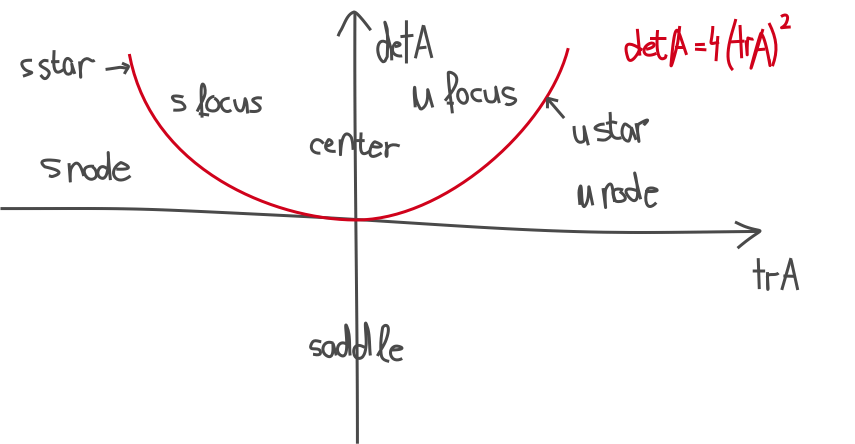
\includegraphics[scale=0.5]{graphic-nodes}
 
\subsection{Method of Lyapunov functions}

\marginpar{\textbf{Week 05}\\Tue, 13.11}

The idea of Lyapunov functions comes from physical systems that involve friction. Such systems do not converse energy, so that the total enery is a decreasing function of time. If we regard a pendulum, we see that the equilibrium point of such system lies at angle $0^\circ$ and $180^\circ$. The stability properties of both fixed point yield completely different behaviours. Linear stability analysis would linearise around the point corresponding to the angle $0^\circ$, and examine small perturbations of the angle. Lyapunov recognised that the reason for the stability of this fixed point has not much to do with small perturbations of the angle, but instead the sytem depends on its finite energy that keeps being dissipated. He developed a mathematical formalisation for scalar energly like functions that can be used to examine the behaviour of trajectories of the system.

\begin{framed}
	\textbf{Video Link:} \href{https://www.youtube.com/watch?v=jBAlzA0gYGk&feature=youtu.be}{General idea of Lyapunov functions by Professor Slotine at the MIT}
\end{framed}

Consider a scalar function $F: \mathbb R^n \to \mathbb R$ that is zero at some point $\mathbf{\tilde x}$ and positive elsewhere for a ball around zero. Such a function $F$ might be thought of an energy function. 

Let $\dot F$ denote the time derivative of $F$ along a trajectory $\Phi^t(\mathbf x)$ of the dynamical system. That means $\dot F$ describes the current rate of change of energy for a given moment $t$:
\[
	\dot F(t) \coloneqq \dot F(\Phi^t(\mathbf x)) \coloneqq \frac{d}{dt} F(\Phi^t(\mathbf x)), \quad \text{$\forall t \in \mathbb R$ and $\mathbf x$ is fixed}.
\]

If $\dot F$ is negative throughout the system trajectory (except at $\mathbf{\tilde x}$),  the energy function $F$ is strictly decreasing over time. Since $F(\mathbf{\tilde x}) = \mathbf 0$ is a lower bound, the energy of the system approaches zero, and any trajectory converges to this zero state. As we will see, we will call a function $F$ with these properties a \emph{Lyapunov function}. 

Let's further examine the time derivative $\dot F$. We will see that the rate at which energy varies along any system trajectory does not depend on time but only on the current position of the trajectory; that means we can write $F(t)$ as $F(\mathbf x)$. To see this, we derive $F(\Phi^t(\mathbf x))$ with respect to $t$ by the chain rule:
\[
	\dot F(\Phi^t(x)) = \frac{d}{dt}F(\Phi^t(\mathbf x)) = \frac{d}{d\Phi^t(\mathbf x)}F(\Phi^t(\mathbf x))  \cdot \frac{d}{dt}\Phi^t(\mathbf x) \overset{(!)}{=} \frac{d}{d\Phi^t}F(\Phi^t(\mathbf x)) \cdot f(\Phi^t(\mathbf x)), \quad \forall t \in \mathbb R.
\] 
The important step happens at $(!)$. For the system is autonomous, the derivative of $\Phi^t(\mathbf x)$ is $f(\Phi^t(\mathbf x))$; the derivative does not depend on $t$. Intuitively, the system knows where to go next, based on the information given by the current position. For any $t$, $\Phi^t(\mathbf x)$ identifies a particular position of the system, namely the position that the system arrives at when $\mathbf x$ is the starting point and time $t$ has passed. Let $\mathbf x$ denote this position, $\mathbf x \coloneqq \Phi^t(\mathbf x)$. Substitution for the time derivative $\dot F(\Phi^t(\mathbf x))$ yields:
\[
	\dot F(\mathbf x) = \frac{d}{d\mathbf x}F(\mathbf x) \cdot f(\mathbf x).
\]
To compare, if the system were nonautonomous: $\dot F(\Phi^t(\mathbf x)) =  \frac{d}{d\Phi^t}F(\Phi^t(\mathbf x)) \cdot f(\Phi^t(\mathbf x), t)$. The rate of change of energy for such a system hinges on its current position $\Phi^t(\mathbf x)$ and on how much time $t$ has passed since moving away from the starting point of the trajectory.

The derivative $\frac{d}{d\mathbf x} F(\mathbf x)$ is a row vector
\[
	\frac{d}{d\mathbf x}F(\mathbf x) = \begin{pmatrix}\frac{\partial}{\partial x_1}F(\mathbf x) & ... &  \frac{\partial}{\partial x_n}F(\mathbf x) \end{pmatrix} = \grad{F(\mathbf x)}^T.
\]
Thus, we obtain
\begin{framed}
\[
	\dot F(\mathbf x) = \grad{F(\mathbf x)}^T \cdot f(\mathbf x) = \sum^n_{k=1} \frac{\partial F}{\partial x_k}(\mathbf x) \cdot f_k(\mathbf x) = \mathcal L_fF(\mathbf x).
\]
\end{framed}

\begin{definition}[Lyapunov function]
Let $\mathbf{\tilde x}$ be a fixed point of $\Phi^t(\mathbf x)$. Let $\tilde M \subset \mathbb R^n$ be a neighborhood of $\tilde x$. We call a scalar function $F \in \mathcal C^{1}(\tilde M, \mathbb R)$ a \textbf{Lyapunov function} of $\Phi^t$ if
\begin{itemize}
	\item $F$ is \emph{positive definite} around $\mathbf{\tilde x}$, i.e. 
	\[
		F(\mathbf{\tilde x}) = 0 \quad \text{and} \quad F(\mathbf x) > 0, \text{ for all $\mathbf x \in \tilde M \setminus \{ \mathbf{\tilde x} \}$,}
	\]
	\item the time derivative of $F$ along any trajectory $\Phi^t(x)$ is \emph{negative semidefinite}, i.e.
	\[
		(\mathcal L_fF)(\mathbf x) \leq 0, \quad \text{for all $\mathbf x \in \tilde M$}.
	\]
\end{itemize}
$F$ is called a \textbf{strict Lyapunov function} if the derivative of $F$ along the system's trajectories is \emph{strictly negative definite}, i.e. $(\mathcal L_fF)(\mathbf x) < 0$ for all $\mathbf x \in \tilde M \setminus \{ \mathbf{\tilde x} \}$.
\end{definition}

\begin{theorem}[Lyapunov theorem]\label{theorem-lyapunov}
	Let $\mathbf{\tilde x}$ be a fixed point of $\Phi^t$.
	\begin{enumerate}
		\item If there exists a Lyapunov function $F$, then $\mathbf{\tilde x}$ is stable. \label{theorem:lyapunov-theorem-one}
		\item If there exists a strict Lyapunov function $F$, then $\mathbf{\tilde x}$ is asymptotically stable.
	\end{enumerate}
\end{theorem}

\begin{proof}[Proof of part one]
	We want to show that $\mathbf{\tilde x}$ is stable if there is a Lyapunov function $F$. 
	
	Let $\epsilon > 0$. We need to find a $\delta > 0$ such that $\Phi^t(B_{\delta}(\mathbf{\tilde x})) \subset B_{\epsilon}(\mathbf{\tilde x})$ for all $t \geq 0$. Define $m$ as the minimum of $F$ in the boundary of $B_{\epsilon}(\mathbf{\tilde x})$:
	\begin{align}\label{proof:lyapunov-theorem}
		m \coloneqq \min_{\substack{\mathbf x \in \partial  B_{\epsilon}(\mathbf{\tilde x})}} F(\mathbf x).
	\end{align}
	Note that the minimum $m$ is well defined because $F$ is continuous. That means, the boundary $\partial B_{\epsilon}(\mathbf{\tilde x})$ is not empty. Additionally, $m > 0$ because $F(\mathbf x) > 0$ for all $\mathbf{x} \in \tilde M \setminus \{ \mathbf{\tilde x} \}$. 
	
	Define the level set $U = \{ \mathbf x \in B_{\epsilon}(\mathbf{\tilde x}) : F(\mathbf x) < m \}$, which is not empty (due to $m > 0$ and $F(\mathbf{\tilde x}) = 0$) and open (due to the continuity of $F$). As $U$ is open, we find a ball with radius $\delta$ around $\mathbf{\tilde x}$ such that $B_{\delta}(\mathbf{\tilde x}) \subset U$. Note that $U$ may not be connected, yet we still manage to find such ball around $\mathbf{\tilde x}$. To conclude, every $\mathbf x \in B_{\delta}(\mathbf{\tilde x})$ satisfies: $F(\mathbf x) < m$.
	
	\begin{center}
		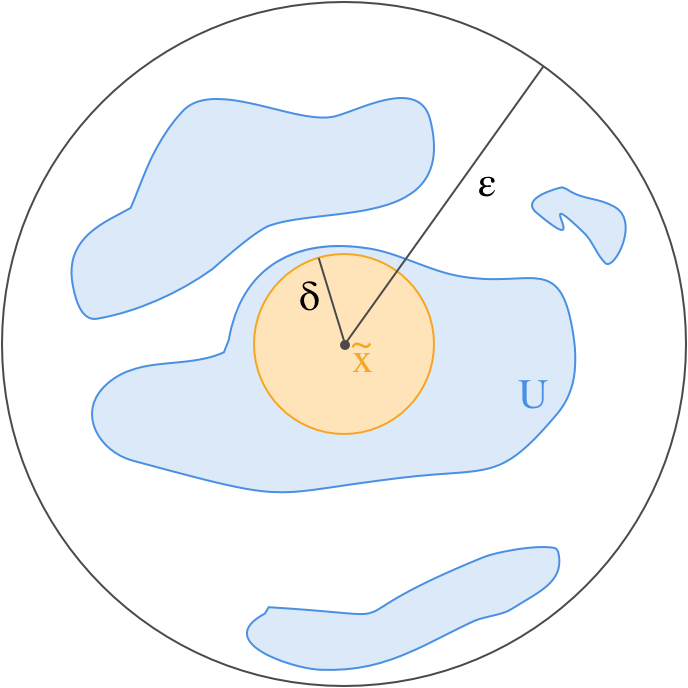
\includegraphics[scale=0.25]{lyapunov-theorem.png}
	\end{center}

	To prove stability of $\tilde x$, we show $\Phi^t(B_{\delta}(\tilde x)) \subset B_{\epsilon}(\tilde x)$ for all $t \geq 0$. 
	
	Assume, there exists a point $\mathbf x \in B_{\delta}(\mathbf{\tilde x})$ with  $t_1$ such that $\Phi^{t_1}(\mathbf x) \notin B_{\epsilon}(\mathbf{\tilde x})$. By continuity of the vector field $f$ we must have that at an earlier time $t_2$, it holds: $\Phi^{t_2}(\mathbf x) \in \partial B_{\epsilon}(\mathbf{\tilde x})$. Due to \eqref{proof:lyapunov-theorem}, we get 
	\[
		F(\Phi^{t_2}(\mathbf x)) \geq m.
	\]
	However, $\mathbf x \in B_{\delta}(\mathbf{\tilde x})$ and thus $F(\mathbf x) < m$. We know that $F$ is nonincreasing because of $\dot F(\Phi^t(\mathbf x)) \leq 0$ for all $t$ and therefore:
	\begin{align*}
		F(\Phi^{t_2}(\mathbf x)) - F(\mathbf x) &= \int^{t_2}_0 \frac{d}{ds}F(\Phi^s(\mathbf x)) ds \leq 0 \\
		&\Downarrow \\
			F(\Phi^{t_2}(\mathbf x))& \leq F(\mathbf x) < m.
	\end{align*}
	This is a contradiction, and thus it must hold: $\Phi^{t}(\mathbf x) \in B_{\epsilon}(\mathbf{\tilde x})$ for all $t$ and $\mathbf x \in B_{\delta}(\mathbf{\tilde x})$.
\end{proof}

\begin{proof}[Proof of part two]
	We want to show that $\mathbf{\tilde x }$ is asymptotically stable if $F$ is a strict Lyapunov function. The idea is to prove that $\lim\limits_{t \to \infty}F(\Phi^t(\mathbf x)) = 0$ for all $\mathbf x \in B_{\delta}(\mathbf{\tilde x})$. If that holds, it follows from  the continuity of $F$  
	\[
		F(\lim\limits_{t \to \infty} \Phi^t(\mathbf x)) = 0 \implies \lim\limits_{t \to \infty} \Phi^t(\mathbf x)= \mathbf 0,
	\]
	because $F(\mathbf x) = 0 \iff \mathbf x = \mathbf 0$. Thus, $\mathbf{\tilde x}$ is asymptotically stable, q.e.d.\\
	
	What remains is the proof of $\lim\limits_{t \to \infty}F(\Phi^t(\mathbf x)) = 0$. Since $\dot F(\Phi^t(\mathbf x))$ is strictly decreasing and $F(\Phi^t(\mathbf x)) \geq 0$ for all $t$, we know that $ \lim\limits_{t \to \infty} F(\Phi^t(\mathbf x)) = c$ for some $c \geq 0$. We show that $c = 0$ by contradiction. 
	
	Suppose $c > 0$. Let $S$ be the level set with $S \coloneqq \{ \mathbf x \in \mathbb R^n : F(\mathbf x) \leq c \}$. Let $B_{\alpha}(\mathbf{\tilde x}) \subset S$ and let $\Phi^t(\mathbf x)$ be a trajectory with $\mathbf x \in B_{\delta}(\mathbf{\tilde x})$. $F(\Phi^t(\mathbf x))$ strictly decreases monotically to $c$ and $F(\Phi^t(\mathbf{x})) > c$. Thus, $\Phi^t(\mathbf{x}) \notin B_{\alpha}(\tilde x)$ for all $t$. Additionally, $\Phi^t(\mathbf x)$ stays in $B_{\epsilon}(\mathbf{\tilde x})$ for any $t$ as we have shown in part one. Therefore, the trajectory moves within $\Vert \mathbf x - \mathbf{\tilde x} \Vert$ and we can define
	\[
		\gamma \coloneqq - \max_{\alpha\leq\Vert \mathbf x - \mathbf{\tilde x} \Vert \leq \epsilon} \dot F(\mathbf x).
	\]
	Clearly, $\gamma > 0$ because $\dot F(\mathbf x) < 0$. Observe that,
	\[
		F(\Phi^t(\mathbf x)) = F(\mathbf x) + \int^t_0 \dot F(\Phi^{\tau}(\mathbf x)) d\tau \leq F(\mathbf x) - t\gamma.
	\]
	For suffieciently large $t$, it would follow that $F(\Phi^t(\mathbf x)) < 0$ but that is a contradiction because $F$ is positive definite. Therefore, $c = 0$.
\end{proof}


\subsection{Lyapunov functions and linear systems}
\marginpar{\textbf{Week 05}\\Thu, 15.11}
Consider a linear, homogenous system
\[
	\begin{cases}
		\mathbf{\dot x} = A \mathbf x \\
		\mathbf x(0) = \mathbf x_0
	\end{cases}.
\]
We will provide a characterisation of a Lyapunov functions for linear systems. This result will later be needed to prove the Theorem of Poincaré-Lyapunov.

\begin{theorem}
	The fixed point $\mathbf{\tilde x} = 0$ of a linear system $\mathbf{\dot x} = A \mathbf x$ is asympototically stable if and only if for any positive definite symmetric matrix $Q \in \mathrm{GL}(n, \mathbb R)\footnote{space of all real invertible $n \times n$ matrices}$, there exists a positive definite symmetric matrix $P \in \mathrm{GL}(n, \mathbb R)$ that satisfies the matrix equation
	\[
		PA + A^TP = -Q.
	\]
\end{theorem}

\begin{proof}
``$\impliedby$'' We show if for any $Q$ there exists $P$ such that the matrix equation is satisfied, then $\mathbf{\tilde x} = 0$ is a fixed point. Consider the candidate Lyapunov function $F(\mathbf x) = \mathbf x^TP\mathbf x$. 

Prove that $F$ is indeed a Lyapunov function: $F$ is positive definite, i.e. $F(\mathbf x) > 0$ for all $\mathbf x \neq \mathbf{\tilde x}$ and $F(\mathbf{\tilde x}) = 0$. Note that $F$ is a dot product because $P$ is positive definite and symmetric.

Since $F$ is a Lyapunov function, we use the \hyperref[theorem-lyapunov]{theorem of Lyapunov} to show that $\mathbf{\tilde x}$ is asympotically stable. We need to show that $\mathcal L_fF(\mathbf x) < 0$ for all $\mathbf x \neq \mathbf{\tilde x}$.
\begin{align*}
	\mathcal L_fF(\mathbf x) &= \langle f(\mathbf x), \grad{F}(\mathbf x) \rangle \\
	&\Downarrow \tag{note: $\grad F(\mathbf x) = 2P \mathbf x$} \\
	&= 2 \langle A\mathbf x, P\mathbf x \rangle \\
	&= \langle \mathbf x, A^TP \mathbf x \rangle + \langle \mathbf x, PA \mathbf x \rangle \\
	&= \langle \mathbf x, (A^TP + PA) \mathbf x \rangle \\
	&= - \langle \mathbf x, Q\mathbf x \rangle <0 \tag{$Q$ is positive definite.}
\end{align*}

``$\implies$'' The fixed point $\mathbf{\tilde x} = 0$ is asymptotically stable. Thus all eigenvalues $\lambda_i$ have negative real part. We define the matrix $P$ as follows:
\[
	P \coloneqq \int^{\infty}_0 e^{A^Tt}Qe^{At}dt.
\]
The matrix $P$ is positive definite because $Q$ is positive definite and symmetric, and thus $e^{A^Tt}Qe^{At}$ defines a dot product in the vector space $\mathrm{Mat}_{n \times n}$. Additionally, the integral is converges because $A$ is the matrix corresponding to an asymptotically stable IVP, i.e. $e^{At} \to \mathbf 0_{n \times n}$ for $t \to \infty$. 

We substitute this into $PA + A^TP = -Q$ and see that the matrix equation is indeed satisfied. This step is omitted.
\end{proof}

Note that this proof explicitly gives a plan how to construct a Lyapunov function for linear systems if there are symmetric and positive definite matrices given with $PA + A^TP = -Q$.

\textit{... Proof of Lyapunov is missing, see raw notes from 15 November.}

\subsection{Topological equivalence of dynamical systems}

We try to find some kind of equivalence classes between dynamical systems. For that we need to specify when two dynamical systems are equivalent. Naturally, we expect that the phase portrait look qualitatively similar so that the number of fixed points or cycles are the same. We could also say that the phase portrait can be transformed into each other by a continuous map.

\begin{definition}\label{definition:topologically-conjugate}
	Two dynamical systems $(\Phi^t, \mathbb R, M_1)$ and $(\Psi^t, \mathbb R, M_2)$ are \textbf{topologically equivalent} if there exists a homeomorphism\footnote{A homeomorphism is a bijection that is continuous and whose inverse is continuous.} $\Lambda: M_1 \to M_2$ and a time-increasing function $\tau(t)\footnote{$\tau: \mathbb R\to \mathbb R, t \mapsto \tau(t)$ is continuous and monotically increasing. Such a map preserves the direction of time.}$ such that
	\[
		(\Lambda \circ \Phi^t)(\mathbf x) = (\Psi^{\tau(t)} \circ \Lambda)(\mathbf x), \quad \forall \mathbf x \in M_1, t \in \mathbb R.
	\]
		In other words, it is possible to find a map $\Lambda$  from one phase space to the other, and a map $\tau$ from one time in a phase space to time in the other, in such a way that the evolution is the same. Clearly topological equivalence maps fixed points to fixed points and periodic orbits to periodic orbits (though not necessarily of the same period). A stronger condition is \textbf{topologically conjugate}, that means time is preserved: $\tau = \mathrm{id_{\mathbb R}}$.
		\[
			(\Lambda \circ \Phi^t)(\mathbf x) = (\Psi^{t} \circ \Lambda)(\mathbf x), \quad \forall \mathbf x \in M_1, t \in \mathbb R.
		\]
	
	If $\Lambda$ is a diffeomorphism\footnote{A diffeomorphism a is continuously differentiable functions and its inverse is continuously differentiable as well.} of class $\mathcal C^k$, then $(\Phi^t, \mathbb R, M_1)$ and $(\Psi^t, \mathbb R, M_2)$ are called \textbf{$\mathcal C^k$-diffeomorphic}.
\end{definition}



Assume that $(\Phi^t, \mathbb R, M)$ with vector field $f$ and $(\Psi^t, \mathbb R, M)$ with vector field $g$ are $\mathcal C^k$-diffeomorphic with $\tau = \mathrm{id}_{\mathbb R}$. Then there exists a diffeomorphism $\Lambda \in \mathcal C^k(M,M)$ such that
\[
	\Lambda(\Phi^t(\mathbf x)) = \Psi^t(\Lambda(\mathbf x)), \quad \forall \mathbf x \in M.
\]
Differentiating with respect to $t$ at $t=0$ yields
\begin{align*}
	D\Lambda(\mathbf x)\cdot f(\mathbf x) &= g(\Lambda(\mathbf x)) \\
	&\Downarrow \\
	f(\mathbf x) &= (D\Lambda(\mathbf x))^{-1}g(\Lambda(\mathbf x)).
\end{align*}
Note that $D\Lambda(\mathbf x)$ is the Jacobian matrix of $\Lambda$. Two diffeomorphic systems are practically identical and can be viewed as the same system using different coordinates.

\begin{example}
	Consider the three dynamical systems
	\[
		\begin{cases}
			\dot x_1 = -2x_1 \\
			\dot x_2 = -2x_2
		\end{cases} 
		\begin{cases}
			\dot x_1 = -2x_1 +x_2\\
			\dot x_2 = -x_1-2x_2
		\end{cases}
		\begin{cases}
			\dot x_1 = -2x_1 \\
			\dot x_2 = x_1-2x_2
		\end{cases}
	\]
	The eigenvalues of the corresponding matrices are
	\[
		\lambda_{1,2} = -2 \quad \lambda_{1,2} = -2 \pm i, \quad \lambda_{1,2} = -2.
	\]
	The fixed point $(0,0)$ is asymptotically stable in all three cases because all eigenvalues have positive real part.
	
	The phase portraits of the system are depicted by the graphics below:
	
	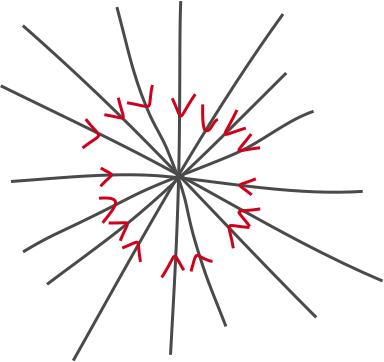
\includegraphics[width=5cm]{phase_portrait_example1.png}
	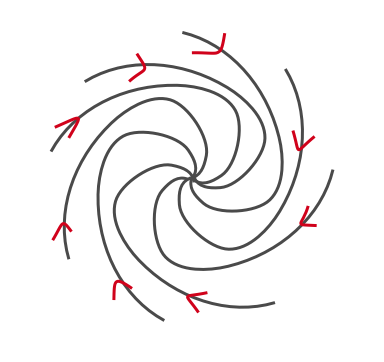
\includegraphics[width=5cm]{phase_portrait_example2.png}
	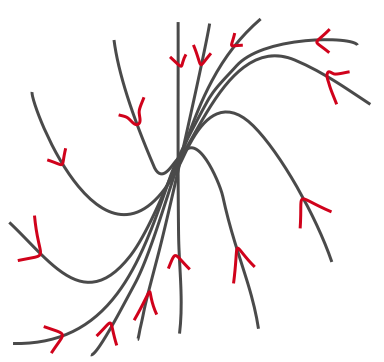
\includegraphics[width=5cm]{phase_portrait_example3.png}
	
	We rewrite the systems in polar coordinates. The first two systems expressed in polar coordinates are
	\[
		\begin{cases}
			\dot r = -2r \\
			\dot \theta = 0
		\end{cases} \quad \text{and} \quad 
		\begin{cases}
			\dot s = -2s \\
			\dot \varphi = -1
		\end{cases}
	\]
	The behaviour of the systems expressed in polar coordinates match the pictures. The radius is decreasing. For the first system the angle remains constant while for the second the angle constantly decreases, which results in rotation to the right.
	
	System one and two are topologically conjugate for the homeomorphism $\Lambda: (s,\varphi) \mapsto (r, \theta)$ maps the phase spaces from system one to two and preserves time:
	\[
		\Lambda(s, \varphi) = (s, \varphi - \frac{1}{2}\ln s).
	\]
	To show that this is indeed the corresponding homeomorphism integrate both system to obtain the solution of the ODEs
	\[
		\Phi^t_1(r, \theta) = (re^{-2t}, \theta) \quad \text{and} \quad \Phi^t_2(s, \varphi) = (se^{-2t}, \varphi-t)
	\]
	and check
	\begin{align*}
		\Lambda(\Phi^t_2(s, \varphi)) 
		&= \Lambda(se^{-2t}, \varphi -t) \\
		&= (se^{-2t}, \varphi - t- \frac{1}{2}\ln(se^{-2t})) \\
		&= (se^{-2t}, \varphi - t- \frac{1}{2}\ln(s) + t) \\
		&= (se^{-2t}, \varphi - \frac{1}{2}\ln(s))\\
		&= \Phi^t_1(s, \varphi - \frac{1}{2} \ln(s)) \\
		&= \Phi^t_1(\Lambda(s, \varphi)).
	\end{align*}
	Therefore, system one and two are topologically conjugate.
	
	The first and third system are topologically conjugate. The homeomorphism is 
	\[
		\Lambda: (x_1,x_2) \mapsto (x_1,x_2 - \frac{x_1}{2}\ln(|x_1|).
	\]
	First, obtain the explicit solutions for system one and system three. The solutions are
	\[
		\Phi^t_1(x_1,x_2) = \begin{pmatrix}x_1e^{-2t}\\ x_2e^{-2t}\end{pmatrix} \quad \text{and} \quad \Phi^t_3(x_1,x_2) = \begin{pmatrix}x_1e^{-2t}\\ x_1te^{-2t} + x_2e^{-2t}\end{pmatrix}.
	\]
	For the solution of the third system, we calculated the Jordan normalform which is 
	\[
		A_3 = \begin{pmatrix}
			-2 & 0 \\ 1 & -2
		\end{pmatrix} = \begin{pmatrix}
		0 & 1 \\ 1 & 0
		\end{pmatrix}
		\begin{pmatrix}
		-2 & 1 \\ 0 & -2
		\end{pmatrix}\begin{pmatrix}
		0 & 1 \\ 1 & 0
		\end{pmatrix}.
	\]
	Then compute the matrix exponential $e^{A_3t} = \begin{pmatrix}
	0 & 1 \\ 1 & 0
	\end{pmatrix}e^{-2t}\begin{pmatrix}
		1 & t \\ 0 & 1
	\end{pmatrix}\begin{pmatrix}
	0 & 1 \\ 1 & 0
	\end{pmatrix} = \begin{pmatrix}
		e^{-2t} & 0 \\ te^{-2t} & e^{-2t}
	\end{pmatrix}$. Finally, the solution is given by $\Phi^t_3(x_1,x_2) = e^{At}\begin{pmatrix}
		x_1 \\ x_2
	\end{pmatrix}$.
	
	Now when we have both solutions, we just need to validate the formula given by Definition \ref{definition:topologically-conjugate}, which we will omit.
\end{example}

The following theorem justifies the approach to examine a linearised version of a \underline{hyperbolic} nonlinear system in order to analyse the behaviour of the nonlinear system around the equilibrium.

\begin{framed}
\begin{theorem}[Hartman-Grobman]
	Consider a hyperbolic nonlinear IVP in $M \subset \mathbb R^n$:
	\[
		\begin{cases}
			\mathbf{\dot x} = A \mathbf x + h(\mathbf x) \\
			\mathbf{x} (0) = x_0 
		\end{cases} \quad \text{with} \quad h \in \mathcal C^1(M, \mathbb R^n), h(\mathbf 0) = \mathbf 0 \text{ and } \frac{d h}{d \mathbf x} \Bigg\vert_{\mathbf x = \mathbf 0} = \mathbf 0.
	\]
	For a neighborhood $\tilde M$ of the hyperbolic fixed point $\mathbf{\tilde x} = \mathbf 0$, the nonlinear system is locally topologically conjugate to the linearised system.
	
	Precisely, if $\Phi^t$ is the flow of the nonlinear system, then there exists a homeomorphism $\Lambda$ such that
	\[
		\Lambda(e^{At}\mathbf x) = \Phi^t(\Lambda(\mathbf x)), \quad \forall \mathbf x \in \tilde M, t \in \mathbb R.
	\]
\end{theorem}
\end{framed}

\begin{example}[Hyperbolic fixed point]
	Consider the nonlinear IVP in $\mathbb R^2$:
	\[
		\begin{cases}
		\dot x_1 = 2x_1 + x_2^2 \\
		\dot x_2 = x_2 \\
		x_1(0), x_2(0) \in \mathbb R
		\end{cases}.
	\]
	The orbits of the nonlinear system are given by the curves
	\[
		x_1 = x_2^2 (\alpha + \log|x_2|), \quad \alpha \in \mathbb R.
	\]
	The parameter $\alpha$ depends on the initial conditions $(x_1(0), x_2(0))$. The linearisation of the nonlinear system around the fixed point $(0,0)$ reads as
	\begin{align*}
		\frac{\partial f}{\partial x_i}(0,0) &= \begin{pmatrix}
			2 - x_2^2 & 2x_1-2x_2 \\
			0 & 1
		\end{pmatrix} \Bigg \vert_{\mathbf x =(0,0)} \\
		&\Downarrow  \\
		\begin{pmatrix}
			\dot x_1 \\ \dot x_2
		\end{pmatrix} &= 
		\begin{pmatrix}
			2 & 0 \\ 0 & 1
		\end{pmatrix} \begin{pmatrix}
		x_1 \\ x_2
		\end{pmatrix}.
	\end{align*}
	We see that the system is hyperbolic since all eigenvalues have positive real part (the eigenvalues are $1$ and $2$). Additionally, the linear system is unstable and after Hartman-Grobman the nonlinear system is unstable, too. The orbits of the linearised system are given by
	\[
		x_1 = \alpha x_2^2, \quad \alpha \in \mathbb R.
	\]
	\textit{Phase portrait of the nonlinear (left) and linear (right) system:}
	
	\includegraphics*[width=7.0cm]{topo_conjugate_nonlinear.png}
	\includegraphics*[width=7.0cm]{topo_conjugate.png}
	
\end{example}

\marginpar{\textbf{Week 06}\\Tue, 20.11}

\textit{one example missing...}

\begin{example}[Nonhyperbolic fixed point]
	Consider the ODE
	\[
		\begin{cases}
			\dot x_1 = x_2 + \lambda x_1(x_1^2+x_2^2)  \\
			\dot x_2 = -x_1 + \lambda x_2(x_1^2+x_2^2)
		\end{cases}.
	\]
	$(0,0)$ is a fixed point. The linearisation $\mathbf{\dot y} = A \mathbf y$ at $(0,0)$ is given by
	\[
		A = Df(0,0) = \begin{pmatrix}
			0 & 1 \\ -1 & 0
		\end{pmatrix} \quad \text{with eigenvalues} \quad \lambda_{1,2}= \pm i.
	\]
	Since at least one eigenvalue has zero real part, the fixed point $(0,0)$ is not hyperbolic and the theorem of Grobman-Hartman is \emph{not} applicable. To examine the stability behaviour of the nonlinear system we need to find a Lyapunov function instead. Therefore, we write system in polar coordinates where $r$ denotes the radius: $r^2(x_1,x_2) = x_1^2 + x_2^2$. Clearly, the system converges to zero if the radius vanishes with the time. The angle $\theta$ has no influence on the stability behaviour.
	
	To be a Lyapunov function $r$ must be positive definite. This is true since $r(0,0) = 0$ and $r(x_1,x_2) > 0$ for all $(x_1,x_2) \neq \mathbf 0$. Now we have to validate that the time derivative of $r$ along any system trajectory $x_1^2 + x_2^2$ is negative, i.e. $\frac{d}{dt}r^2(x_1, x_2) < 0$.
	\begin{align*}
		(r^2(x_1,x_2))^{\boldsymbol{\cdot}} \overset{(*)}{=} 2r(x_1,x_2)\dot r(x_1,x_2) &= (x_1^2 + x_2^2)^{\boldsymbol{\cdot}}\\
		 &= 2x_1\dot x_1 + 2x_2\dot x_2 \\
		&= 2x_1(x_2 + \lambda x_1r^2(x_1,x_2))+2x_2(-x_1 + \lambda x_2 r^2(x_1,x_2)) \\
		&\overset{(**)}{=} 2\lambda r^4(x_1,x_2)
	\end{align*}
	Compare $(*)$ and $(**)$ and rearrange the equation by dividing with $2r(x_1,x_2)$:
	\begin{align*}
		\dot r(x_1,x_2) = \lambda r^3(x_1,x_2) &= \lambda\sqrt{(x_1^2 + x_2^2)^3} \\
		&\Downarrow \text{if $\lambda$ is negative} \\
		&< 0.
	\end{align*}
	Therefore, if $\lambda < 0$ we have found a strict Lyapunov function for the trivial fixed point which means that the $(0,0)$ is asymptotically stable. If $\lambda > 0$ the radius grows with the time and thus the system is unstable in $(0,0)$.
	
	\begin{center}
		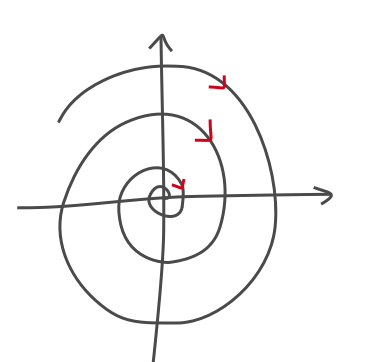
\includegraphics[width=5cm]{nonhyperbolic_stable_example}
	\end{center}
\end{example}

\subsection{Fixed points in dynamical systems with discrete time} \label{chap:fixed-points-dynamical-systems}
Consider a map $\Phi: X \to X$ generating a discrete dynamical system $(\Phi)_{n \in \mathbb Z}$.
\begin{framed}
	\[
		\text{$\mathbf x_0$ is a fixed point if and only if $\mathbf x_0 = \Phi(\mathbf x_0)$}.
	\]
\end{framed}
Stability is defined exactly as for continuous time system.

We linearise the discrete system $\mathbf x_{n+1}  = \Phi(\mathbf x_n)$ around the fixed point $\mathbf x_0$
\[
	\mathbf x = \mathbf x_0 + \mathbf y \quad \text{with a linear map $\mathbf y$}.
\]
A step is described by $\mathbf x_{n+1} = \Phi(\mathbf x_n)$ leading to 
\begin{align*}
	\mathbf x_0 + \mathbf y_{n+1} &= \Phi(\mathbf x_0 + \mathbf y_n)\\
	&\Downarrow \text{Taylor expansion up to the first order} \\
	&\approx \Phi(\mathbf x_0) + d \Phi(\mathbf x_0)\mathbf y_n \\
	&= \mathbf x_0 + d \Phi(\mathbf x_0)\mathbf y_n \\
	&\Downarrow \\
	\mathbf{y}_{n+1} &= d \Phi(\mathbf x_0)\mathbf y_n.
\end{align*}
The linearised discrete system is obtained by
\begin{framed}
\[
	\mathbf y_{n+1} = B\mathbf y_n, \quad B = d \Phi(\mathbf x_0), \quad  \text{ $B$ is the Jacobi matrix of $\Phi$}.
\]
\end{framed}
Compare this with a linearised continuous system
\[
	\mathbf{\dot y} = A \mathbf y, \quad A = df(\mathbf x_0).
\]
Note that a solution $\mathbf y_n$ of the linear discrete system is given by $\mathbf y_n = B^n \mathbf y_0$. If $B$ is a diagonalisable, i.e. $B = U\mathrm{diag}(\mu_1,...,\mu_d)U^{-1}$, then $B^n = U \mathrm{diag}(\mu_1^n,...,\mu_d^n) U^{-1}$.

Observe
\begin{itemize}
	\item if $|\mu_i| < 1$ then $\lim_{n \to \infty}\mu_i^n = 0$
	\item if $|\mu_i| > 1$ then $\lim_{n \to \infty}\mu_i^n = \infty$
	\item if $|\mu_i| = 1$ then $|\mu_i|^n = 1$.
\end{itemize}

{\def\arraystretch{2}\tabcolsep=6pt

\begin{tabular}{m{4cm}|m{4cm}|m{4cm}}
	& Continuous time & Discrete time \\ \hline
	Dynamical system &        $\mathbf{\dot x} = f(\mathbf x)$         &      $\mathbf x_{n+1} = \Phi(\mathbf x_n)$         \\
	Fixed point &    $f(\mathbf x_0) = \mathbf 0$             &     $\mathbf x_0 = \Phi(\mathbf x_0)$          \\
	Linearisation around a fixed point &      $\begin{cases}
		\mathbf{\dot y} = A \mathbf y \\ A = df(\mathbf x_0)
	\end{cases}$           &        $\begin{cases}
		\mathbf y_{n+1} = B \mathbf y_n \\ B = d\Phi(\mathbf x_0)
	\end{cases}$       \\
	Solution of the linearised system &      $\mathbf y = e^{At}\mathbf y_0$           &      $\mathbf y_n = B^n \mathbf y_0$         \\
	Asymptotical stability&       All eigenvalues have negative real part          &       All eigenvalues have absolute value smaller one        \\
	Instablity &      At least one eigenvalue has positive real part           &        At least one eigenvalue has absolute value bigger than one       \\
	Contributions of eigenvalues to solutions of the linearised system & $e^{\lambda_it}$& $\mu_i^n$
\end{tabular}



\section{Stability of periodic solutions}

Periodic solutions are flows whose orbits are closed trajectories. While pariticular points on periodic orbits $\mathbf x(t_0)$ are no fixed points and therefore it does not make sense to talk about stability of single points, we can consider the stability of the whole orbit as an invariant set.

\subsection{Definition and examples}
Before we introduce the notion of stability of periodic orbits, let's examine one example to get an intuitive grasping of the concept.
\begin{example}
	Consider the continuous system:
	\begin{align*}
		\begin{cases}
			\dot x_1 = -x_2 +x_1(1-x_1^2-x_2^2) \\
			\dot x_2 = x_1 + x_2(1-x_1^2-x_2^2)
		\end{cases}.
	\end{align*}
	Transform into polar coordinates.
	\[
		\begin{cases}
			x_1 = r\cos(\varphi) \\
			x_2 = r \sin(\varphi)
		\end{cases}
	\]
	Set $\rho \coloneqq r^2 = x_1^2 +x_2^2$ and try to find the constraint of $\rho$.
	\begin{align*}
		\dot \rho = (x_1^2 + x_2^2)^{\boldsymbol{\cdot}} = 2x_1\dot x_1 + 2x_2\dot x_2 &= 2x_1(-x_2 + x_1(1-\rho)) + 2x_2(x_1 + x_2(1- \rho)) \\
		&=2(x_1^2 + x_2^2)(1- \rho) \\
		&= 2\rho(1-\rho).
	\end{align*}
	Separation of variables results in
	\[
		\frac{d\rho}{\rho(1-\rho)} = 2 dt \iff \frac{d\rho}{\rho} + \frac{d\rho}{1-\rho} = 2dt \iff \ln(\frac{\rho}{1-\rho}) = 2t + \mathrm{const} \iff \frac{\rho}{1-\rho} = \mathrm{const} \cdot e^{2t}.
	\]
	Depending on the sign of the constant we get
	\[
		\frac{\rho}{1-\rho} = \pm e^{2(t - t_0)}.
	\]
	$t_0$ is a parameter which is to determined such that $\rho(0) = \rho_0$. The angle of the coordinates is given by $\varphi = \arctan(\frac{x_2}{x_1})$. Remember that $\frac{d}{dx}\arctan(x) = \frac{1}{1+x^2}$. Thus
	\begin{align*}
		\dot \varphi = (\arctan(\frac{x_2}{x_1}))^{\boldsymbol\cdot} = \frac{\frac{\dot x_2 x_1 - \dot x_1 x_2}{x_1^2}}{1 + \frac{x_2^2}{x_1^2}} &= \frac{\dot x_2 x_1 - \dot x_1 x_2}{x_1^2+x_2^2} \\
		&= \frac{x_1(x_1 + x_2(1- \rho)) - x_2(-x_2 +  x_1(1- \rho))}{x_1^2+x_2^2} \\
		&= \frac{x_1^2 + x_2^2}{x_1^2 + x_2^2} \\
		&= 1 \\
		&\Downarrow \\
		\varphi(t)&  = t + \varphi_0 .
	\end{align*}
	For the evolution of $\rho$: If the initial value $\rho(0)$ lies between $0 < \rho(0) < 1$ then $\frac{\rho(0)}{1-\rho(0)} > 0$ so that we must take the positive sign of $\frac{\rho(t)}{1-\rho(t)} = e^{2(t-t_0)}$. Thus 
	\[
		\rho(t) = \frac{e^{2(t-t_0)}}{e^{2(t-t_0)} + 1} \to \begin{cases}
			1, \quad t \to \infty \\
			0, \quad t \to - \infty
		\end{cases}
	\]
	If $\rho > 1$ then $\frac{\rho(0)}{1-\rho(0)} <0$ so that $\frac{\rho(t)}{1-\rho(t)} = -e^{2(t-t_0)}$. 
	\[
		\rho(t) = \frac{e^{2(t-t_0)}}{e^{2(t-t_0)} -1} \to \begin{cases}
			1, \quad & t \to \infty \\
			\infty, \quad &t \searrow t_0
		\end{cases}
	\]
	\begin{center}
		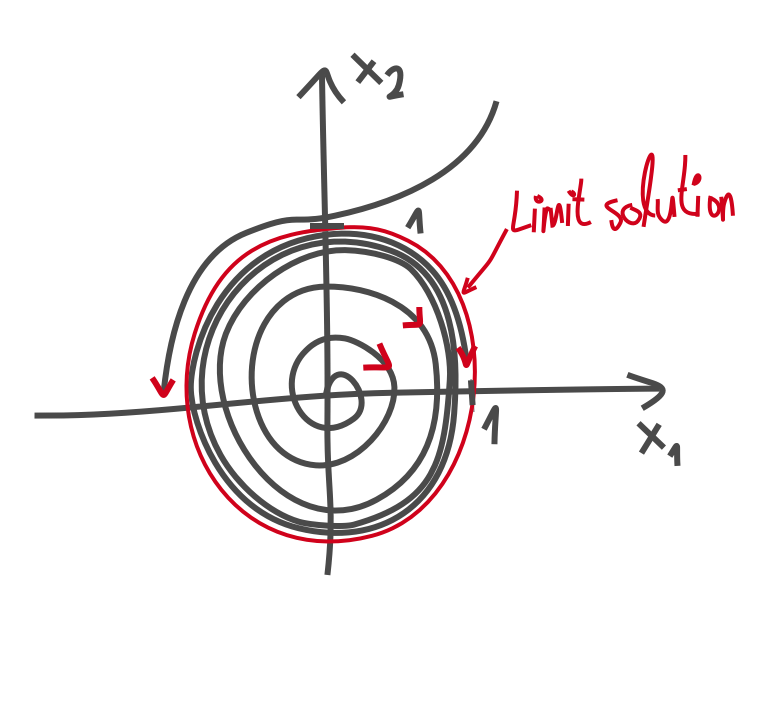
\includegraphics[width=7cm]{limit_solution.png}
	\end{center}
The limit solution is a circle with radius one. It is asymptotically stable. Therefore the isolated periodic solution is $\rho(t) \equiv 1, \varphi(t) = t + \varphi_0$. This is equivalent to
\[
	\begin{cases}
		x(t) = \cos(t+\varphi_0) \\
		y(t) = \sin(t + \varphi_0)
	\end{cases}
\]
All other solutions approach this solution as $t$ goes to infinity.
\end{example}

\begin{definition}[Stability of periodic solutions]
	Let $\mathbf x_0(t)$ be a $T$-periodic solution of $\mathbf{\dot x} = f(\mathbf x)$ with trajectory $\gamma = \{ \mathbf x : \mathbf x = \mathbf x_0(t), t \in \mathbb R \}$. It is called \textbf{asymptotically stable} if the following requirements hold true
	\begin{itemize}
		\item $\forall \epsilon >0, \exists \delta > 0, \forall \mathbf y \in B_{\delta}(\gamma): \Phi^t(\mathbf y) \in B_{\epsilon}(\gamma), \quad \forall t \in \mathbb R$,
		\item $\exists \delta > 0, \forall \mathbf y \in B_{\delta}(\gamma): \mathrm{dist}(\Phi^t(\mathbf y), \gamma) = \min\limits_{\mathbf x_0 \in \gamma} |\Phi^t(\mathbf y) - \mathbf x_0| \to 0$ for $t \to \infty$.
	\end{itemize}
	We say that the asymptotic stability takes place with an \textbf{asymptotic phase} $c \in \mathbb R$ if $$\exists \delta > 0, \forall \mathbf y \in B_{\delta}(\gamma): |\Phi^t(\mathbf y) - \mathbf x_0(t+c)| \to 0 \quad \text{for} \quad t \to \infty.$$
\end{definition}

\marginpar{\textbf{Week 06}\\Thu, 22.11}

\begin{example}
	Consider the dynamical system examined from last week
	\begin{align}\label{chapter:periodic-solutions-model-example}
		\begin{cases}
		\dot x_1 = -x_2 +x_1(1-x_1^2-x_2^2) \\
		\dot x_2 = x_1 + x_2(1-x_1^2-x_2^2)
		\end{cases}.
	\end{align}
	We know that $\mathbf x(t) = (\cos t, \sin t)$ is a solution of this ODE. The period is $T = 2\pi$ as $\mathbf x(t + T) = \mathbf x(t)$ for all $t \in \mathbb R$. We want to linearise the nonlinear system along the periodic solution and see how the periodicity is reflected in the linear system. The linear system is $\mathbf{\dot y} = A(t) \mathbf y$ with $A(t) = \frac{\partial f}{\partial x}f(\mathbf x(t))$.
	\begin{align*}
		\begin{pmatrix}
			{\dot y_1} \\
			{\dot y_2}
		\end{pmatrix} &= \left.
		\begin{pmatrix}
			1-9x_1^2 & -1-2x_1x_2 \\
			1-2x_1x_2 & 1 - x_1^2-3x_2^2
		\end{pmatrix} \right \vert_{(x_1,x_2) = (\cos t, \sin t)} \begin{pmatrix}
			y_1 \\ y_2
		\end{pmatrix} \\
		&= \underbrace{\begin{pmatrix}
			-2\cos^2t & -1-2\cos t \sin t \\ 
			1-2 \cos t \sin t & -2 \sin^2t
		\end{pmatrix}}_{=A(t)} \begin{pmatrix}
		y_1 \\ y_2
		\end{pmatrix}.
	\end{align*}
	The matrix $A(t) $ is $2\pi$ periodic (accidentically, it is even $\pi$-periodic but we will ignore this). Thus $A(t + 2\pi) = A(t)$ for all real $t$.
	
	Imagine we do not know that the solution $\mathbf x(t)$ is $2\pi$ periodic but we do know that the linearised system is $2\pi$ periodic. Can we interfere periodicity properties for the nonlinear system? We could if we know that the linearised system is hyperbolic for at least one point along the solution. This is great because we only need to find one hyperbolic solution along $A(t)$, i.e. find $t_0$ such that all eigenvalues of $A(t_0)$ have nonnegative real part. If we would find such $t_0$, we can conclude that the nonlinear system and linear system are topologically conjugate after the theorem of Hartman-Grobman. That means the nonlinear system is periodic, for $x(t_0 + T) = x_{(t_0)}$ implies $x(t + T) = x(t)$ for all $t \in \mathbb R$ (we have shown in an exercise sheet that if a solution is at one particular point periodic, it is periodic everywhere). How can find a $t_0$ such that all eigenvalues of $A(t_0)$ have nonzero real parts? We use the mean value theorem for integrals
	\[
		\frac{1}{2\pi} \int^{2\pi}_0 A(t) dt = \begin{pmatrix}-1 & -1 \\ 1 & -1\end{pmatrix}  = A(t_0), \quad t_0 \in (0, 2\pi).
	\]
	$A(t_0)$ is hyperbolic for the characteristic polynomial is $(\lambda + 1)^2=0$ and the eigenvalues are $\lambda_{1,2} = -1 \pm i$. Thus the nonlinear system is $2\pi$-periodic.
\end{example}

\subsection{Floquet theory of linear differential equations with periodic coefficients}

\subsubsection{Homogeneous systems}
Consider a periodic homogeneous linear ODE in $\mathbb R^n$: 
\[
	\mathbf{\dot x} = A(t) \mathbf x, \quad A:\mathbb R \to \mathrm{Mat}_{n \times n} \text{ is continuous and $T$-periodic}\footnote{The matrix function $A(t)$ is called $T$-periodic if $A(t + T) = A(t)$ for all $t \in \mathbb R$}.
\] 

\begin{theorem}[Theorem of Floquet]
	Every fundamental matrix $X(t)$ of $\dot X = A(t) X$ can be represented in the form
	\[
		X(t) = P(t) e^{tR}
	\]
	where $P(t)$ is a $T$-periodic matrix-valued function and $R \in \mathrm{Mat}_{n \times n}$.
\end{theorem}

\begin{proof}
	Take any fundamental matrix $X(t)$ and consider the time-shifted matrix solution $Z(t) \coloneqq X(t+ T)$ with period $T \in \mathbb R$. We show that $Z(t)$ is also a fundamental matrix:
	\[
		\dot Z(t) = \dot X (t+T) = A(t+T)X(t+T) = A(t)X(t+T)= A(t)Z(t).
	\]
	By \hyperref[theorem:fundamental-matrix-constant]{Theorem \ref{theorem:fundamental-matrix-constant}} we get that $X(t+T) = X(t) C$ for an invertible matrix $C$.
	
	\textbf{Claim:} Any non-degenerate $C \in \mathrm{Mat}_{n \times n}(\mathbb R)$ has a \textbf{matrix logartihm} $S \in \mathrm{Mat}_{n \times n}(\mathbb C)$ such that $e^S = C$. We prove the claim: If $C$ is non-degenerate and diagonalisable, then $C = U \Lambda U^{-1}$ with $\Lambda = \mathrm{diag}(\lambda_1,...,\lambda_n)$ and $\lambda_i \neq 0$ for all $i=1,...,n$. Set 
	\[
		S \coloneqq U \mathrm{diag}(\ln(\lambda_1), ..., \ln(\lambda_n))U^{-1}.
	\] 
	If $C$ is non-degenerate and not diagonalisable, then it has at least a Jordan normal form: $C = U\mathrm{diag}(J_1,...,J_k)U^{-1}$ where $J_i = \lambda I + N$ are Jordan blocks. Set
	\[
		S \coloneqq U \mathrm{diag}(\ln(J_1),...,\ln(J_k)) U^{-1}
	\]
	where
	\[
		\ln(\lambda I + N) = \ln(\lambda)I + \ln(I + \frac{1}{\lambda}N) = \ln(\lambda) I +\underbrace{ \sum^{\infty}_{j=1}\frac{(-1)^{j-1}}{j}(\frac{1}{\lambda}N)^j}_{< \infty \text{ because $N$ is nilpotent}}.
	\]
	This proves the claim of the existence of a matrix logarithm.
	
	Having proved the claim, we return back to the proof of the theorem of Floquet. We set
	\begin{framed}
	\[
		R \coloneqq \frac{1}{T}\ln C, \quad P(t) \coloneqq X(t)e^{-tR}.
	\]
	\end{framed}
	Check that $P$ is a $T$-periodic matrix function, i.e. $P(t+T) = P(t)$ holds true for all $t \in \mathbb R$. Indeed 
	\begin{align*}
		P(t+T) = X(t+T)e^{(-t+T)R} = X(t+T)e^{-TR-tR} &= X(t+T)e^{-TR}e^{-tR} \\
		&\Downarrow \text{note: $e^{-TR} = e^{-\ln C} = C^{-1}$}\\
		&= X(t+T)C^{-1}e^{-tR}\\
		&\Downarrow \text{note: $X(t+T)=X(t)C$}\\
		&= X(t)e^{-tR} \\
		&= P(t).
	\end{align*}
	Check that $P(t)e^{tR} = X(t)e^{-tR}e^{tR} = X(t)$. The theorem of Floquet is proved.
\end{proof}

Note that the proof gives us a formula on how to chose $R$ and $P(t)$. Besides, we showed that $X(t+T)$ is a fundamental solution. 

\begin{definition}
	A matrix $C$ is called a \textbf{monodromy matrix} for a fundamental matrix $X(t)$ if $X(t+T) = X(t)C$ for all $t \in \mathbb R$. Eigenvalues of $C$ are called \textbf{Floquet multipliers}.
\end{definition}

\begin{theorem}
	Any other monodromy matrix $\tilde C$ for any other fundamental matrix $\tilde X(t)$ is conjugate to the monodromy matrix $C$ of $X(t)$. Thus, Floquet multipliers do not depend on the choice of solution.
\end{theorem}

\begin{proof}
	Let $\tilde X$ be any other fundamental matrix and let $\tilde C$ be its monodromy matrix, i.e. $\tilde X(t+T) = \tilde X(t) \tilde C$. After \hyperref[theorem:fundamental-matrix-constant]{Theorem \ref{theorem:fundamental-matrix-constant}}, there exists $D$ such that $\tilde X(t) = X(t)D$. We get
	\[
		\tilde X(t+T) = X(t+T)D=X(t)CD = \tilde X(t)D^{-1}CD \implies \tilde C = D^{-1}CD.
	\]
	The eigenvalues of $C$ and $\tilde C$ are equal.
\end{proof}

\begin{theorem}
	A complex value $\mu \in \mathbb C$ is a Floquet multiplier for $\mathbf{\dot x} = A(t) \mathbf x$ if and only if there exists a nontrivial solution $\mathbf x(t)$ such that $\mathbf x(t+T) = \mu \mathbf x(t)$. Such solutions are called \textbf{Floquet solutions}.
\end{theorem}

\begin{proof}
	$\mu$ is a multiplier if and only if $C\mathbf u = \mu \mathbf u$ for eigenvectors $\mathbf u \neq \mathbf 0$. Set $\mathbf x(t) \coloneqq X(t) \mathbf u$. We have
	\[
		\mathbf x(t+T) = X(t+T)\mathbf u = X(t)C\mathbf u = \mu X(t) \mathbf u = \mu \mathbf x(t).
	\]
\end{proof}

\begin{collorary}\label{chapter:floquet-t-periodic-collorary}
	The system $\mathbf{\dot x} = A(t) \mathbf x$ with a $T$-periodic matrix function $A(t)$ has a $T$-periodic solution if and only if $1$ is a Floquet multiplier.
\end{collorary}

It is very difficult to analytically find multipliers for a given system; it is an easy task to find it numerically. The \hyperref[formula:liouville]{formula by Liouville} gives additional information about the Floquet multipliers:
\begin{align*}
	\det X(T) &= \det X(0) e^{\int^T_0 \tr (A(z)) dz} \\
	X(T+t) = X(t)C  &\Downarrow \\
	\det (X(0) \cdot C) &= \det X(0) e^{\int^T_0 \tr (A(z)) dz} \\
	&\Downarrow \text{divide by $\det X(0)$}\\
		\mu_1\cdot ... \cdot \mu_n = \det C &= e^{\int^T_0 \tr A(z) dz}.	
\end{align*}

\subsubsection{Nonhomogenous systems}
	Consider a non-homogeneous system
\begin{align*}
\mathbf{\dot x} = A(t)\mathbf x + \mathbf b(t), \quad \text{$A(t)$ and $\mathbf b(t)$ are $T$-periodic.}
\end{align*}
\begin{theorem}\label{chapter:floquet-non-homo-periodic-solution}
A solution $\mathbf x(t)$ of this system is $T$-periodic if and only if $\mathbf x(0) = \mathbf x(T)$.
\end{theorem}
\begin{proof}
 The necessity is obvious: if a solution $\mathbf x(t)$ is periodic with period $T	$, then $\mathbf x(0) = \mathbf x(0 + T) = \mathbf x(T)$. To show sufficiency: Let $\mathbf x(t)$ be a solution of the non-homogeneous system with $\mathbf x(0) = \mathbf x(T)$. We need to show that $\mathbf x(t)$ is $T$-periodic. Consider $\mathbf y(t) \coloneqq \mathbf x(t+T)$ which solves the non-homogeneous system:
\begin{align*}
	\mathbf{\dot y(t)} = \mathbf{\dot x}(t+T) &= A(t+T)\mathbf x(t+T) + \mathbf b(t+T)\\
	&= A(t)\mathbf x(t+T) + \mathbf b(t) \\
	&= A(t)\mathbf y(t) + \mathbf b(t).
\end{align*}
Additionally, it holds $\mathbf y(0) = \mathbf x(T) = \mathbf x(0)$; solutions $\mathbf x$ and $\mathbf y$ intersect at $t=0$. By uniqueness it follows that $\mathbf y(t) = \mathbf x(t)$ and therefore $\mathbf x(t+T) = \mathbf x(t)$. The solution $\mathbf x$ is $T$-periodic.
\end{proof}

\begin{theorem}
	If $1$ is not a Floquet multiplier of $\mathbf{\dot x} = A(t)\mathbf x + \mathbf b(t)$ with $T$-periodic $A$, then the system has exactly one $T$-periodic solution for any $T$-periodic $\mathbf b(t)$.
	
	Note that in this case $\mathbf{\dot x} = A(t)\mathbf x$ has no nontrivial $T$-periodic solutions!
\end{theorem}

\begin{proof}
	Let $X(t)$ be a fundamental matrix of $\dot X = A(t)X$ with $X(0) = I$ and $A$ is $T$-periodic. Then $X(T)$ is its monodromy matrix because $X(T) = X(0+T) = X(0) \cdot C = I\cdot C = C$. We get the solution $\mathbf x(t)$ of the non-homogeneous system 
	\[
		\begin{cases}
			\mathbf{\dot x} = A(t)\mathbf x + \mathbf b(t) \\
			\mathbf{x}(0) = \mathbf x_0
		\end{cases}
	\]
	by \hyperref[formula:variation-of-constants]{variation of constants}:
	\[
		\mathbf x(t) = X(t)\mathbf x_0 + \int^t_0 X(t) \cdot X^{-1}(s)\mathbf b(s)ds.
	\]
	The solution $\mathbf x(t)$ is $T$-periodic iff $\mathbf x(T) = \mathbf x_0$ (see \hyperref[chapter:floquet-non-homo-periodic-solution]{Theorem \ref{chapter:floquet-non-homo-periodic-solution}}). Thus we get
	\[
		\mathbf x_0 = X(T)\mathbf x_0 + \int^T_0 X(T) \cdot X^{-1}(s)\mathbf b(s)ds \iff (I-X(T))\mathbf x_0 =  \int^T_0 X(T) \cdot X^{-1}(s)\mathbf b(s)ds. 
	\]
	If $I-X(T)$ is non-degenerate, i.e. $\det(I-X(T)) \neq 0$, then the equation above admits a unique solution for any given $T$-periodic $\mathbf b(t)$. The condition $\det(I-X(T)) \neq 0$ is equivalent to the condition that $1$ is not an eigenvalue of $X(t)$ which is the monodromy matrix. The value $1$ cannot be a Floquet multiplier.
\end{proof}

\subsubsection{Examples}
Consider the \hyperref[chapter:periodic-solutions-model-example]{example} from the beginning
\begin{align*}
\begin{cases}
\dot x_1 = -x_2 +x_1(1-x_1^2-x_2^2) \\
\dot x_2 = x_1 + x_2(1-x_1^2-x_2^2)
\end{cases} \text{ with } A(t)= \begin{pmatrix}
-2\cos^2t & -1-2\cos t \sin t \\ 
1-2 \cos t \sin t & -2 \sin^2t
\end{pmatrix}
\end{align*}
We will see that the linearised system $\mathbf{\dot y}= A(t)\mathbf y $ with period $2\pi$ has a multiplier $1$. To see this, we must find a nontrivial $2\pi$-periodic solution $\mathbf y(t)$ due to \hyperref[chapter:floquet-t-periodic-collorary]{Collorary \ref{chapter:floquet-t-periodic-collorary}}. Luckily, $\mathbf y(t) = (\sin t, -\cos t)$ is a solution:
\begin{align*}
	A(t)\mathbf y(t) &= \begin{pmatrix}
		-2\cos^2t & -1-2\cos t \sin t \\ 
		1-2 \cos t \sin t & -2 \sin^2t
	\end{pmatrix} \begin{pmatrix}
		\sin t \\ -\cos t
	\end{pmatrix}\\ &= \begin{pmatrix}
		-2 \cos^2(t) \sin(t) + \cos(t) + 2\cos^2(t)\sin(t) \\
		\sin(t) - 2\cos(t)\sin^2(t) + 2\sin^2(t) \cos(t)
	\end{pmatrix} \\
	&= \begin{pmatrix}
		\cos t \\ \sin (t)
	\end{pmatrix} \\
	&= \dot y(t).
\end{align*}
Obviously, $\mathbf y(t)$ is $2\pi$ periodic. Thus, $1$ is indeed a Floquet multiplier.
 
\textbf{In general:} Differentiating $\mathbf{\dot x} = f(\mathbf x(t))$ yields
\[
	\mathbf{\ddot x}(t) = \frac{\partial f}{\partial x}(\mathbf x(t)) \cdot \mathbf{\dot x}(t) \iff \mathbf y = \mathbf{\dot x}(t) \text{ is a solution of } \mathbf{\dot y} = A(t) \mathbf y(t),
\]
where $A(t) = \frac{\partial f}{\partial x}(\mathbf x(t))$. If $\mathbf x(t)$ is a periodic solution, then $\mathbf y(t)$ is $T$-periodic. \emph{The value $1$ is always a multiplier of $\mathbf{\dot y} = A(t) \mathbf y$}; remember that in the proof of the theorem of Floquet we have shown that $\mathbf y(t+T)$ is a solution if $\mathbf y(t)$ is a solution. For $1$ is a multiplier, we have $\mu_1 \cdot ... \cdot \mu_n = e^{\int^T_0 \tr A(z) dz}$ and $\mu_1 = 1$. This gives us both multipliers if $n = 2$.

\begin{example}
	Consider
	\[
		\begin{cases}
			\mu_1 \mu_2 = e^{\int^{2\pi}_0 -2\cos^2t - 2\sin^2 t dt} = e^{-4n} \\
			\mu_1 = 1
		\end{cases}.
	\]
	It follows that $\mu_2 = e^{-4n}$. The fact that $|\mu_2| < 1$ makes for the asymptotically stability of the limit cycle.
\end{example}

\marginpar{\textbf{Week 07}\\Tue, 27.11}
 
\subsection{Stability of limit cycles}

Consider any continuous system $\mathbf{\dot x} = f(\mathbf x)$. The vector field $f$ may be nonlinear and nonperiodic. If this system admits a periodic solution $\mathbf x_0(t)$ with period $T$, what can we say about the stability of this limit cycle? Again, linearisation may give an answer. If we linearise this system along the orbit $\Gamma \coloneqq \{ \mathbf x_0(t) : t \in \mathbb R \}$, the linearised system
\[
	\mathbf{\dot y} = A(t)\mathbf y \quad \text{with} \quad A(t) = \frac{\partial f}{\partial x}(\mathbf x_0(t)) \tag{Poincare variational equation}
\] 
has periodic coefficients with period $T$, i.e. $A(t+T) = A(t)$. Thus, we obtain a \emph{periodic homogeneous linear} ODE, and for such kinds of systems we have developed the \textbf{Floquet theory}. Remember that one multiplier of $\mathbf{\dot y}(t) = A(t)\mathbf y$ is always unity; we will denote this multiplier by $\mu_1$.

\begin{theorem}\label{chapter:poincare-map-theorem}
	Consider a periodic solution $\mathbf x_0(t)$ with period $T$ of $\mathbf{\dot x} = f(\mathbf x)$. If the Poincare variatonal equation $\mathbf{\dot y} = A(t)\mathbf y$ only has multipliers $|\mu_j| < 1$ (except for the unity multiplier), then the periodic orbit $\Gamma = \{ \mathbf x_0(t) : t \in \mathbb R \}$ is \textbf{asymptotically stable}, i.e. it holds
	\begin{itemize}
		\item for any $\epsilon >0, \exists \delta > 0$ such that for any $\mathbf z \in B_{\delta}(\Gamma)$ we have: $\Phi^t(\mathbf z) \in B_{\epsilon}(\Gamma)$ for all $t \geq 0$
		
		\item $\exists \delta > 0$ such that for any $\mathbf z \in B_{\delta}(\Gamma)$ we have : $\lim_{t \to \infty} \mathrm{dist}(\Phi^t(\mathbf z), \Gamma) = 0$
	\end{itemize}
	Moreover, the periodic orbit $\Gamma$ is asymptotically stable with an \textbf{asymptotic phase}, i.e. for any $\mathbf z \in B_{\delta}(\Gamma)$ there exists $c \in \mathbb R$ such that $\lim_{t \to \infty} \Vert \Phi^t(\mathbf z) - \mathbf x_0(t+c)\Vert = 0$.
\end{theorem}

In order to utilise this theorem we need all multipliers. This is not an easy task! However, we can define the \textbf{Poincaré section} which lowers the dimension of the problem by one and discretises the system. The idea is to contruct a local hypersurface $S$, i.e. a manifold of dimension $n-1$, which is transversal to the orbit $\Gamma$ at point $\mathbf p = \mathbf x_0(0)$. This hypersurface is called the Poincaré section. The transversality of $S$ means that orbits starting on the surface flow through the surface and not parallel to it. If all nearby trajectories around $\mathbf p$ intersect the surface, we may conclude stability properties of the periodic orbit $\Gamma$. Actually, this is the way we will prove Theorem \ref{chapter:poincare-map-theorem} by showing some kind of equivalence between fixed points of the Poincaré map and periodic orbits (see Lemma \ref{chapter:poincare-asymptotical-stable-lemma}).

\textit{I recommend watching the video \emph{\textbf{Intro to Poincaré maps}} found on \url{https://scholar.harvard.edu/siams/class-17-coupled-oscillators-and-poincare-maps} to get a good overview of Poincaré maps. It helps understanding the following definition.}


\begin{theorem}[Poincaré map]
	If $f$ is a $\mathcal C^k$ vector field, then there exists open neighbourhoods $W_0, W_1 \subset S$ of $\mathbf p$ and a $\mathcal C^k$ diffeomorphism $P: W_0 \to W_1$ such that for all $\mathbf q \in W_0$ it holds
	\begin{itemize}
		\item $\exists \tau(\mathbf q) \in \mathbb R: P(\mathbf q) = \Phi^{T+\tau(\mathbf q)}(\mathbf q) \in W_1$,
		\item and $ \Phi^t(\mathbf q) \notin W_1 \text{ for } 0 < t < T+ \tau(\mathbf q)$.
	\end{itemize}
	The diffeomorphism $P$ is called \textbf{Poincaré map} (also known as \textbf{first return map}) on the Poincaré section $S$. The Poincaré map $P(\mathbf q)$ gives the point on the surface $S$ where the trajectory starting at $\mathbf q$ first returns to $S$.
\end{theorem}

\text{This is a proof I do not quite understand yet...}

\begin{proof}
	Chose any Poincaré section $S$. Then, $\Phi^t:U_0 \to U_1$ is a diffeomorphism, where $U_0$ and $U_1$ are small open neighbourhoods of $\mathbf p$ in $\mathbb R^n$. For $\frac{d}{dt}\Phi^{T+t}(\mathbf p)\Big \vert_{t = 0} = \mathbf{\dot x_0}(t)$, the surface $\frac{d}{dt}\Phi^{T+t}(\mathbf q)\Big \vert_{t = 0}$ is transversal to $S$. Since $\Phi^{T+t}(\mathbf q)$ is differentiable with respect to $t$, $\Phi^T(\mathbf p) = \mathbf p$, and the transaversality of $\frac{d}{dt}\Phi^{T+t}(\mathbf q)\Big \vert_{t = 0}$, the surface $\frac{d}{dt}\Phi^{T}(\mathbf q)\Big \vert_{t = 0}$ is also transversal to $S$ in some neighbourhood of $\mathbf p$. Therefore, there exists a unique $\tau(\mathbf q)$ close to $0$ such that $P(\mathbf q) = \Phi^{T+\tau(\mathbf q)}(\mathbf q) \in S$ by the implicit function theorem.
	
To show that $P: \mathbf q \mapsto \Phi^{T+\tau(\mathbf q)}(\mathbf q)$ is a local diffeomorphism, it is sufficient to show that $\det(dP(\mathbf p)) \neq 0$. In other words, $dP(\mathbf p)$ is non-degenerate. 
\end{proof}

\begin{lemma}\label{chapter:poincare-map-coordinate-lemma}
	Let $\frac{d}{dt}\Phi^t(\mathbf p) \Big \vert_{t=0} = \mathbf u$ and let $\mathbb R^n = \mathrm{span}(\mathbf u) \oplus W$ such that $W$ is a $(n-1)$-dimensional vector space and $\mathbf u \notin W$. Let $(u, w)$ be some coordinates in $\mathbb R^n$ corresponding to this splitting, and let $$\Phi^t(u,w) \coloneqq \begin{pmatrix}
		\Phi_1^t(u,w) \\ \Phi^t_2(u,w)
	\end{pmatrix},$$ where $	\Phi_1^t(u,w) \in \mathrm{span}(\mathbf u)$ describes the first coordinate and $	\Phi_2^t(u,w) \in W$ describes the $(n-1)$ coordinates. 
	
	Then, the monodromy matrix $d\Phi^t(0,0)$ of the Poincaré equation $\mathbf{\dot y} = A(t)\mathbf y$ is given by
	\[
		d\Phi^T(0,0) = \begin{pmatrix}
		1 & * \\ 0 & d_2\Phi_2^T(0,0)
		\end{pmatrix} = \begin{pmatrix}
		1 & * \\ 0 & dP(\mathbf p)
		\end{pmatrix}.
	\]

	In particular, eigenvalues of $dP(\mathbf p)$ are exactly the multipliers $\mu_2,...,\mu_n$ of the periodic solution $\mathbf x_0(t)$. Thus, the eigenvalues are independent of $\mathbf p$ and of the transversal Poincaré section.
\end{lemma}

\begin{proof}
	We have coordinates $(u,w)$. The coordiante $\mathbf w = (0,w)$  refers to points $\mathbf w \in S$. For any $\mathbf w \in S$ it holds:
	\begin{align*}
		P(\mathbf w) &= \Phi_2^{T+\tau(\mathbf w)}(0, \mathbf w)  \\
		&\Downarrow \\
		dP(\mathbf w) &= \frac{d}{dt}\Phi_2^t(0, \mathbf w) \Big \vert_{t = T+\tau(\mathbf w)}\cdot \tau'(\mathbf w) + d_2\Phi_2^{T+\tau(\mathbf w)}(0, \mathbf w) \\
		& \Downarrow \\
		dP(\mathbf 0) &= \frac{d}{dt}\Phi_2^t(0,0) \Big \vert_{t=T} \cdot \tau'(0) + d_2  \Phi_2^T(0,0).
	\end{align*}
	On the other hand, $$\frac{d}{dt} \Phi^t(0,0) \Big |_{t = T} = \begin{pmatrix}
		\frac{d}{dt} \Phi_1^T(0,0) \Big |_{t=T} \\
				\frac{d}{dt} \Phi_2^T(0,0) \Big |_{t=T} 
	\end{pmatrix} = \begin{pmatrix}1 \\ 0 \end{pmatrix},$$ as it corresponds to $\frac{d}{dt}\Phi^t(\mathbf p)\Big |_{t=T} \coloneqq \mathbf u$, and the vector $\mathbf u$ has a zero $w$-coordinate in $\mathbb R^n = \mathrm{span}(\mathbf u) \oplus W$. Thus, it holds $$dP(\mathbf 0) = d_2  \Phi_2^T(0,0).$$

	Next, we show that $d\Phi^T(0,0)\mathbf u = \mathbf u$, i.e. $1$ is an eigenvalue of $d\Phi^T(\mathbf p)$ with eigenvector $\mathbf u$. It holds
	\[
		\frac{d}{ds}\Phi^{T+s}(0,0) \Big |_{ s = 0} = \frac{d}{dt} \Phi^t(0,0) \Big |_{t=T} = \frac{d}{dt}\Phi^t(0,0) \Big |_{t=0} = \mathbf u.
	\]
	On the other hand, we have
	\[
		\frac{d}{ds}\Phi^{T+s}(0,0) \Big |_{s=0} = \frac{d}{ds} \Phi^T \circ \Phi^s(0,0) \Big |_{s=0} = d\Phi^T(0,0) \frac{d}{ds}\Phi^s(0,0) \Big |_{s=0} = d\Phi^T(0,0) \mathbf u.
	\]
	Thus, $\mathbf u$ is an eigenvector of $d\Phi^T(\mathbf p)$ with eigenvalue $1$. In our local coordinates, $\mathbf u \sim (1,0,...,0)^T$, which implies that $d\Phi^T(0,0)$ must have the block structure
	\[
		d\Phi^T(0,0) = \begin{pmatrix}
			1 & * \\ 0 & d_2\Phi_2^T(0,0) = dP(\mathbf p)
		\end{pmatrix}.
	\]
\end{proof}


From \hyperref[chapter:poincare-map-coordinate-lemma]{this lemma} we know that the eigenvalues of $dP(\mathbf p)$ are exactly the floquet multipliers $\mu_2,...,\mu_n$ of the periodic solution $\mathbf x_0(t)$. By the discrete time analogy of the Poincaré-Lyapunov theorem the fixed point of $P$ is asympotically stable if all eigenvalues of $dP(\mathbf p)$ have absolute value smaller than one (see section \ref{chap:fixed-points-dynamical-systems}).

Here comes the new insight: Fixed points of the Poincaré maps directly correspond to periodic orbits of the invesgitaed system. Even more, the stability of fixed points of the Poincaré map translates to asymptotic stability of periodic orbits!

\begin{lemma}\label{chapter:poincare-asymptotical-stable-lemma}
	The periodic orbit $\Gamma = \{ \mathbf x_0(t) : t \in \mathbb R \}$ is asymptotically stable if and only if $\mathbf p = \mathbf x_0(0)$ is an asymptotically stable fixed point of the Poincaré map $P$.
\end{lemma}

\begin{proof}
	$\impliedby$: Let $\mathbf p$ be an asymptotically stable fixed point of the Poincaré map $P$. The Poincaré map $P$ in coordinates of the Poincaré section $S$ around $\mathbf p$ is given by the map $\mathbf w \mapsto \mathbf{\tilde w} = A\mathbf w + W(\mathbf w)$ with $A = dP(\mathbf p)$ and $W(\mathbf w)$ representing higher order terms of the Taylor expansion, i.e. $W(\mathbf 0) = \mathbf 0$ and $\frac{\partial W}{\partial \mathbf w}(\mathbf 0) = \mathbf 0$. Since $\mathbf p$ is asymptotically stable $A$ has eigenvalues $\mu_2,...,\mu_n$ with $|\mu_j | < 1$.
	
	If $\Vert \mathbf w \Vert$ is sufficiently small, then $P(\mathbf w)$ is a contraction, i.e. $\Vert \mathbf{\tilde w} \Vert \leq \mu \Vert \mathbf w \Vert$ for some $\mu > \max(|\mu_2|,...,|\mu_n|)$ and $0 < \mu < 1$ (note that $\mu < 1$ is possible since all eigenvalues lie inside the unit circle). Let $\mathbf w_0 \in S$ be sufficiently small such that $P$ is a contraction as described. There follows that $\mathbf w_n \coloneqq P^n(\mathbf w_0)$ is defined for all $n = 1,2,...$ and 
	\[
		\lim_{n \to \infty}\Vert \mathbf w_n \Vert \leq \lim_{n \to \infty}\mu^n \Vert \mathbf w_0 \Vert \leq 0.
	\]
	Remember that $P(\mathbf q) = \Phi^{\tau(\mathbf q)}(\mathbf q)\footnote{Professor Suris used a slightly other definition than at the beginning where $P(\mathbf q) = \Phi^{T+\tau(\mathbf q)}(\mathbf q)$. The definitions are equivalent however.}$. Thus, $\mathbf w_n = \Phi^{t_n}(\mathbf w_0)$ with $t_{n+1} = t_n + \tau(\mathbf w_n)$ and $t_0 = 0$. Due to $\tau(\mathbf 0) = T\footnote{note that the coordinate vector $\mathbf 0$ refers to $\mathbf p$ which has a return time of $T$. Hence $\tau(\mathbf 0) = 0$.}$ and the continuity of $\tau$, we have $\lim_{n \to \infty}\tau(\mathbf w_n) = T $. Thus,
	 \[
		\lim_{n\to \infty} \frac{t_n}{nT} = 1.
	\]
	Acutally, an even stronger statement holds true
	\[
		\exists c \coloneqq \lim_{n \to \infty}(t_n-nT)< \infty \quad \text{and} \quad \exists L_1: |(t_n - nT)-c| \leq L_1 \mu^n\Vert \mathbf w_0 \Vert.
	\]
	To show that such $L_1$ exists, we observe
	\begin{align*}
		|(t_n-nT) - (t_{n-1} - (n-1) T)| &= |\tau(\mathbf w_{n-1}) - \underbrace{T}_{= \tau(\mathbf 0)}| \\
		&\Downarrow \text{use mean value theorem as $\tau \in \mathcal C^{1}$}\\
		&\leq L_0 \Vert \mathbf w_{n-1}, \Vert \qquad \text{($L_0 \in \mathbb R$ is some constant)}\\
		&= L_0 \mu^{n-1} \Vert \mathbf w_0 \Vert.
	\end{align*}
	From this follows the existence of $\lim_{n \to \infty} (t_n-nT) = \sum^{\infty}_{k=1}(t_k-kT) + t_0$; this series is absolutely convergent with $L_1 \coloneqq \frac{L_0}{1-\mu}$.
	
	Since $\Phi^t \in \mathcal C^1$ we have 
	\[
		\Vert \Phi^{t+t_n}(\mathbf w_0) - \mathbf x_0(t)\Vert = \Vert \Phi^t(\mathbf w_n) - \Phi^t(\mathbf 0) \Vert \leq L_2\Vert \mathbf w_n \Vert \leq L_2 \mu^n \Vert \mathbf w_0 \Vert. 
	\] 
	Furthermore,
	\[
		\Vert \Phi^{t+t_n}(\mathbf w_0) - \Phi^{t+nT + c}(\mathbf w_0) \Vert \leq L_3|t_n-(nT + c)| \leq L_4 \mu^n \Vert \mathbf w_0 \Vert.
	\]
	Hence, 
	\[
		\Vert \Phi^{t+nT+c}(\mathbf w_0) - \mathbf x_0(t) \Vert \leq  (L_2 + L_4) \mu^n \Vert \mathbf w_0 \Vert
	\]
	Replace $t$ by $t-nT$:
	\[
		\Vert \Phi^{t+c}(\mathbf w_0) - \mathbf x_0(t)\footnote{$\mathbf x_0(t) = \mathbf x_0(t-nT)$ for all $n \in \mathbb N$ since $\mathbf x_0$ is $T$-periodic.} \Vert \leq (L_2 + L_4)\mu^{\frac{t}{T}} \Vert \mathbf w_0 \Vert \quad \text{for} \quad nT \leq t \leq (n+1)T.
	\]
	Thus, the periodic orbit $\Gamma$ is by definition asymptotically stable.
	
	$\implies$: This direction is obvious.
\end{proof}

\begin{collorary}
	If all eigenvalues of $dP(\mathbf p)$ lie inside the unit circle, i.e. $|\mu_j| <1$ for $j=2,...,n$, then the periodic orbit $\Gamma$ is stable.
\end{collorary}

All the hard work is done, and the collorary proves theorem \ref{chapter:poincare-map-theorem}.

\textit{The book ``Ordinary Differential Equations and Dynamical Systems'' by Gerald Teschl has an extensive chapter about the stability of limit cycles. It wraps up a lot of concepts that were introduced in this chapter. A free digital copy can be obtained on \url{https://www.mat.univie.ac.at/~gerald/ftp/book-ode/}.}


\section{Invariant manifolds of fixed points}

\marginpar{\textbf{Week 07}\\Thu, 29.11}

\subsection{Local manifolds}

Let $\mathbf x_0$ be a fixed point of $\mathbf{\dot x} = f(\mathbf x)$ with a $\mathcal C^r$-smooth vector field $f$. We define the following sets
\begin{itemize}
	\item \textbf{local \emph{stable} manifold of $\mathbf x_0$:} $$W_{\epsilon}^s(\mathbf x_0) \coloneqq \{ \mathbf x \in B_{\epsilon}(\mathbf x_0) : \Phi^t(\mathbf x) \in B_{\epsilon}(\mathbf x_0) \text{ for all } t \geq 0 \text{ and } \lim_{t \to \infty}\Phi^t(\mathbf x) = \mathbf x_0 \}$$
	
	\item \textbf{local \emph{unstable} manifold of $\mathbf x_0$:} 
	\[
		W^{u}_{\epsilon}(\mathbf x_0) \coloneqq \{ \mathbf x \in B_{\epsilon}(\mathbf x_0) : \Phi^t(\mathbf x) \in B_{\epsilon}(\mathbf x_0) \text{ for all } t \leq 0 \text{ and } \lim_{t \to -\infty}\Phi^t(\mathbf x) = \mathbf x_0 \}
	\]
\end{itemize}

Both sets are invariant sets, i.e.
\begin{gather*}
\Phi^t(W^s_{\epsilon}(\mathbf x_0)) \subset W^s_{\epsilon}(\mathbf x_0) \quad \forall t \geq 0 \quad \text{and} \quad 
\Phi^t(W^u_{\epsilon}(\mathbf x_0)) \subset W^u_{\epsilon}(\mathbf x_0) \quad \forall t \leq 0.
\end{gather*}

If $\mathbf x_0$ is asymptotically stable, then for sufficiently small $\epsilon$ it holds: $W^s_{\epsilon}(\mathbf x_0) = B_{\epsilon}(\mathbf x_0)$ and $W^{u}_{\epsilon}(\mathbf x_0) = \{ \mathbf x_0 \}$. The more interesting case occurs when $\mathbf x_0$ is \emph{hyperbolic} and $A=df(\mathbf x_0)$ has eigenvalues with $\Re \lambda_i > 0$ and with $\Re \lambda_j < 0$. We define the \textbf{stable subspace} $\mathcal E^s$ and \textbf{unstable subspace} $\mathcal E^u$ as
\begin{align*}
	\mathcal E^s(\mathbf x_0) &\coloneqq \mathrm{span} \{ \text{generalised eigenvectors of $A$ for eigenvalues $\lambda$ with $\Re \lambda <0$} \} \\
	\mathcal E^{u}(\mathbf x_0) &\coloneqq \mathrm{span} \{ \text{generalised eigenvectors of $A$ for eigenvalues $\lambda$ with $\Re \lambda >0$} \}
\end{align*}
\textit{As a reminder vectors $\mathbf u$ are generalised eigenvectors if $(A-\lambda I)^k\mathbf u = \mathbf 0$ for some $k \in \mathbb N$. If $k=1$, $\mathbf u$ is an eigenvector.}

If $\mathbf x_0$ is hyperbolic, then $\mathbb R^n = \mathcal E^s(\mathbf x_0) \oplus \mathcal E^{u}(\mathbf x_0)$. Therefore, we can choose an coordinate system $\{(y,z)\}$ in $\mathbb R^n$ such that $\mathcal E^s(\mathbf x_0) = \{ (y,0) \in \mathbb R^n \}$ and $\mathcal E^{u}(\mathbf x_0) = \{ (0,z) \in \mathbb R^d \}$.

\begin{theorem}[Local invariant manifolds]
	Let $\mathbf x_0$ be a hyperbolic fixed point.
	For $\epsilon > 0$ sufficiently small, the local stable manifold $W^s_{\epsilon}(\mathbf x_0)$ is an embedded submanifold of $\mathbb R^n$, which can be represented as a graph of a function $h^s$ on $\mathcal E^s(\mathbf x_0)$ such that
	\[
		W_{\epsilon}^s(\mathbf x_0) = \{ (y, h^s(y)) \in \mathbb R^n \} \quad \text{and}\quad \text{$h^s$ is tangent to $\mathcal E^s(\mathbf x_0)$}\footnote{$h^s$ is tangent to $\mathcal E^s(\mathbf x_0)$ if $h^s(0) = 0$ and $dh^s(0) = 0$}.
	\]
	Additionally, if the vector field $f \in \mathcal C^r$, then $h^s \in \mathcal C^r$.
\end{theorem}

\begin{example}
	Consider 
	\[
		\ddot{ x} = \sin{(-  x)}= \iff \begin{cases}
			{\dot x} =  u \\
			{\dot u} = - \sin ( x)
		\end{cases}.
	\]
	The fixed points are given by $(x,u) = (n\pi, 0)$ for all $n \in \mathbb Z$. We will compute for which $n$ the fixed points becomes hyperbolic or nonhyperbolic. For that we need the eigenvalues of $df(n\pi,0)$.
	\[
		A = df(0,n \pi) = \left. \begin{pmatrix}
			0 & 1 \\
			- \cos(x) & 0
		\end{pmatrix}  \right |_{x = n\pi} = \begin{pmatrix}
			0 & 1 \\ (-1)^{n+1} & 0
		\end{pmatrix}
	\]
	If $n$ is even, $A = (\begin{smallmatrix}
		0 & 1 \\ -1 & 0
	\end{smallmatrix})$. The eigenvalues are $\lambda_{1,2} = \pm i$. Thus, the fixed point is nonhyperbolic.
	
	If $n$ is odd, $A = (\begin{smallmatrix}
	0 & 1 \\ 1 & 0
	\end{smallmatrix})$. The eigenvalues are $\lambda_{1,2} = \pm 1$. Therefore, the fixed point is hyperbolic. The eigenraum of $\lambda = -1$ is $\mathcal E^s(\pi,0) = (1,-1)$ and of $\lambda = 1$ it is $\mathcal E^u(\pi,0) = (1,1)$.
	
	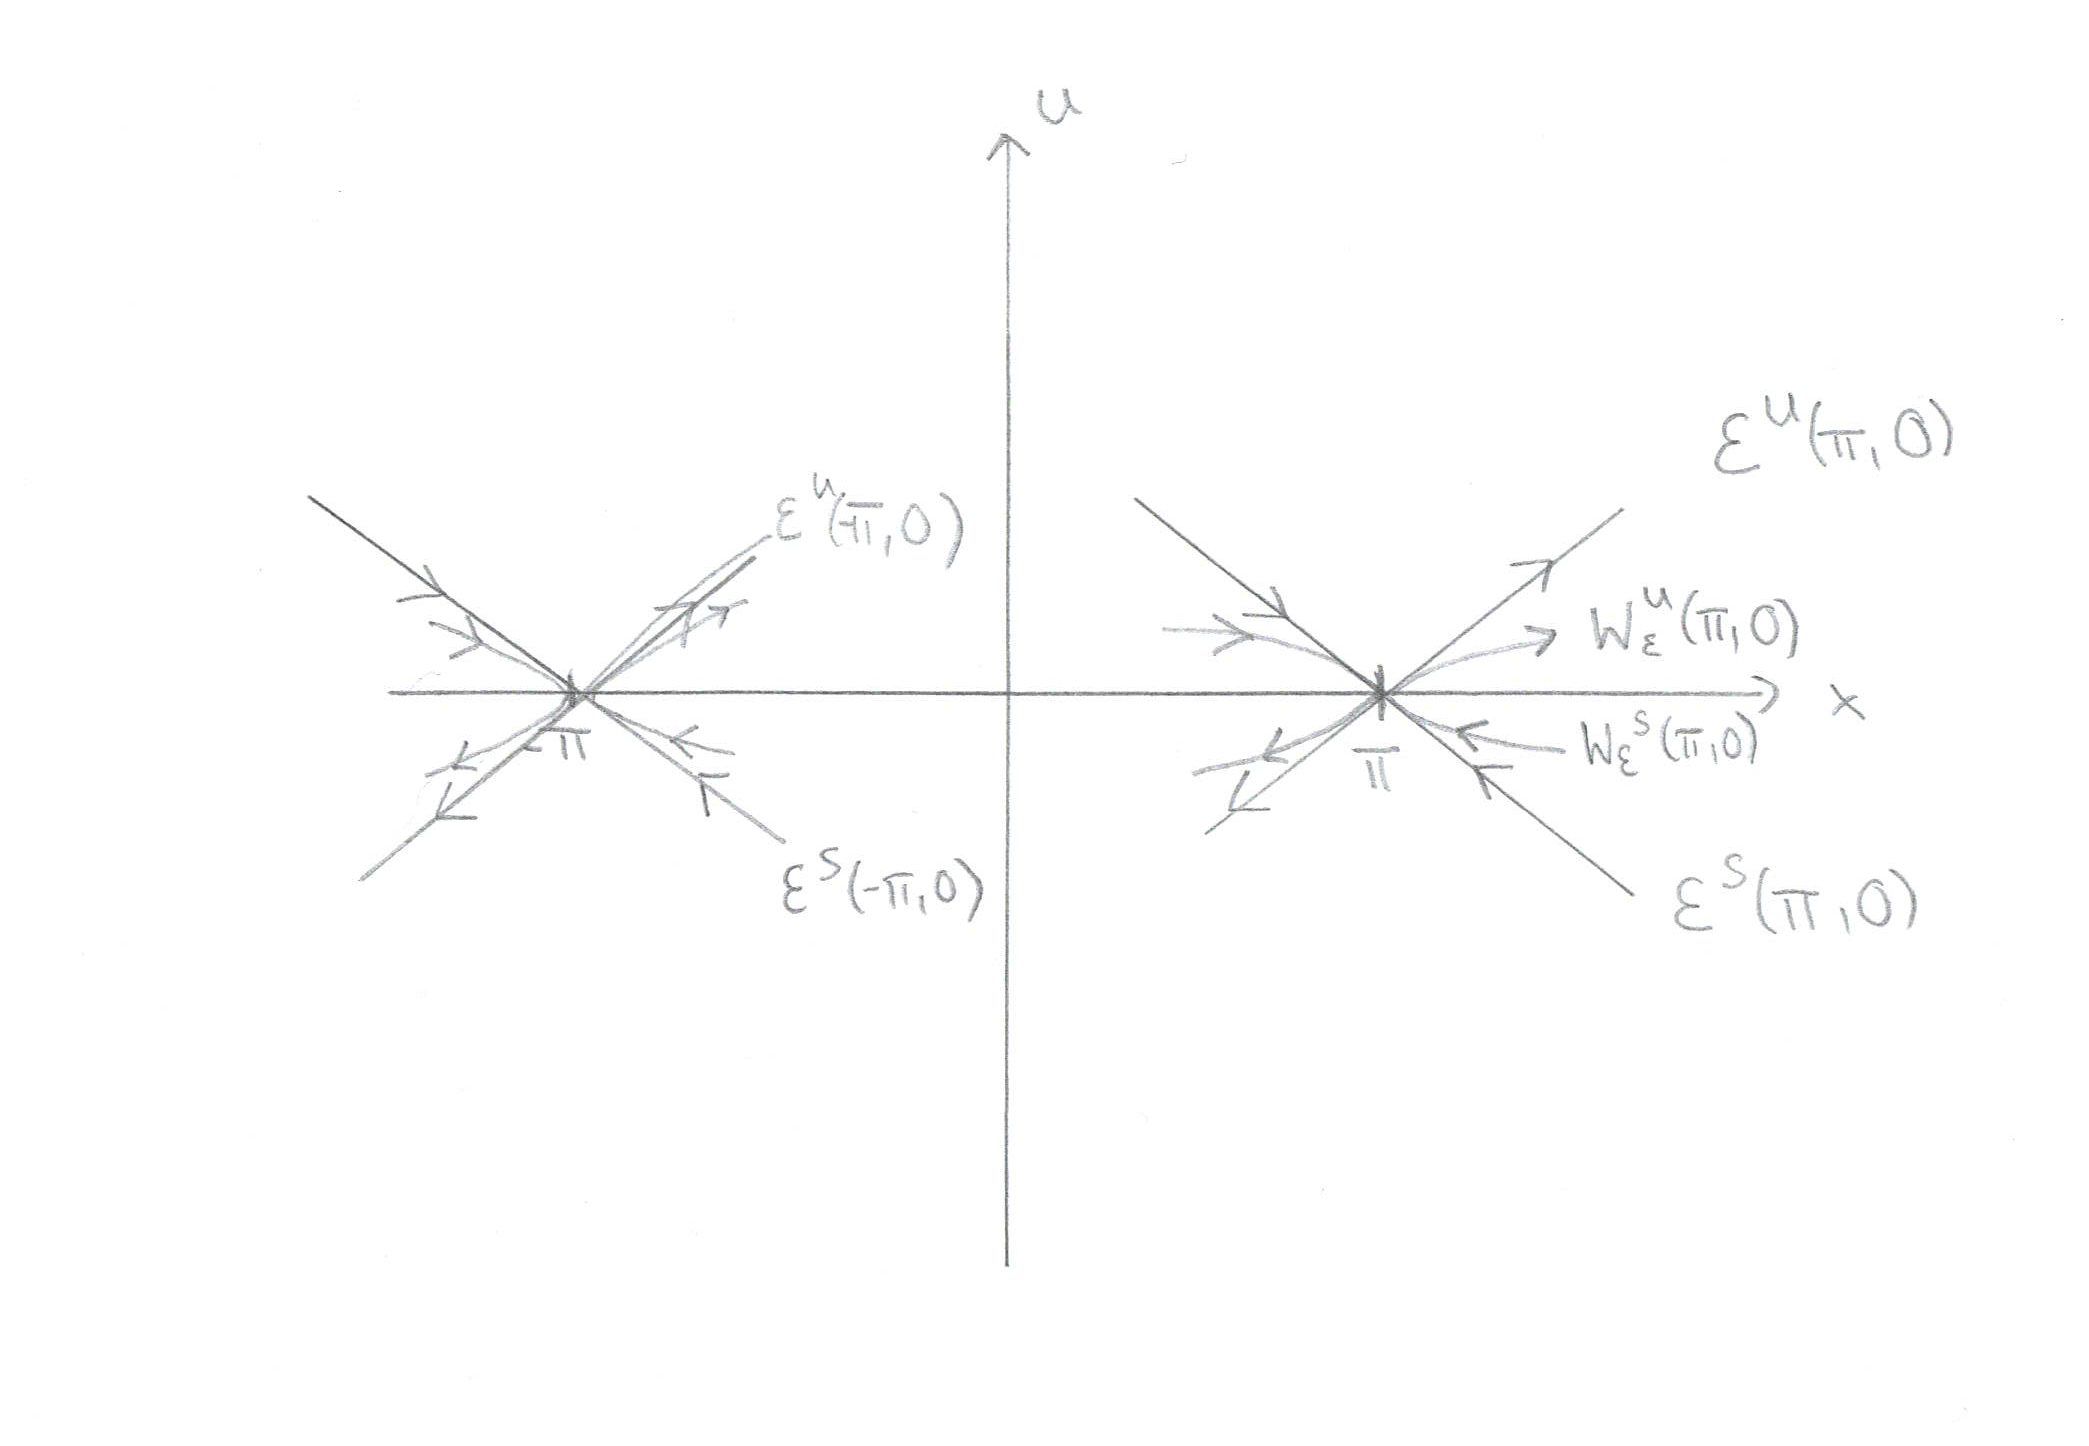
\includegraphics[width=12cm]{local_manifold.png}
\end{example}

\subsection{Gloabal invariant manifolds}
The global invariant manifolds are defined as
\begin{align*}
	W^s(\mathbf x_0) = \bigcup_{t \leq 0} \Phi^t(W_{\epsilon}^s(\mathbf x_0)) \quad \text{and} \quad
	W^u(\mathbf x_0) = \bigcup_{t \geq 0} \Phi^t(W_{\epsilon}^u(\mathbf x_0)).
\end{align*} 

\subsection{Discrete time}
The theory of absolutely parallel in the discrete time situation.
\begin{theorem}
	Consider a $\mathcal C^1$-map...
\end{theorem}
incomplete

\subsection{Center Subspaces}

\marginpar{\textbf{Week 08}\\Tue, 04.12}

\section{Bifurcations}

incomplete...

\marginpar{\textbf{Week 08}\\Thu, 06.12}

\section{Lagrangian Mechanics}

\subsection{Basic principles}
\begin{itemize}
	\item States point in the configuration space $X$. $X$ is a vector space in $\mathbb R^n$ or a manifold.
	
	\item The evolution of the mechanical system is a \textbf{curve} $\mathbf x: [t_0,t_1] \mapsto X, t \mapsto \mathbf x(t)$ in this space.
	
	\item Admissible curves\footnote{those which describe a real motion of the mechanical system} satisfy a minimisation  property. To formulate it, we need a function $\mathcal L({\mathbf x, \mathbf{\dot x}})$. If $X= \mathbb R^n$
	\[
		\mathcal L: \mathbb R^n \times \mathbb R^n \to \mathbb R 
	\]
	or if $X$ is a manifold
	\[
		\mathcal L: T_{\mathbf x}X \to \mathbb R.
	\]
	$\mathcal L$ is called the \textbf{Lagrange function}.
	
	\item The \textbf{action} along the curce $\mathbf{x}$ is defined as 
	\[
		S[\mathbf x] = \int^{t_1}_{t_0} \mathcal L(\mathbf x(t), \mathbf{\dot x(t)}) dt.
	\]
\end{itemize}

\subsection{Principle of least action}
\marginpar{\textbf{Week 09}\\Tue, 11.12}

The motion of a mechanical system with the Lagrange function $\mathcal L$ are those curves $\mathbf x: [t_0,t_1] \to X$ which deliver minimal critical points of the action functional $S[\mathbf x]$ under variations of the curve fixing its endpoints. 

Consider nearby curves $\mathbf y : [t_0, t_1] \to \mathbb R^n$ with $\mathbf y(t_0) = \mathbf x(t_0)$ and $\mathbf y(t_1)= \mathbf x(t_0)$. The variation of the curve is described by $\delta_{\mathbf x}: [t_0,t_1| \to \mathbb R^n, \delta_{\mathbf x} \coloneqq \mathbf y(t) - \mathbf x(t)$. For $\delta_{\mathbf x}(t_0)=\delta_{\mathbf x}(t_1) = 0$ the variation is null .

In the old classical formulation, the \textbf{principle of least action} is 
\[
	S[\mathbf x] \leq S[\mathbf x + \delta_{\mathbf x}]
\]
for all $\delta_{\mathbf x}$ which are sufficiently small.

\begin{example}
	Consider a natural mechanical system with the Lagrange function
	\[
		\mathcal L(\mathbf x, \mathbf{\dot x}) = K(\mathbf{\dot x}) - U(\mathbf x)
	\]	
	where $K$ is the kinetic energy and $U$ is the potential energy.
	
	\begin{itemize}
		\item Two body gravitational problem
		\begin{align*}
			K(\mathbf{\dot x}) = \frac{1}{2}m_1(\dot x_1^2+\dot y_1^2+\dot z_1^2) + \frac{1}{2}m_2(\dot x_2^2 + \dot y_2^2 + \dot z_2^2) \\
			U(\mathbf x) = - \frac{\gamma m_1m_2}{\sqrt{(x_1-x_2)^2 + (y_1-y_2)^2 + (z_1-z_2)^2}}
		\end{align*}
		
		\item Mathematical pendulum
		\begin{align*}
			K(\dot x) &= \frac{1}{2}m\dot x^2 \\
			U(x) &= -m\cdot g\cdot l\cdot \cos(x)
		\end{align*}
	\end{itemize}
\end{example}

Now, we will introduce some notations. We define the vector space $$\mathcal X = \mathcal X_{\mathbf x_0, \mathbf x_1} = \{ \mathbf x \in \mathcal C^1([t_0,t_1], \mathbb R^n) : \mathbf x(t_0) = \mathbf x_0, \mathbf(t_1) = \mathbf x_1 \}.$$
Note that $\mathcal X$ is \emph{not} a vector space but rather an affine space. The space of differences between elements in $\mathcal X$ is a vector space
\[
	\mathcal X_{\mathbf 0} = \mathcal X_{\mathbf 0, \mathbf 0}  = \{ \mathbf h \in \mathcal C^{1}([t_0,t_1], \mathbb R^n) : \mathbf h(t_0) = \mathbf 0, \mathbf h(t_1) = \mathbf 0 \}
\]
with norm $\Vert \mathbf h \Vert_1 = \sup\limits_{t \in [t_0,t_1]} (\Vert \mathbf h(t) \Vert + \Vert \mathbf{\dot h (t)} \Vert).$

\begin{definition}
	A functional $S: \mathcal X \to \mathbb R$ is called \textbf{differentiable} if for any curve $\mathbf x \in \mathcal X$ there exists a linear map $\delta S[\mathbf x] : \mathcal X_{\mathbf 0} \to \mathbb R$ such that
	\[
		S[\mathbf x + \mathbf h] - S[\mathbf x] = \delta S[\mathbf x]\mathbf h + o(\Vert \mathbf h \Vert_1), \quad \forall \mathbf h \in \mathcal X_{\mathbf 0}.
	\]
	
	We say that $\mathbf x \in \mathcal X$ delivers a \textbf{critical point} of $S$ if $\delta S[\mathbf x] = 0$. 
	
	We say that $\mathbf x \in \mathcal X$ delivers a \textbf{local minimum} of $S$ if $S[\mathbf x + \mathbf h] \geq S [\mathbf x]$ for all $h \in \mathcal X_{\mathbf 0}$ with $\Vert \mathbf h \Vert_1$ sufficiently small.
\end{definition}

\begin{theorem}
	The local minimum of a differentiable functional is its critical point.
\end{theorem}

\begin{theorem}
	If $\mathcal L: \mathbb R^n \times \mathbb R^n \to \mathbb R$ is $\mathcal C^2$, then the action functional $S[\mathbf x] = \int^{t_1}_{t_0} \mathcal L(\mathbf x(t), \mathbf{\dot x(t)}) dt$ is differentiable with
	\[
		\delta S[\mathbf x] h = \int^{t_1}_{t_0} \sum^n_{i=1} \underbrace{\left[
			\frac{\partial \mathcal L}{\partial x_i}\left(\mathbf x(t), \mathbf{\dot x}(t)\right) - \frac{d}{dt}\left( \frac{\partial \mathcal L}{\partial \dot x_i}(\mathbf x(t), \mathbf{\dot x}(t)) \right)
		\right]}_{\substack{\text{$\coloneqq E\mathcal L_i$ ... \textbf{Euler-Lagrange expression}} \\ \text{for the Lagrange function $\mathcal L$}}} h_i(t)dt.
	\]
\end{theorem}

\begin{proof}
	...
\end{proof}

\begin{theorem}
	A curve $\mathbf x \in \mathcal X$ is critical for the action $S$ if and only if it satisfies the \textbf{Euler-Lagrange differential equation}
	\[
		E\mathcal L_i = \frac{\partial\mathcal L}{\partial x_i} - \frac{d}{dt}\left( \frac{\partial \mathcal L}{\partial \dot x_i} \right) = 0, \quad \text{for all }i = 1,...,n.
	\]
\end{theorem}

In order to prove this theore we will need the following lemma.

\begin{lemma}
	Let $f: [t_0,t:1] \to \mathbb R$ be continuous. If for all...
\end{lemma}

\begin{proof}[Proof of Lemma.]
	Inhalt...
\end{proof}

\begin{proof}[Proof of Theorem.]
	The lemma proves the theorem for $n=1$. To prove it for $n > 1$ use the lemma componentwise.
\end{proof}

\begin{example}
	The Euler-Lagrange equations for natural mechanical systems are given by 
	\begin{align*}
		\mathcal L(\mathbf x, \mathbf{\dot x}) &= \frac{1}{2} \langle \mathbf{\dot x}, M \mathbf{\dot x} \rangle - U(\mathbf x), \quad M \in \mathrm{Symm}(n) \\
		&= \frac{1}{2}\sum^n_{i,j=1}m_{ij}\dot x_i\dot x_j - U(x_1,...,x_n)
	\end{align*}
	The Euler-Lagrange expression is 
	\[
		E\mathcal L_i = \frac{\partial \mathcal L}{\partial x_i} - \frac{d}{dt}\left( \frac{\partial \mathcal L}{\partial \dot x_i} \right) = -\frac{\partial U}{\partial x_i} - \frac{d}{dt} \sum^n_{j=1} m_{ij}\dot x_j = -\frac{\partial U}{\partial x_i} - \sum^n_{j=1} m_{ij}\ddot x_j.
	\]
	So the Euler-Lagrange differential equation $E\mathcal L_i = 0$ yields
	\begin{framed}
	\[
		\sum^n_{j=1} m_{ij} \ddot x_j = -\frac{\partial U}{\partial x_i}, \quad i = 1,...,n.
	\]
	\end{framed}
	Those are implicit second order differential equations
	\begin{framed}
	\[
		M \mathbf{\ddot x} = - \Delta U.
	\]
	\end{framed}
\end{example}

Usually, one would like to the Euler Lagrange equations for $\ddot x_i = g_i(\mathbf x, \mathbf{\dot x})$. For natural mechnical system, one needs $\det M \neq 0$ for this so that
\[
\mathbf{\ddot x} = \underbrace{-M^{-1}\Delta U(\mathbf x)}_{=g(\mathbf x)}.
\]
In general
\[
	E\mathcal L_i = \frac{\partial \mathcal L}{\partial x_i} - \frac{d}{dt}\left( \frac{\partial \mathcal L}{\partial \dot x_i} \right) = \frac{\partial \mathcal L}{\partial x_i} - \underbrace{\sum^n_{j=1}\frac{\partial^2 \mathcal L}{\partial \dot x_i \partial x_j}\dot x_j}_{\text{complicated}} - \underbrace{\sum^n_{j=1} \frac{\partial^2 \mathcal L}{\partial \dot x_i \partial \dot x_j}\ddot x_j}_{\text{easy}}.
\]
To solve the system of Euler Lagrange equations for $\ddot x_j = g_j(\mathbf x, \mathbf{\dot x})$ one needs the \textbf{non-degeneracy condition} $$\det(\frac{\partial^2 \mathcal L}{\partial \dot x_i \partial \dot x_j})_{i,j=1,...,n} \neq 0.$$

\begin{theorem}
	Euler Lagrange equations admit a conserved quantity
	\[
		E(\mathbf x, \mathbf{\dot x}) = \sum^n_{i=1}\dot x_i \frac{\partial \mathcal L}{\partial \dot x_i} - \mathcal L(\mathbf x, \mathbf{\dot x}).
	\]
\end{theorem}

\begin{proof}
	dwdw
\end{proof}

\begin{example}
	For natural mechanical systems
	\[
		E(\mathbf x, \mathbf{\dot x}) = \sum^n_{i=1}
	\]
\end{example}

\marginpar{\textbf{Week 09}\\Thu, 13.12}

\subsection{Submanifolds in $\mathbb R^n$}

We will give a quick introduction into submanifolds in $\mathbb R^n$ before we move to Lagrangian mechanics on manifolds.

\begin{definition}
	$M \subset \mathbb R^n$ is called a $d$-dimensional differentiable submanifold in $\mathbb R^n$ if any point $\mathbf p \in M$ has an open neighbourhood $U \subset \mathbb R^n$ and a diffeomorphism\footnote{$H$ is a diffeomorphism if it is bijective and differentiable, and its inverse is differentiable.} $H: U \to U'$ onto an open neighbourhood $U' \subset \mathbb R^n$ such that 
	\[
		H(M \cap U) = (\mathbb R^d \times \mathbf 0^{n- d}) \cap U'.
	\]
\end{definition}

In any neighbourhood of $\mathbf p \in M$ the manifold $M$ looks like a small piece of $\mathbb R^d$.

\subsection{Lagrangian mechanics on manifolds under holonomic constraints}

There are two kinds of constraints
\begin{itemize}
	\item holonomic $f_i(\mathbf x) = \mathbf 0$ for $i = 1,...,n$. This is the case which we will treat in our course.
	\item non-holonomic $f_i (\mathbf x, \mathbf{\dot x}) = \mathbf 0 $. We won't discuss this.
\end{itemize}

 Let $M$ be the configuration manifold and $\mathcal L: TM \to \mathbb R$. For any curve $\mathbf x:[t_0,t_1] \to M$ the action along $\mathbf x$ is given by $$S[\mathbf x] = \int_{t_0}^{t_1}\mathcal L(\mathbf x(t), \underbrace{\mathbf{\dot x}(t))}_{\in T_{\mathbf x(t)}} dt.$$ 
 Motions of a mechanical systems are critical points of the action $S$, i.e. curves $\mathbf x$ with fixed endpoints  at $\mathbf x(t_0) = \mathbf x_0$ and $\mathbf x(t_1) = \mathbf x_1$ and which are stationary values of the action $S$ (least action principle). We are interested in finding stationary values of $S$ since these are the admissable curves of the system. The remarkable insight is (due to Euler and Lagrange) that there is a single method which deals with all kinds of questions concerning the analysis of stationary values of an functional of the form
 \[
 	I[y] = \int^b_a F(y, \dot y) dt
 \]
 for general $F$. This approach has many applications in physics due to the fact that the concept of stationary values is independent of coordinates.
 
 The idea of finding stationary values is rooted in the idea that small variations $\mathbf x(t) + \epsilon \mathbf v(t)$ of a curve $\mathbf x(t)$ are close to the tangent space $T_{\mathbf x(t)}M$. Infinitesimal variations of $\mathbf x(t)$ are given by $\mathbf x(t) + \epsilon \mathbf{v}(t)$ where $\mathbf v: [t_0,t_1] \to TM$ with $\mathbf v(t) \in T_{\mathbf x(t)}M$ and $\mathbf v(t_0) = \mathbf 0 = \mathbf v(t_1)$. 

\[
	\delta S[\mathbf x] \mathbf v  = 0 \iff \frac{d}{d\epsilon}S[\mathbf x + \epsilon \mathbf v] \Big |_{\epsilon = 0} = 0.
\]



\marginpar{\textbf{Week 10}\\Tue, 18.12}

\begin{example}
	The mathematical pendulum is described by
	\[
		\mathcal L(\mathbf x, \mathbf y, \mathbf{\dot x}, \mathbf{\dot y}) = \frac{1}{2}m(\mathbf{\dot x}^2 + \mathbf{\dot y}^2) - mg\mathbf y.
	\]
\end{example}

\marginpar{\textbf{Week 10}\\Thu, 20.12}

\subsection{Noether's theorem}

We do not prove the full version. Nevertheless, everything is based on integration by parts (as usual in variatoinal calculus).

\section{Hamiltonian mechanics}
\subsection{Basic principles}
In textbooks the Hamiltonian mechanics is described as the more fundamental formulation of classical mechanics in comparison to the Lagrangian Mechanics. To obtain a Hamiltonian system, we transform the Lagrangian systen with Lagrange function $\mathcal L$ by a Legrende transformation. Given a point $(\mathbf x, \mathbf{\dot x})$ in the configuration space, we introduce a new variable $\mathbf p \in \mathbb R^n$, that we call \textbf{conjugate momentum}. The momentum is defined as
\[
	\mathbf p = \frac{\partial L}{\partial \mathbf{\dot x}}(\mathbf x, \mathbf{\dot x})
\]
and in components for $i = 1,...,n$
\[
	\mathbf p_i = \frac{\partial \mathcal L}{\partial\mathbf{\dot x_i}}(\mathbf x, \mathbf{\dot x}).
\]
The conjugate momentum $\mathbf p \in T_{\mathbf x}^*X$ is a \textbf{covector}, and $ T_{\mathbf x}^*X$ is called the \textbf{cotangent space} at $\mathbf x$. The cotangent space is the dual space of $T_\mathbf{x}X$, i.e. every $a \in T_{\mathbf x}^*X$ is linear functional with $a: T_{\mathbf x}X \to \mathbb R$. So, $\mathbf p$ is linear functional that takes points in the configuration space $T_xX$, and maps them to the derivative of $\mathcal L$ with respect to the velocity $\mathbf{\dot x}$.

If we have a Lagrangian system, we use the \textbf{Legrende transformation}
\[
	(\mathbf x, \mathbf{\dot x}) \mapsto (\mathbf x, \mathbf p) = (\mathbf x, \frac{\partial L}{\partial \mathbf{\dot x}}(\mathbf x, \mathbf{\dot x}))
\]
to obtain the Hamiltonian system. The configuration space which was previously in $TX$ is now in $T^*X$. The second component is not the velocity $\mathbf{\dot x} \in T_{\mathbf x}X$ but the conjugate momentum $\mathbf p \in T_{\mathbf x}^*X$. We will later see why this transformation is useful for physical applications.

There is just one problem: the transformation may not be invertible. Thus, we do only consider systems where the Legrende transformation $(\mathbf x, \mathbf{\dot x}) \mapsto \mathbf p$ is invertible, i.e. we can reconstruct the velocity given the position $\mathbf x$ and the conjugate momentum $\mathbf p$ by
\[
	\mathbf{\dot x} = \mathbf{\dot x(\mathbf x, \mathbf p)}.
\]
We also provide a condition when the Legrende transformation is non-degenerate: the determinant of the Hessian matrix of $\mathcal L$ with respect to $\mathbf{\dot x}$ must be non-zero\footnote{Note that the same non-degeneracy condition was used to ensure that the Euler-Lagrange equations are $2$nd order differential equations and invariant under changes of coordinates.}
\[
	\left| \left( \frac{\partial^2 \mathcal L}{\partial \dot x_i \partial \dot x_j}\right)_{i,j=1}^n  \right| \neq 0.
\]
We introduce the \textbf{Hamilton function}, which will replace the Lagrange function in Hamiltonian systems. We start by defining the Hamilton function $H$ as the total energy function, where the velocity depends on the conjugate momentum
\begin{align*}
	H(\mathbf x, \mathbf p) &= E(\mathbf x, \mathbf{\dot x})\Big \vert_{\mathbf{\dot{x}} = \mathbf{\dot x(\mathbf x, \mathbf p)}}\\
	&= \left(\sum^n_{k=1} \dot x_k \frac{\partial \mathcal L}{\partial \dot x_k} - \mathcal L(\mathbf x, \mathbf{\dot x})\right) \Big |_{\mathbf{\dot x} = \mathbf{\dot x}(\mathbf x, \mathbf p)}.
\end{align*}
Using the identity $\mathbf p = \frac{\partial \mathcal L}{\partial\mathbf{\dot x}}$, we obtain
\begin{framed}
	The Legrende transformation of $\mathcal L(\mathbf x, \mathbf{\dot x})$ is given by
	\[
		H(\mathbf x, \mathbf p) = \left(\sum^n_{k=1} \dot x_k p_k - \mathcal L(\mathbf x, \mathbf{\dot x}) \right)
		 \Big |_{\mathbf{\dot x} = \mathbf{\dot x}(\mathbf x, \mathbf p)} = \Big( \langle \mathbf x, \mathbf p \rangle - \mathcal L(\mathbf{ x}, \mathbf{\dot x}) \Big)
		 \Big |_{\mathbf{\dot x} = \mathbf{\dot x}(\mathbf x, \mathbf p)}
	\]
\end{framed}
The Hamilton function maps from $T^*X$ to $\mathbb R$. In comparision, the Lagrange function maps from $TX$ to $\mathbb R$. Interestingly, the partial derivatives of $H$ are easy to compute:
\begin{align*}
\frac{\partial H}{\partial p_j} = \dot x_j + \sum^n_{k=1} \frac{\dot x_k}{\partial p_j}p_k - \sum^n_{k=1} \underbrace{\frac{\partial \mathcal L}{\partial \dot x_k}}_{=p_k} \frac{\partial \dot x_k}{\partial p_j} = \dot x_j
\end{align*}
and
\begin{align*}
\frac{\partial H}{\partial x_j} &= \sum^n_{k=1} \frac{\partial \dot x_k}{\partial x_j}p_k - \frac{\mathcal L}{\partial x_j}(\mathbf x, \mathbf{\dot x}(\mathbf x, \mathbf p))\\
&\Downarrow \text{By chain rule: $\frac{\partial u(v(t),w(t))}{\partial t} = \frac{\partial u}{\partial v} \frac{\partial v}{\partial t} + \frac{\partial u}{\partial w}\frac{\partial w}{\partial t}$}\\
 &= \sum^n_{k=1} \frac{\partial \dot x_k}{\partial x_j}p_k - \frac{\partial \mathcal L}{\partial x_j} - \sum^n_{k=1} \underbrace{\frac{\partial \mathcal L}{\partial \dot x_k}}_{=p_k} \frac{\partial \dot x_k}{\partial x_j}  \\
 &= - \frac{\partial \mathcal L}{\partial x_j} \\
 &\Downarrow \text{Euler-Lagrange equations}\\
 &= - \frac{d}{dt}\left( \frac{\partial \mathcal L}{\partial \dot x_j}\right)\\
 &= - \frac{d}{dt}p_j\\
 &= - \dot p_j.
\end{align*}

Using the coordinates $\mathbf x$ and $\mathbf p$, the motions of the system are given by \textbf{Hamilton's equations of motions}
\begin{framed}
	\[
		\dot x_j = \frac{\partial H}{\partial p_j} \quad \text{and} \quad \dot p_j = -\frac{\partial H}{\partial x_j} \quad j = 1,...,n.
	\]
\end{framed}

This is good news for we get a system of $2n$ first order ordinary differential equations. Before, we had a system of second order differential equations in the form of Euler-Lagrange equations. We increase the dimensions, but as a tradeoff we obtain a first order system of ODEs. This allows us to directly solve the linear system of differential equations; no more variational principles or least action principles are needed to obtain solutions!

Generally, we consider Hamiltonian systems opearting on $H: T^*X \to \mathbb R$ or $H: \mathbb R^{2n} \to \mathbb R$. Hence, Hamilton functions take vectors of dimension $2n$ with $(x_1,...,x_n,p_1,...,p_n)$. The dimension of the configuration space - also known as \emph{degree of freedom} - is $n$. The system is called $n$ degree-of-freedom Hamiltonian system. The configuration space $T^*X$ and $\mathbb R^{2n}$ are called the \emph{canonical phase space} of dimension $2n$.

Note that the system of linear differential equations is autonomous, i.e. independent of $t$. Thus, everything we have learned so far about dynamical systems is applicable in our theory. Let us examine some examples.

\begin{example}
Consider a natural mechanical system with Lagrange function
\[
	\mathcal L(\mathbf x, \mathbf{\dot x}) = \frac{1}{2}\langle \mathbf{\dot x}, M \mathbf{\dot x} \rangle - U(\mathbf x).
\]
The Legrende transformation of the Lagrangian system is given by
\[
	\mathbf p = M \mathbf{\dot x} 
\]
and the inverse of the transformation is
\[
	\mathbf{\dot x} = M^{-1}\mathbf p.
\]
Thus, the Hamilton function reads
\begin{align*}
H(\mathbf x, \mathbf p) &= \left(\langle \mathbf{\dot x}, \mathbf p \rangle - \mathcal L(\mathbf x, \mathbf{\dot x}) \right) \Big |_{\mathbf{\dot x} = M^{-1}\mathbf p} \\
&= \langle M^{-1}\mathbf p, \mathbf p \rangle - \frac{1}{2}\langle \mathbf{\dot x}, M \mathbf{\dot x} \rangle \Big |_{\mathbf{\dot x}= M^{-1}\mathbf p} + U(\mathbf x) \\
&= \langle M^{-1}\mathbf p, \mathbf p \rangle - \frac{1}{2}\langle M^{-1} \mathbf p, \mathbf p \rangle + U(\mathbf x) \\
&= \underbrace{\frac{1}{2} \langle M^{-1}\mathbf p, \mathbf p \rangle}_{\text{kinetic energy}}  + \underbrace{U(\mathbf x)}_{\text{potential energy}}.
\end{align*}
Thus, the Hamilton function of a natural mechanical system is the total energy function. As we will later see, the Hamilton function is always an integral of motion of the Hamiltonian system!
\end{example}

The \textbf{Hamiltonian vector field} $X_H$ of the Hamiltonian system
\[
	\begin{cases}
	\dot x_k = \frac{\partial H}{\partial p_k} \\
	\dot p_k = -\frac{\partial H}{\partial x_k}
	\end{cases}
\]
is given by
\[
	X_H = \begin{pmatrix}
		(\frac{\partial H }{\partial p_k})^n_{k=1} \\ -(\frac{\partial H}{\partial x_k})^n_{k=1}
	\end{pmatrix} = \begin{pmatrix}
	 \grad_{\mathbf p}{H} \\
	 -\grad_{\mathbf x}{H}
	\end{pmatrix}.
\]
Thus, we can write the Hamiltonian system as 
\[
	(\mathbf{\dot x}, \mathbf{\dot p}) = X_H(\mathbf x, \mathbf p).
\]

\textit{A good overview of Hamiltonian mechanics can be found on \url{http://www.scholarpedia.org/article/Hamiltonian_systems}.}

\subsection{General properties of Hamiltonian systems}
\begin{itemize}
	\item $H(\mathbf x,\mathbf p)$ is an integral of motion for the system
	\[
		\begin{cases}
			\dot x_k = \frac{\partial H}{\partial p_k} \\
			\dot p_k = -\frac{\partial H}{\partial x_k}
		\end{cases} 
	\]
	\begin{proof}
		To see this, we compute the Lie-derivative of the Hamilton function $H$ under the vector field $X_H$, i.e. 
		\begin{align*}
			\mathcal L_{X_H}H = \sum^n_{k=1}\left( 
				\frac{\partial H}{\partial x_k}\dot x_k + \frac{\partial H}{\partial p_k}\dot p_k
			\right) = 
			\sum^n_{k=1} \left( 
				\frac{\partial H}{\partial x_k} \frac{\partial H}{\partial p_k} + \frac{\partial H}{\partial p_k}(- \frac{\partial H}{\partial x_k}) = 0.
			\right)
		\end{align*}
	\end{proof}

\marginpar{\textbf{Week 11}\\Tue, 08.01}
	\item asdasd
\end{itemize}

\subsection{Poisson bracket}

\subsection{Quick introduction: Alternating forms and differential forms}



not quite complete, one example missing 

\marginpar{\textbf{Week 12}\\Tue, 15.01}

\begin{theorem}
	If a flow of a vector field $X$ on $\mathbb R^{2n}(x,p)$ preserves the canonical two form $\omega = \sum^n_{k=1} dx_k \land dp_k$, then (locally) there exists $H: \mathbb R^{2n} \to \mathbb R$ such that $X = X_H = \begin{pmatrix}
	\mathrm{grad}_pH \\ \mathrm{-grad}_xH
	\end{pmatrix} = \begin{pmatrix}
	0 & I \\ -I & 0
	\end{pmatrix} \mathrm{grad} H$.
\end{theorem}

\begin{proof}
	Let 
	\[
	X = \begin{pmatrix}
	f_1(x,p) \\ \vdots \\ f_n(x,p) \\ g_1(x,p) \\ g_n(x,p)
	\end{pmatrix}
	\]
	so that $\begin{cases}
	\dot x_k = f_k(x,p) \\ \dot p_k ) g_k(x,p)
	\end{cases}$. 
	Assume that
	\begin{align*}
	L_x\omega = 0 &\iff \sum_{k=1}^n (df_k(x,p) \land dp_k + dx_k \land dg_k(x,p)) = 0\\
	&\iff \sum^n_{k=1}(\sum^n_{j=1} (\frac{\partial f_k}{\partial x_j} dx_j + \frac{\partial f_k}{\partial p_j} dp_j) \land dp_k + dx_k \land 
	(\sum_{j=1}^n \frac{\partial g_k}{\partial x_j} dx_j + \frac{\partial g_k}{\partial p_j}\land dp_j) ) = 0.
	\end{align*}
	Coefficients by $dx_k \land dx_j ; \frac{\partial g_k}{\partial x_j} - \frac{\partial g_j}{\partial x_k} = 0$. By $dp_j \land dp_k: \frac{\partial f_k}{\partial p_j} - \frac{\partial f_j}{\partial p_k} = 0$. By $dx_j \land dp_k: \frac{\partial f_k}{\partial x_j} - \frac{\partial g_j}{\partial p_k} = 0$. The first condition is that there exists a function $H_1$ (defined up to a function of $p$) such that locally it holds $g_k = \frac{\partial H_1}{\partial x_k}$. The second condition is that there exists a function $H_2$ (defined up to a function of $x$) such that locally it holds $f_k = \frac{\partial H_2}{\partial p_k}$. Additionally 
	\begin{align*}
	\frac{\partial}{\partial x_j} (\frac{\partial H_2}{\partial p_k}) + \frac{\partial }{\partial p_k} (\frac{\partial H_1}{\partial x_j}) = 0 &\iff \frac{\partial^2}{\partial x_j \partial p_k} (H_1 + H_") = 0 \\
	&\iff H_1(x,p) + H_2(x,p) = a(x) + b(p) \\
	& \iff H_1(x,p) - b(p ) = -H_"(x,p) + a(x) \coloneqq -H(x,p).
	\end{align*} 
	Then $f_k = \frac{\partial H}{\partial p_k} , g_k = -\frac{\partial H}{\partial x_k}$.
\end{proof}

An example of a locally Hamiltonian vector field which is not globally Hamiltonian. Consider a vector field on a non-simply-connected manifold - a torus[1]. A torus is analytically described by $(\mathbb R \setminus \mathbb Z)^2 = S^1 \times S^1 = \{ (x(\mod 1), p(\mod 1))  \}$. The canonical two form of the torus is 
\[
\omega = dx \wedge dp \quad \text{it measures the area of the torus.}
\]
The simples vector field is $\begin{cases}
\dot x =1 \\ \dot p = 0
\end{cases}$. It just describes a translation. We claim that this vector field is locally Hamiltonian $\begin{pmatrix}
\frac{\partial H}{\partial p} = 1 \\ \frac{\partial H}{\partial x} = 0
\end{pmatrix}$, but $H(x,p) = p$ is not a smooth function on the torus since it gets an increment $\neq 0$ along closed non-null-homotopic curves $x = \mathrm{const}$.

\begin{definition}
	A map $\varphi: \mathbb R^{2n}_{(x,p)} \to \mathbb R^{2n}_{(x,p)}$ preserving $\omega = \sum^n_{k=1} dx_k \wedge dp_k$ (that is $\varphi^* \omega = \omega$) is called a \textbf{symplectic map} (so that the flow of $X_H$ consists of symplectic maps).
\end{definition}

\begin{definition}
	A matrix $D \in \mathrm{mat}_{2n \times 2n} (\mathbb R)$ is symplectic, i.e. $D \in \mathrm{Sp}_{2n}(\mathbb R)$, if it satisfies 
	\[
	D^TJD = J \quad \text{ with $J = \begin{pmatrix}
		0 & I \\ -I & 0
		\end{pmatrix}$}.
	\]
	
\end{definition}

\begin{theorem}
	A map $\varphi$ is symplectic if and only if $d \varphi \in \mathrm{mat}_{2n \times 2n}(\mathbb R)$ is symplectic.
\end{theorem}

\begin{proof}
	Let $(\tilde x, \tilde p) = \varphi(x,p)$. 
	\begin{align*}
	\sum^n_{k=1} d\tilde x_k \wedge d\tilde p_k =\sum^n_{k=1}
	\sum^n_{j=1}(\frac{\partial \tilde x_k}{\partial x_j} dx_j + \frac{\partial \tilde  x_k}{\partial p_j} dp_j) \wedge \sum^n_{i=1}(\frac{\partial \tilde p_k}{\partial x_i} dx_i + \frac{\partial \tilde p_k}{\partial p_i} dp_i) \\
	\sum^n_{j=1} \sum^n_{i=1} (\sum^n_{k=1} \frac{\partial \tilde x_k}{\partial x_j} \frac{\partial \tilde p_k}{\partial x_i} dx_j \wedge dx_i)  + 
	\sum^n_{j=1} \sum^n_{i=1} (\sum^n_{k=1} \frac{\partial \tilde x_k}{\partial p_j} \frac{\partial \tilde p_k}{\partial p_i} dp_j \wedge dp_i) +
	\sum^n_{j=1} \sum^n_{i=1} (\frac{\partial \tilde x_k}{\partial x_j} \frac{\partial \tilde p_k}{\partial p_i} - \frac{\partial \tilde x_k}{\partial p_i} \frac{\partial \tilde p_k}{\partial x_j}) dx_j \wedge dx_i\\
	\end{align*} 
	This should be equal to $\sum^n_{j=1} dx_j \wedge dp_j$.
	
	Coefficients by $dx_j \wedge dx_i: \sum^n_{k=1} \frac{\partial \tilde x_k}{\partial x_j} \frac{\partial \tilde p_k}{\partial x_i}  - \frac{\partial \tilde x_k}{\partial x_i} \frac{\partial \tilde p_j}{ \partial x_k} = 0 \iff (\frac{\partial \tilde x}{\partial x})^T \frac{\partial \tilde p}{\partial x} - (\frac{\partial \tilde p}{\partial x})^T(\frac{\partial \tilde x}{\partial x}) = 0_{n \times n}$.
	
	Coefficients by $dp_j \wedge dp_i: \sum^n_{k=1} \frac{\partial \tilde x_k}{\partial p_j} \frac{\partial \tilde p_k}{\partial p_i}  - \frac{\partial \tilde x_k}{\partial p_i} \frac{\partial \tilde p_k}{ \partial p_j} = 0 \iff (\frac{\partial \tilde x}{\partial p})^T \frac{\partial \tilde p}{\partial p} - (\frac{\partial \tilde p}{\partial p})^T(\frac{\partial \tilde x}{\partial p}) = 0_{n \times n}$. 
	
	Coefficients by $dx_j \wedge dp_i: \sum^n_{k=1} \frac{\partial \tilde x_k}{\partial x_j} \frac{\partial \tilde p_k}{\partial p_i}  - \frac{\partial \tilde x_k}{\partial p_i} \frac{\partial \tilde p_k}{ \partial x_j} = \delta_{ij} \iff 
	(\frac{\partial \tilde x}{\partial x})^T \frac{\partial \tilde p}{\partial p} - (\frac{\partial \tilde p}{\partial x})^T \frac{\partial \tilde x}{\partial p} = I_{n \times n}
	$
	
	This is is equivalent to
	\[
	\begin{pmatrix}
	\frac{\partial \tilde x}{\partial x} & \frac{\partial \tilde x}{\partial p} \\
	\frac{\partial \tilde p}{\partial x} & \frac{\partial \tilde p}{\partial p}
	\end{pmatrix}^T \begin{pmatrix}
	0 & I \\ -I & 0
	\end{pmatrix} \begin{pmatrix}
	\frac{\partial \tilde x}{\partial x} & \frac{\partial \tilde x}{\partial p} \\
	\frac{\partial \tilde p}{\partial x} & \frac{\partial \tilde p}{\partial p}
	\end{pmatrix} = \begin{pmatrix}
	0 & I \\ -I & 0
	\end{pmatrix}.
	\]
\end{proof}
\begin{definition}
	$Sp_{2n} \coloneqq \{ D \in mat_{2n \times 2n} (\mathbb R): D^TJD = J \}$ is called the symplectic group.
\end{definition}

Based on 
\begin{itemize}
	\item $D_1^TJD_1 = J, D_2^TJD_2 = J \implies (D_1D_2)^T J (D_1D_2) = J$ 
	\item $\det D \neq 0: \det(D^TJD) = \det(D)\det(J)\det(D) = \det(J) \implies (\det(D))^2 = 1 \implies \det(D) = \pm1$.
	\item $D^TJD = J \iff (D^{-1})^TJ(D^{-1}) = J$.
\end{itemize} 
Thus, $\mathrm{Sp}_{2n}(\mathbb R)$ is a group, indeed.

Some side remarks: Classical matrix Lie groups
\begin{gather*}
\mathrm{GL}_n(\mathbb R) = \{ A \in \mathrm{mat}_{n \times n}(\mathbb R) : \det(A) \neq 0 \} \\
O_n(\mathbb R) = \{ A \in \mathrm{mat}_{n \times n}(\mathbb R): A^T A = I \} \\
\mathrm{Sp}_{2n}(\mathbb R) = \{ A \in \mathrm{mat}_{2n \times 2n}(\mathbb R): A^TJA = J \}
\end{gather*}
The group $\mathrm{Sp}_{2n}(\mathbb R)$ preserves skew symmetric two forms.

We know for othrogonal matrices if the row form an orthonormal basis so do the columns, i.e. $A^T A = I$ and $AA^T = I$. Something similar also holds for the symplectic matrices.

\begin{theorem}
	It holds: $D \in \mathrm{Sp}_{2n}(\mathbb R) \iff DJD^T = J$.
\end{theorem}

\begin{proof}
	\begin{align*}
	D^TJD = J \iff JD = (D^T)^{-1}J \overset{J^{-1} = -J}{\iff} D = -J(D^T)^{-1}J &\iff DJ = J(D^T)^{-1} \\ &\iff DJD^T = J.
	\end{align*}
\end{proof}

\begin{collorary}
	Symplectic maps preserve Poisson brackets.
\end{collorary}
\begin{proof}
	For $D = d\varphi = \begin{pmatrix}
	\frac{\partial \tilde x}{\partial x} & \frac{\partial \tilde x}{\partial p} \\
	\frac{\partial \tilde p}{\partial x} & \frac{\partial \tilde p}{\partial p}
	\end{pmatrix}$ the identitiy $DJD^T = J$ reads
	\begin{align*}
	\frac{\partial \tilde x}{\partial x}(\frac{\partial \tilde x}{\partial p})^T - \frac{\partial \tilde x}{\partial p}(\frac{\partial \tilde x}{\partial x})^T = 0
	\iff \sum^n_{k=1}(\frac{\partial \tilde x_i}{\partial x_k} \frac{\partial \tilde x_j}{\partial p_k} - \frac{\partial \tilde x_i}{\partial p_k} \frac{\partial \tilde x_j}{\partial x_k}) = 0
	\\
	\frac{\partial \tilde p}{\partial p}(\frac{\partial \tilde x}{\partial p})^T - \frac{\partial \tilde p}{\partial p}(\frac{\partial \tilde x}{\partial x})^T = 0 
	\iff \sum^n_{k=1}(\frac{\partial \tilde p_i}{\partial x_k} \frac{\partial \tilde p_j}{\partial p_k} - \frac{\partial \tilde p_i}{\partial p_k} \frac{\partial \tilde p_j}{\partial x_k}) = 0
	\\
	\frac{\partial \tilde x}{\partial x}(\frac{\partial \tilde p}{\partial p})^T - \frac{\partial \tilde x}{\partial p}(\frac{\partial \tilde p}{\partial x})^T =  I 
	\iff \sum^n_{k=1}(\frac{\partial \tilde x_i}{\partial x_k} \frac{\partial \tilde p_j}{\partial p_k} - \frac{\partial \tilde x_i}{\partial p_k} \frac{\partial \tilde p_j}{\partial x_k}) = \delta_{i,j}.
	\end{align*}
	This is equivalent to $\{ \tilde x_i \tilde x_j \} = 0 = \{ x_i,x_j \}, \{ \tilde p_i \tilde p_j \} = 0 = \{ p_i,p_j \}, \{ \tilde x_i \tilde p_j \} = \delta_{i,j} = \{ x_i,p_j \}$.
\end{proof}

This means that the map $\varphi: \mathbb R^{2n} \to \mathbb R^{2n}$ is a \textbf{Poisson map}. 
\begin{definition}
	A map $\varphi: \mathbb R^{2n} \to \mathbb R^{2n}$ is called a \textbf{Poisson map} if it preserves the Poisson brackets: in coordinates, 
	\begin{align*}
	\{\tilde x_i, \tilde  x_j \} = \{ x_i,x_j \} = 0 \\
	\{\tilde p_i, \tilde  p_j \} = \{ p_i,p_j \} = 0 \\
	\{\tilde x_i, \tilde  p_j \} = \{ x_i,p_j \} = \delta_{i,j}
	\end{align*}
	or intrinsically, $\{ F \circ \varphi, G \circ \varphi \} = \{ F,G \} \circ \varphi \forall F,G: \mathbb R^{2n} \to \mathbb R$. 
\end{definition}

Why is coordinate formulation equivalent to the intrinsic one? Suppose that there is a coordinate system $\{y_i\}$  such that the Poisson bracket of coordinate functions is given by $\{ y_i,y_i \} = \omega_{ij} = -\omega_{ji}$. Suppose that $\varphi: y \mapsto \tilde y$ and $\{ \tilde y_i, \tilde y_j \} = \omega_{ij}$. Then the poisson bracket is $\{F,G\}  = \sum^{2n}_{i=1} \sum^{2n}_{j=1} \frac{\partial F}{\partial y_i}  \frac{\partial G}{\partial y_j} \omega_{ij}$, in our case $(\omega_{ij}) = \begin{pmatrix}
0 & I \\ -I & 0
\end{pmatrix}$. We have
\[
\{ F \circ \varphi, G \circ \varphi \} = \{ F(\tilde y), G(\tilde y) \} = \sum^{2n}_{k,l = 1} \frac{\partial F(\tilde y)}{\partial y_k} \frac{G(\tilde y)}{\partial y_k} \omega_{kl} = \sum^{2n}_{k,l=1} \sum^{2n}_{i=1} \frac{\partial F(\tilde y)}{\partial \tilde y_i} \frac{\partial \tilde y_i}{\partial y_k} \sum^{2n}_{j=1} \frac{\partial G(\tilde y)}{\partial \tilde y_j} \frac{\partial \tilde y_j}{\partial y_l}\omega_{kl}
\]

\marginpar{\textbf{Week 12}\\Thu, 17.01}


\end{document}